% JBF NOTES


% The two main things to convey seem to be the following.  I'm also trying you cast the best tone with these comments.


% I.  Create a picture that (1) verification is a priority, (2) that we're doing it well and comprehensively, and (3) list any holes currently with plans to close them.


% II.  Even if imperfect, we will have a proof of concept of MIRGE at scale (near whole machine) --- this is a major contribution, and requires are PSAAP center activity to show.  Our "new" approach is high risk, high reward and we have learned lessons and lowered risk going forward for others (and outselves).

% LukeO rip-off
\tikzstyle{c_mirgecom}   = []
\tikzstyle{c_meshmode}   = []
\tikzstyle{c_grudge}     = []
\tikzstyle{c_loopy}      = []
\tikzstyle{c_pytato}     = []
\tikzstyle{c_pyopencl}   = []
\tikzstyle{c_modepy}     = []
\tikzstyle{c_pymbolic}   = []
\tikzstyle{c_pocl}       = []
\tikzstyle{c_arraycontext} = []
\newcommand{\softwaredeps}{
  \tikzstyle{every path} = [line width=0.3pt,black!70]
  \tikzstyle{every node} = [scale=1.5,IllinoisBlue, line width=1pt]
  \begin{tikzpicture}[>=latex',line join=bevel,scale=0.34,
                      transform shape]
      %%
\node (mirgecom) at (306.3bp,522.0bp) [draw,ellipse,c_mirgecom] {mirgecom};
  \node (meshmode) at (198.3bp,378.0bp) [draw,ellipse,c_meshmode] {meshmode};
  \node (grudge) at (275.3bp,450.0bp) [draw,ellipse,c_grudge] {grudge};
  \node (loopy) at (300.3bp,162.0bp) [draw,ellipse,c_loopy] {loopy};
  \node (pytato) at (398.3bp,234.0bp) [draw,ellipse,c_pytato] {pytato};
  \node (pyopencl) at (82.3bp,90.0bp) [draw,ellipse,c_pyopencl] {pyopencl};
  \node (modepy) at (194.3bp,306.0bp) [draw,ellipse,c_modepy] {modepy};
  \node (arraycontext) at (82.3bp,306.0bp) [draw,ellipse,c_arraycontext] {arraycontext};
  \node (pymbolic) at (339.3bp,90.0bp) [draw,ellipse,c_pymbolic] {pymbolic};
  \node (pocl) at (82.3bp,18.0bp) [draw,ellipse,c_pocl] {pocl};
  \draw [->] (mirgecom) ..controls (263.07bp,497.84bp) and (243.93bp,484.43bp)  .. (231.3bp,468.0bp) .. controls (217.23bp,449.7bp) and (208.68bp,424.78bp)  .. (meshmode);
  \draw [->] (mirgecom) ..controls (295.22bp,495.97bp) and (290.85bp,486.12bp)  .. (grudge);
  \draw [->] (mirgecom) ..controls (322.13bp,477.36bp) and (338.3bp,424.99bp)  .. (338.3bp,379.0bp) .. controls (338.3bp,379.0bp) and (338.3bp,379.0bp)  .. (338.3bp,305.0bp) .. controls (338.3bp,263.41bp) and (322.9bp,217.22bp)  .. (loopy);
  \draw [->] (mirgecom) ..controls (333.95bp,495.26bp) and (345.45bp,482.01bp)  .. (352.3bp,468.0bp) .. controls (386.02bp,399.05bp) and (395.02bp,307.18bp)  .. (pytato);
  \draw [->] (meshmode) ..controls (224.34bp,350.64bp) and (235.59bp,337.39bp)  .. (243.3bp,324.0bp) .. controls (256.77bp,300.58bp) and (279.94bp,228.93bp)  .. (loopy);
  \draw [->] (meshmode) ..controls (105.37bp,361.51bp) and (34.495bp,345.65bp)  .. (18.3bp,324.0bp) .. controls (-29.855bp,259.62bp) and (29.958bp,161.05bp)  .. (pyopencl);
  \draw [->] (meshmode) ..controls (196.87bp,351.98bp) and (196.34bp,342.71bp)  .. (modepy);
  \draw [->] (meshmode) ..controls (156.9bp,352.02bp) and (134.42bp,338.45bp)  .. (arraycontext);
  \draw [->] (grudge) ..controls (248.31bp,424.47bp) and (234.95bp,412.31bp)  .. (meshmode);
  \draw [->] (grudge) ..controls (280.96bp,384.29bp) and (292.77bp,249.18bp)  .. (loopy);
  \draw [->] (loopy) ..controls (237.05bp,140.69bp) and (169.33bp,118.95bp)  .. (pyopencl);
  \draw [->] (loopy) ..controls (314.0bp,136.4bp) and (319.79bp,126.02bp)  .. (pymbolic);
  \draw [->] (pyopencl) ..controls (82.3bp,63.983bp) and (82.3bp,54.712bp)  .. (pocl);
  \draw [->] (arraycontext) ..controls (146.51bp,263.17bp) and (228.67bp,209.66bp)  .. (loopy);
  \draw [->] (arraycontext) ..controls (82.3bp,250.83bp) and (82.3bp,163.18bp)  .. (pyopencl);
  \draw [->] (arraycontext) ..controls (130.09bp,291.77bp) and (137.92bp,289.77bp)  .. (145.3bp,288.0bp) .. controls (219.86bp,270.15bp) and (307.59bp,252.52bp)  .. (pytato);
  \draw [->] (pytato) ..controls (364.12bp,208.58bp) and (343.5bp,193.86bp)  .. (loopy);
  \draw [->] (pytato) ..controls (381.14bp,191.71bp) and (362.22bp,146.17bp)  .. (pymbolic);
%

  \end{tikzpicture}
}
\definecolor{codegreen}{rgb}{0,0.6,0}
\definecolor{codegray}{rgb}{0.5,0.5,0.5}
\definecolor{codepurple}{rgb}{0.58,0,0.82}
\definecolor{backcolour}{rgb}{0.95,0.95,0.92}
\lstdefinestyle{kkcodestyle}{
    language=python,
    backgroundcolor=\color{backcolour},
    commentstyle=\color{codegreen},
    keywordstyle=\color{magenta},
    numberstyle=\tiny\color{codegray},
    stringstyle=\color{codepurple},
    basicstyle=\ttfamily\footnotesize,
    breakatwhitespace=false,
    breaklines=true,
    captionpos=b,
    keepspaces=true,
    showspaces=false,
    showstringspaces=false,
    showtabs=false,
    tabsize=2,
    escapeinside=@@
}

\begin{frame}\frametitle{Outline}
\begin{minipage}[T]{0.45\textwidth}
  \begin{itemize}
    \setlength{\itemsep}{0.2in}
    \item Current \ceesdcode{} Performance
    \begin{itemize}
    \item Substantial improvement over time
    \item Good enough for (Y3) prediction
    \item Not good enough
    \end{itemize}
    \item Performance Challenge
    \begin{itemize}
    \item Clear \& present hurdle to exascale
    \end{itemize}
    \item Next Steps
    \begin{itemize}
    \item What can we do about it?
    \end{itemize}
  \end{itemize}
\end{minipage}
\hfill
\begin{minipage}[T]{0.45\textwidth}
  \centering
  \tikzstyle{c_mirgecom}=[draw=myOrange, line width=0.5mm]
  \softwaredeps%
\end{minipage}
  \url{https://github.com/illinois-ceesd/mirgecom/}
\end{frame}


\begin{frame}\frametitle{Performance Monitoring on Lassen}
\begin{center}
https://github.com/illinois-ceesd/timing\\
%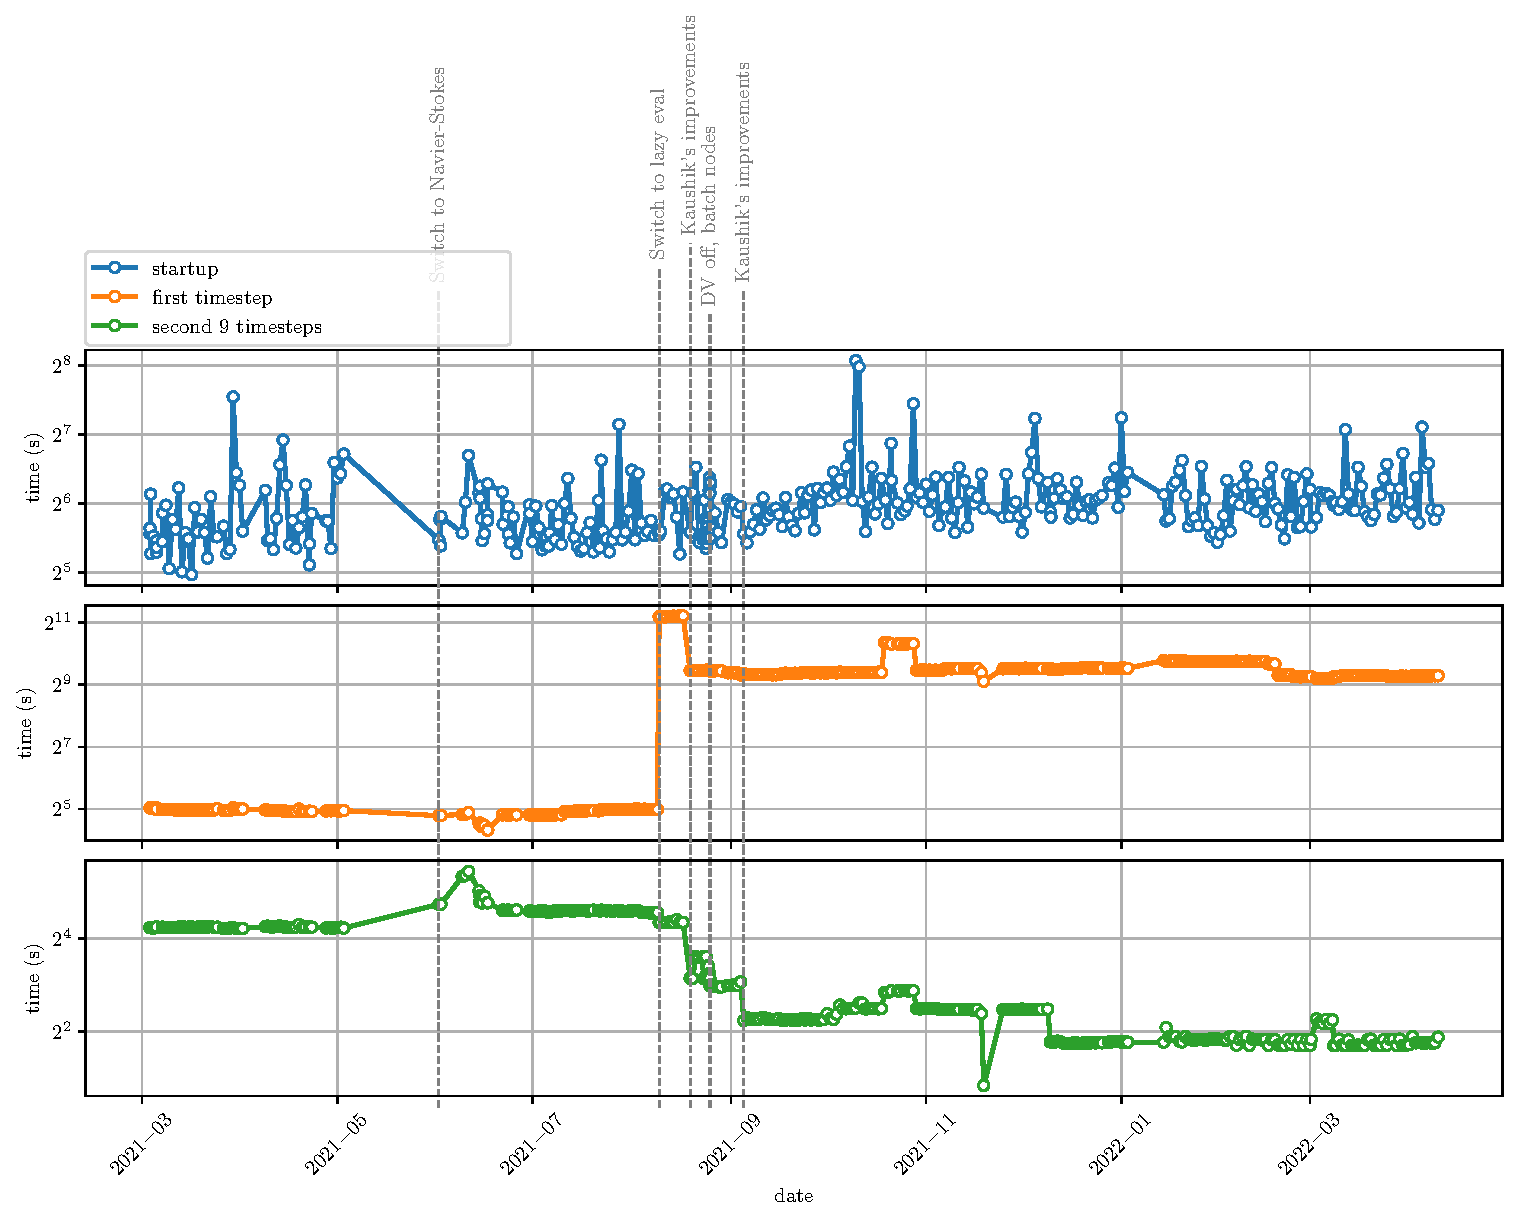
\includegraphics[width=.6\textwidth]{Figures/mtc/nozzle-lazy-full.pdf}
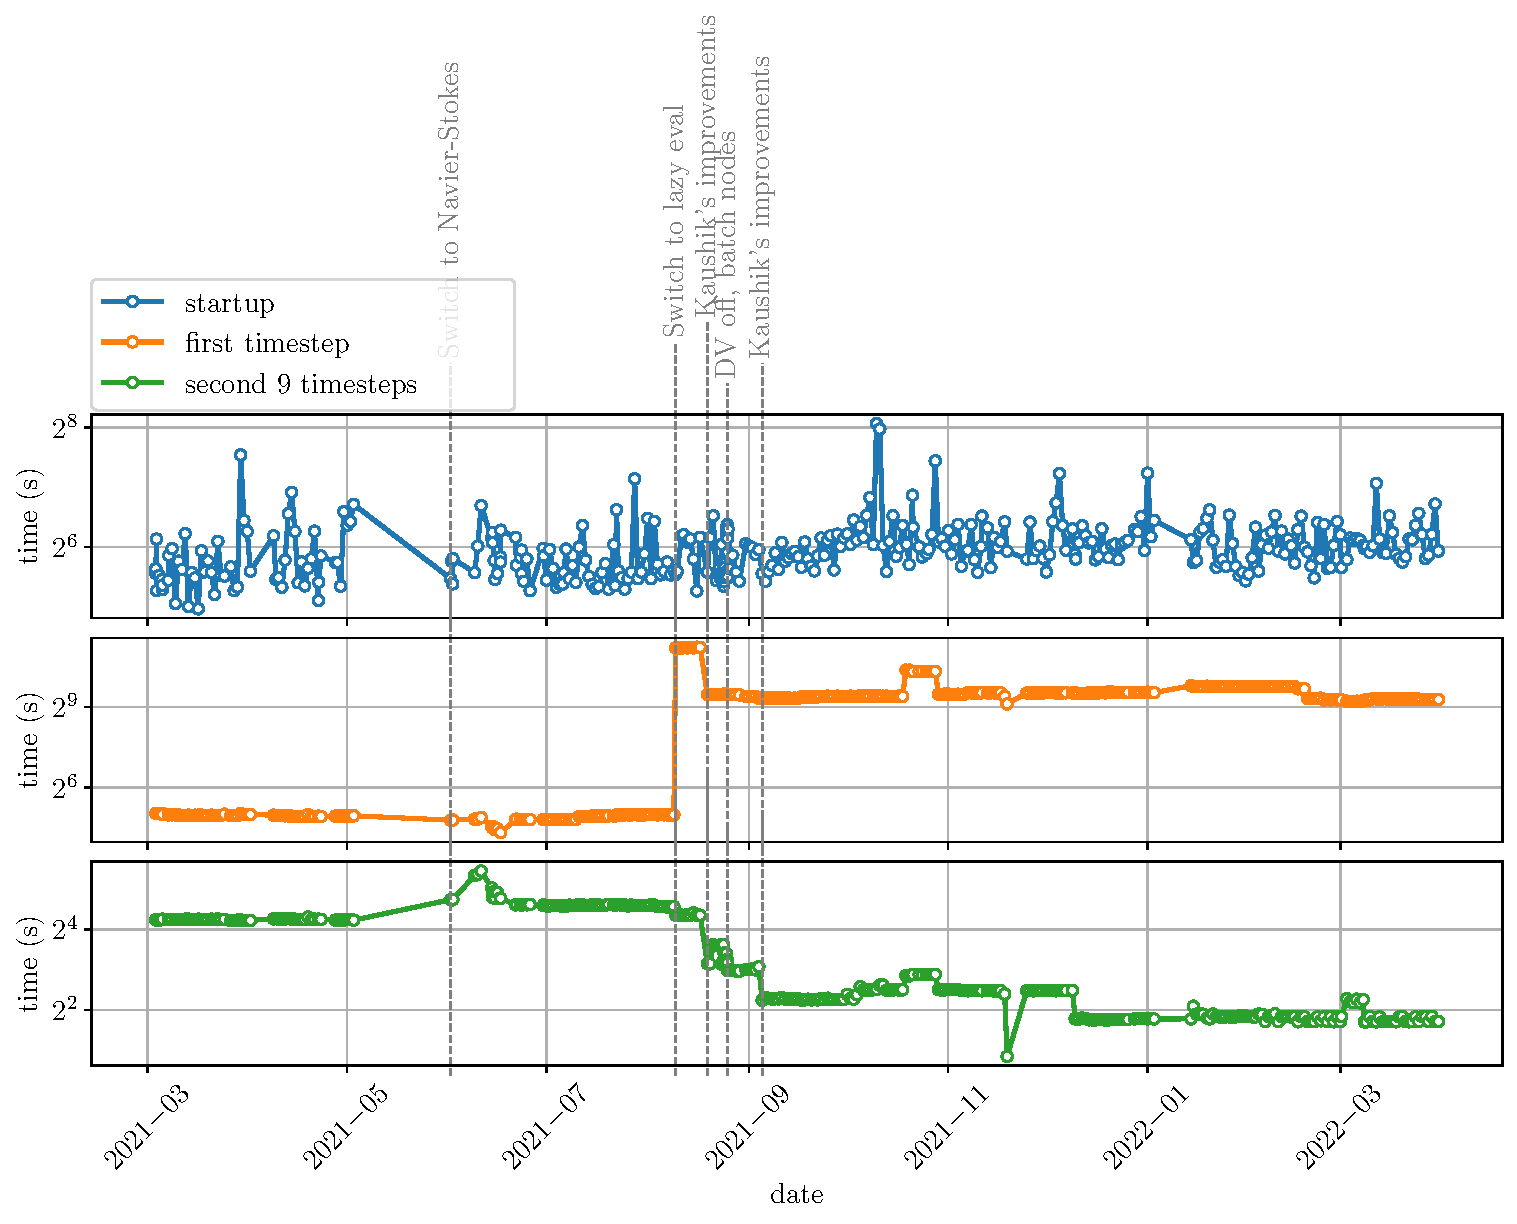
\includegraphics[width=.6\textwidth]{Figures/mtc/big_nozzle_timing_history.pdf}
\end{center}
\end{frame}


\begin{frame}\frametitle{Recent: Persistent Caching of Compiled Kernels}
\begin{center}
  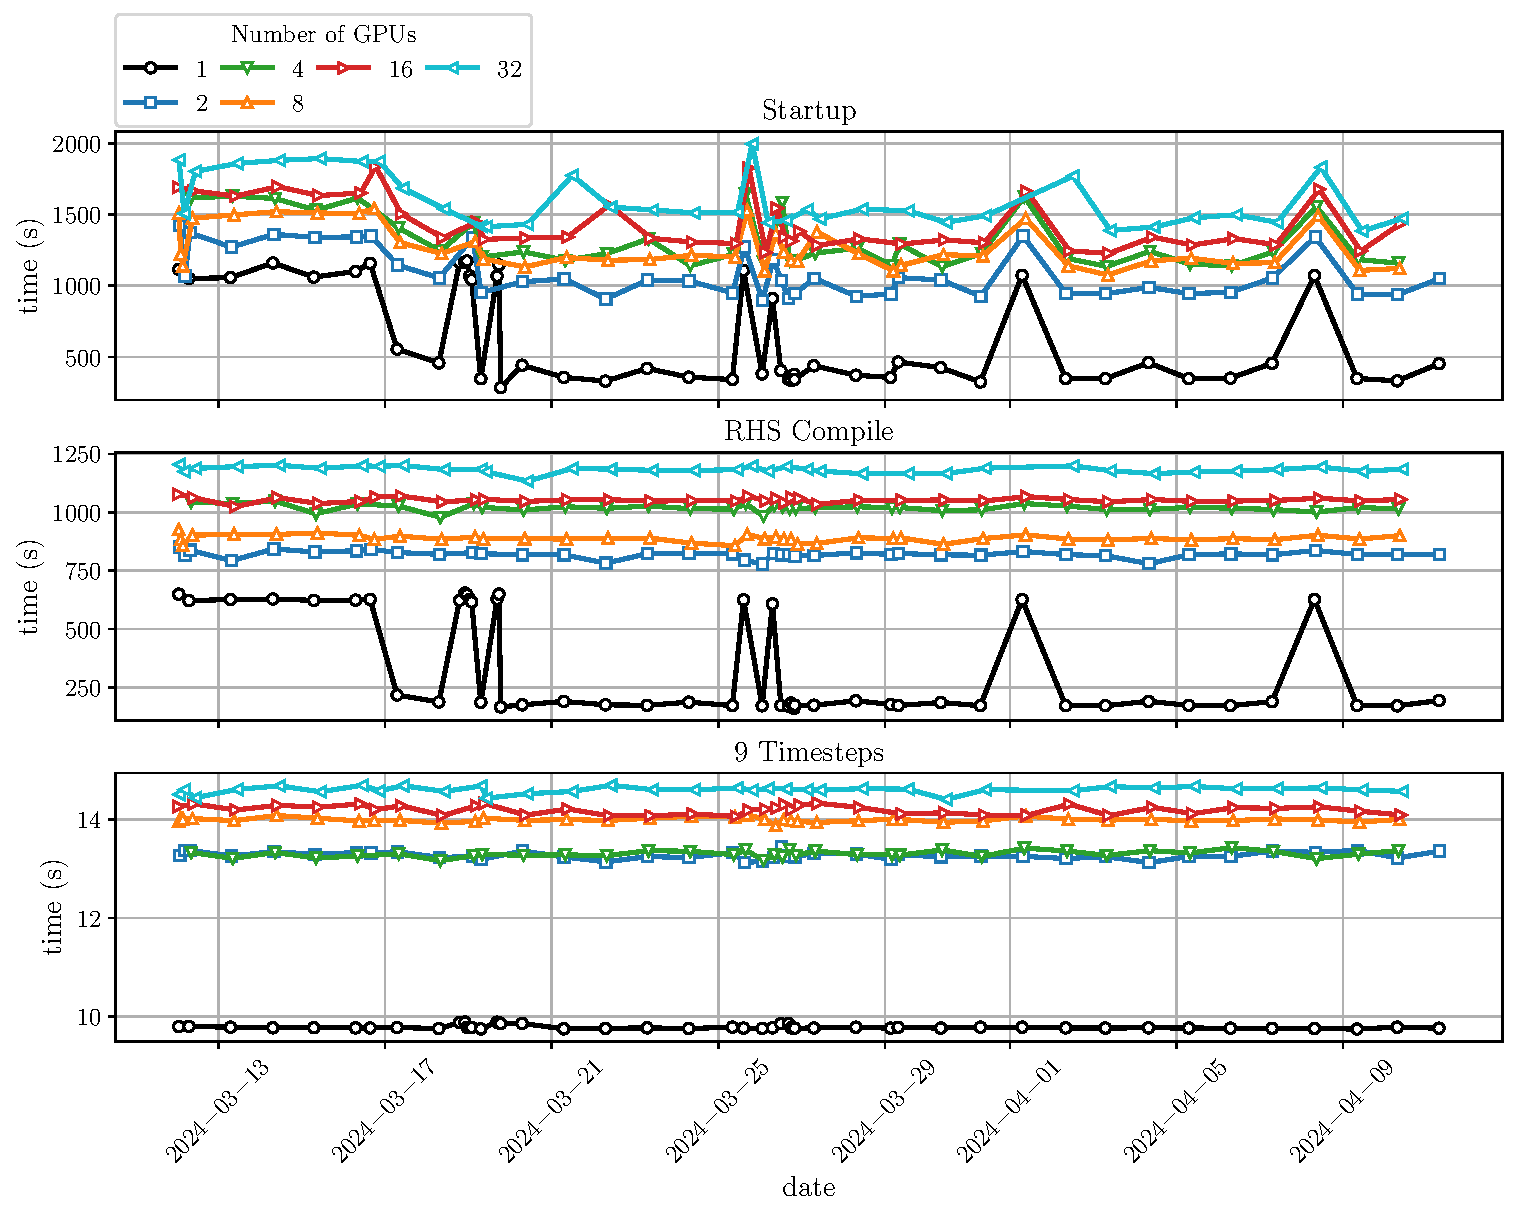
\includegraphics[width=.7\textwidth]{Figures/mtc/y3-recent-cached_1.pdf}
\end{center}
\end{frame}



%\begin{frame}\frametitle{Lifetime Performance Monitoring}
%\centering
%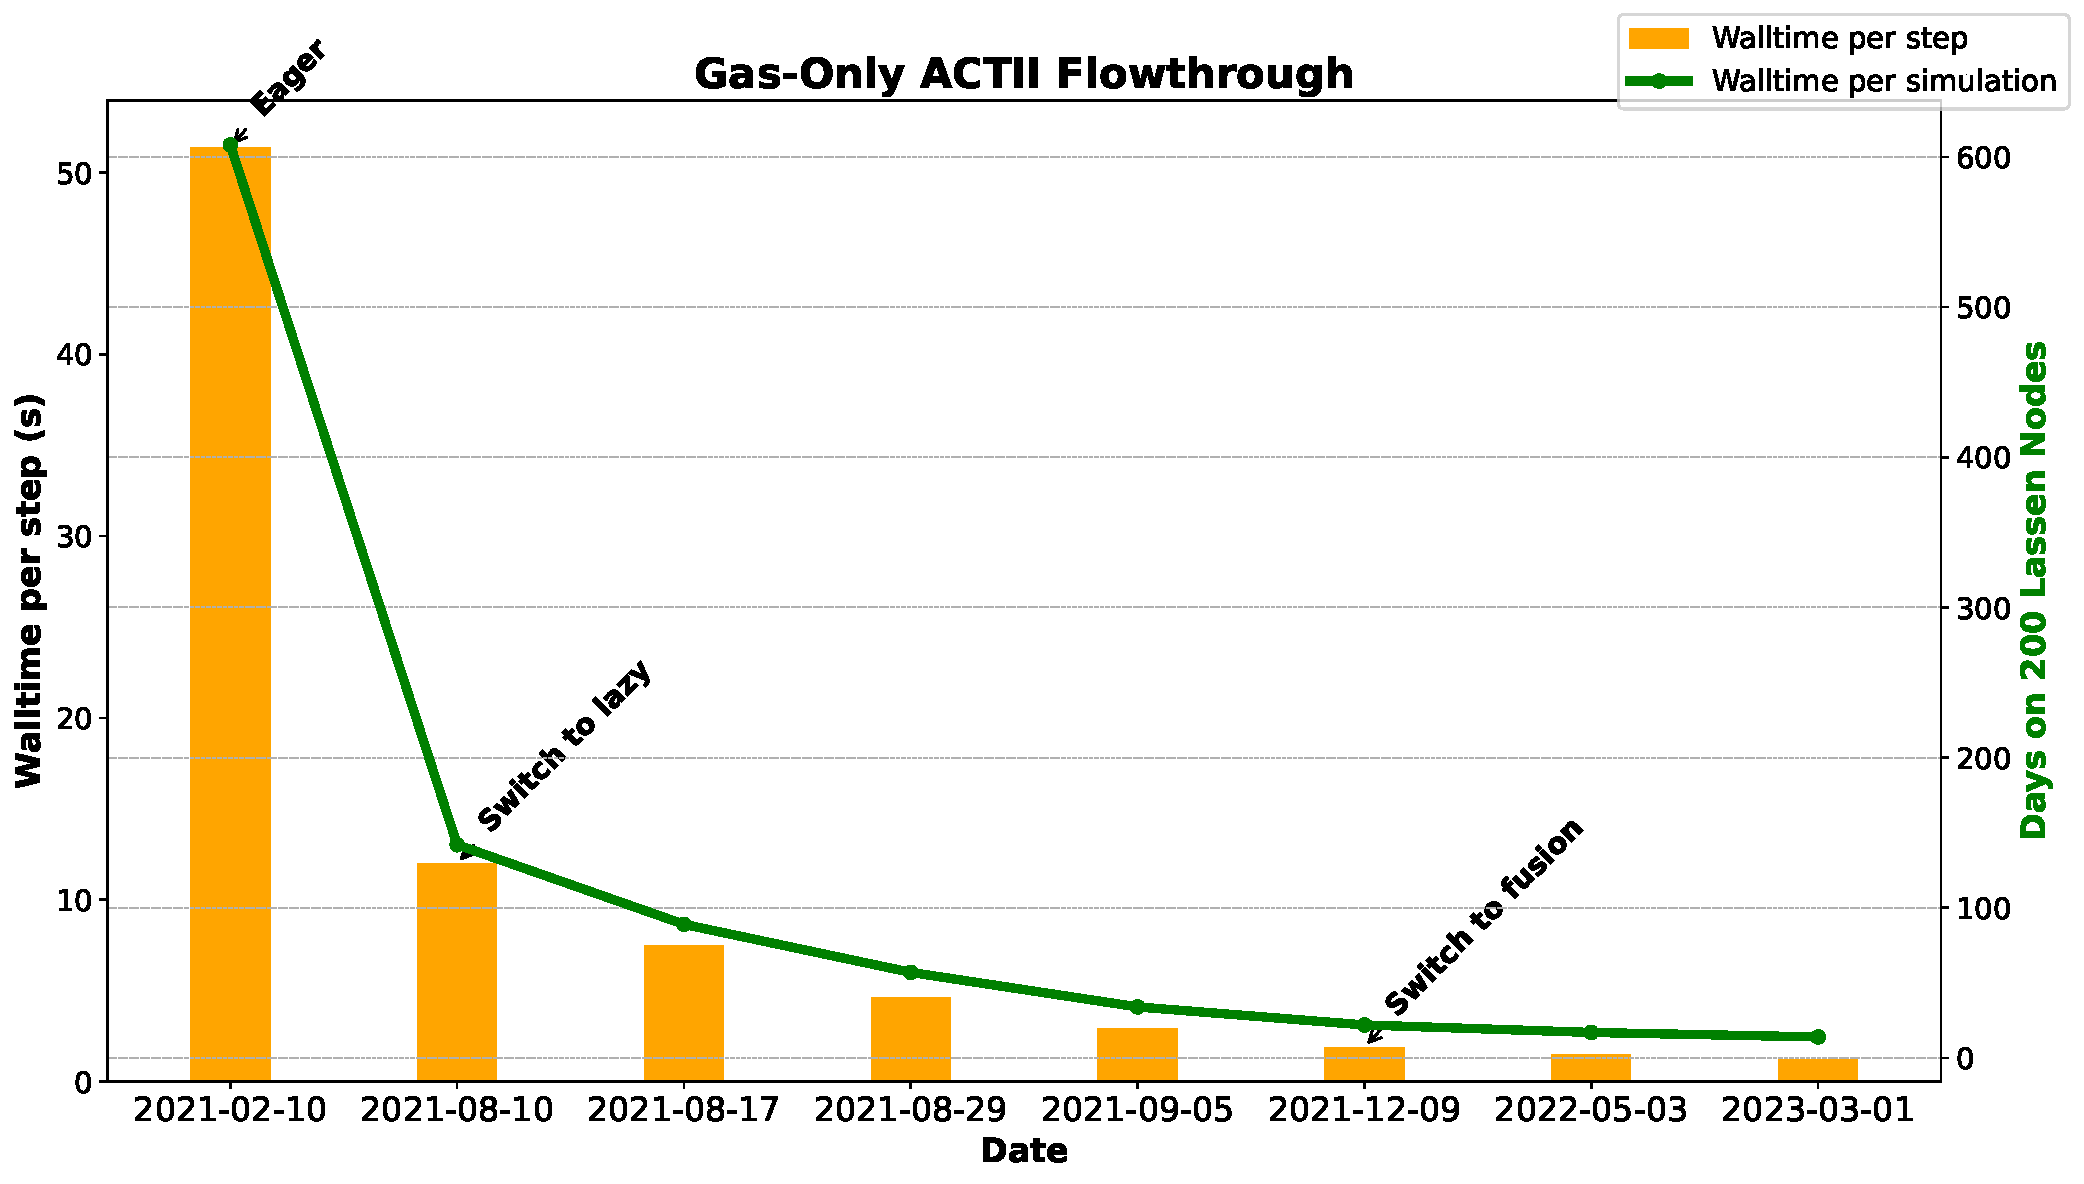
\includegraphics[width=.8\textwidth]{Figures/mtc/gas-only-perf-eager.pdf}
%\end{frame}

\begin{frame}\frametitle{Lifetime Performance Monitoring}
\centering
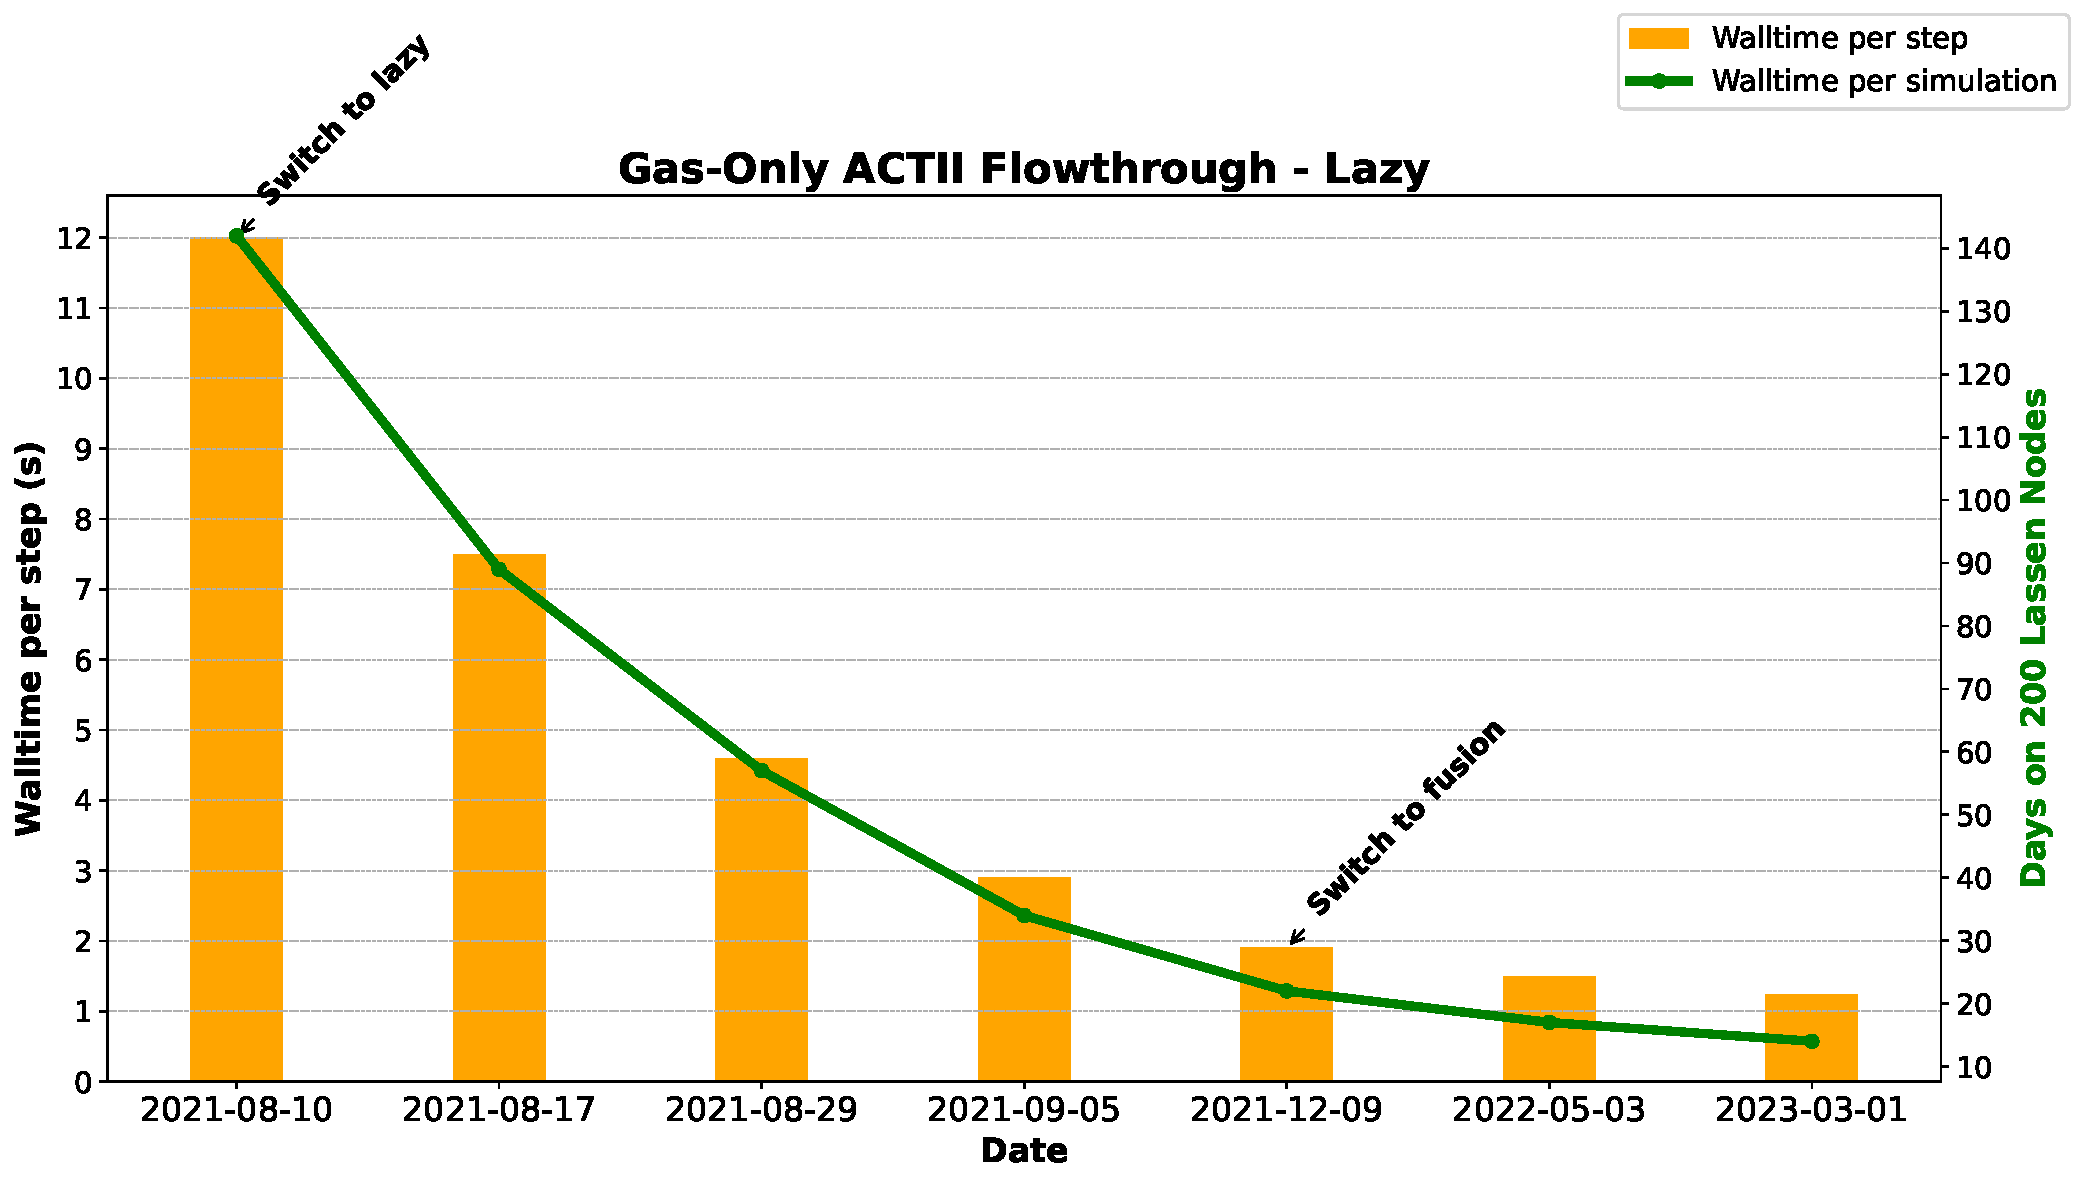
\includegraphics[width=.8\textwidth]{Figures/mtc/gas-only-perf.pdf}
\end{frame}

\begin{frame}\frametitle{Recent Weak Scaling from Nightly KS3D on Lassen}
\begin{center}
  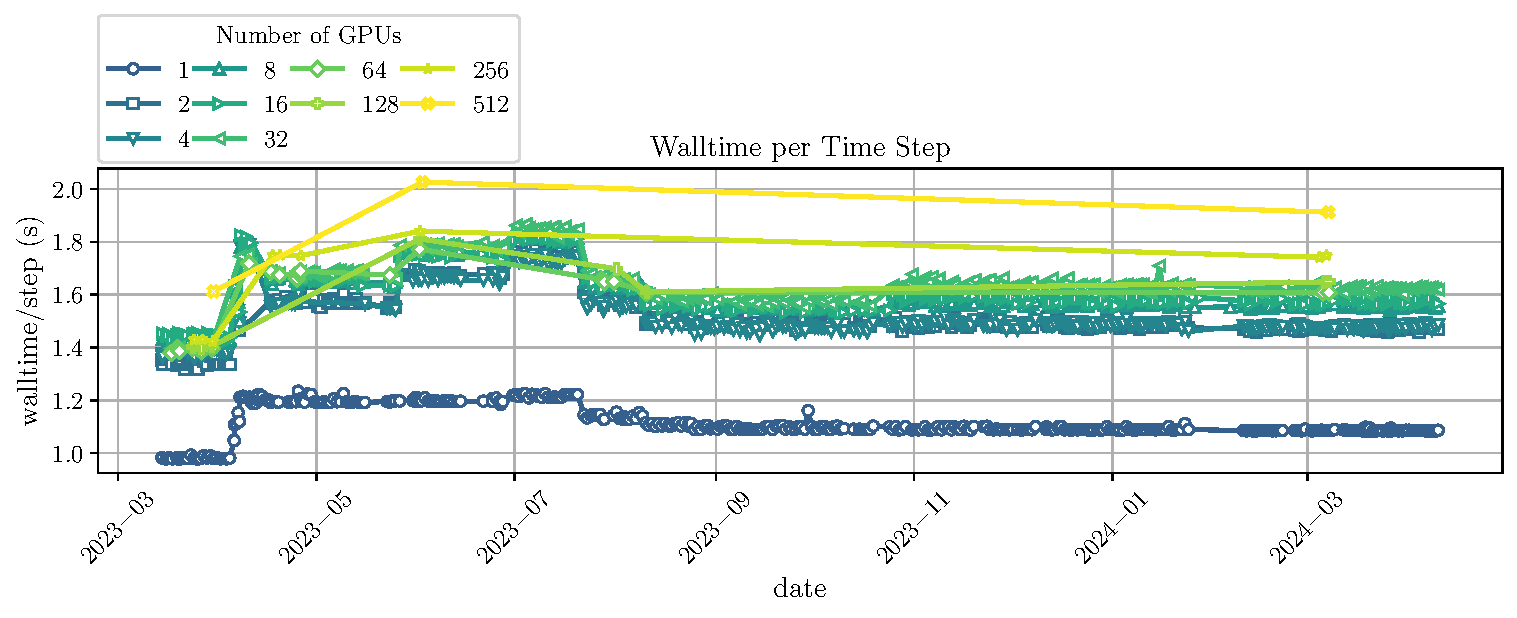
\includegraphics[width=.6\textwidth]{Figures/mtc/NightlyWeak.pdf}
  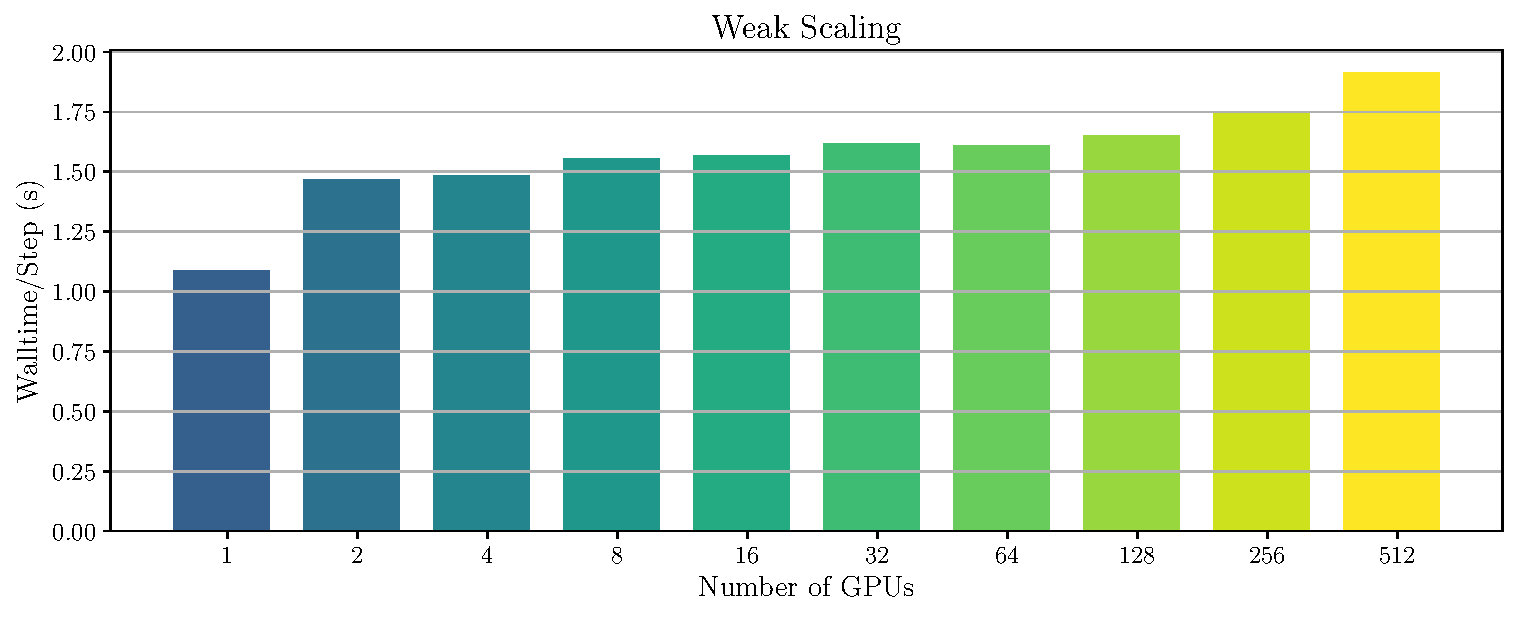
\includegraphics[width=.6\textwidth]{Figures/mtc/weak_scaling_NightlyWeak.pdf}
%\begin{itemize}
%\item KS3D: Prediction physics, 24k $p=4$ Tets / MPI rank
%\end{itemize}
\end{center}
\end{frame}

\begin{frame}\frametitle{Lassen DATs for Testing at Scale}
  \begin{itemize}
  \item Current performance supports prediction-scale simulation
  \item Dedicated Application Time (DAT) for prediction last Fall 
  \item Large portion of Lassen:
    \begin{itemize}
    \item 512 / 600(ish) available nodes
    \item 4$\times$NVIDIA Volta (V100) GPUs / node
    \item 256GB of host RAM, 16GB per GPU, Unified mem
    \end{itemize}
  \end{itemize}
\end{frame}

\begin{frame}\frametitle{Scalability Data from Lassen DAT}
    \begin{columns}[T]  % [T] is for top vertical alignment

    % Left Column
    \begin{column}{0.5\textwidth}
    \centering
    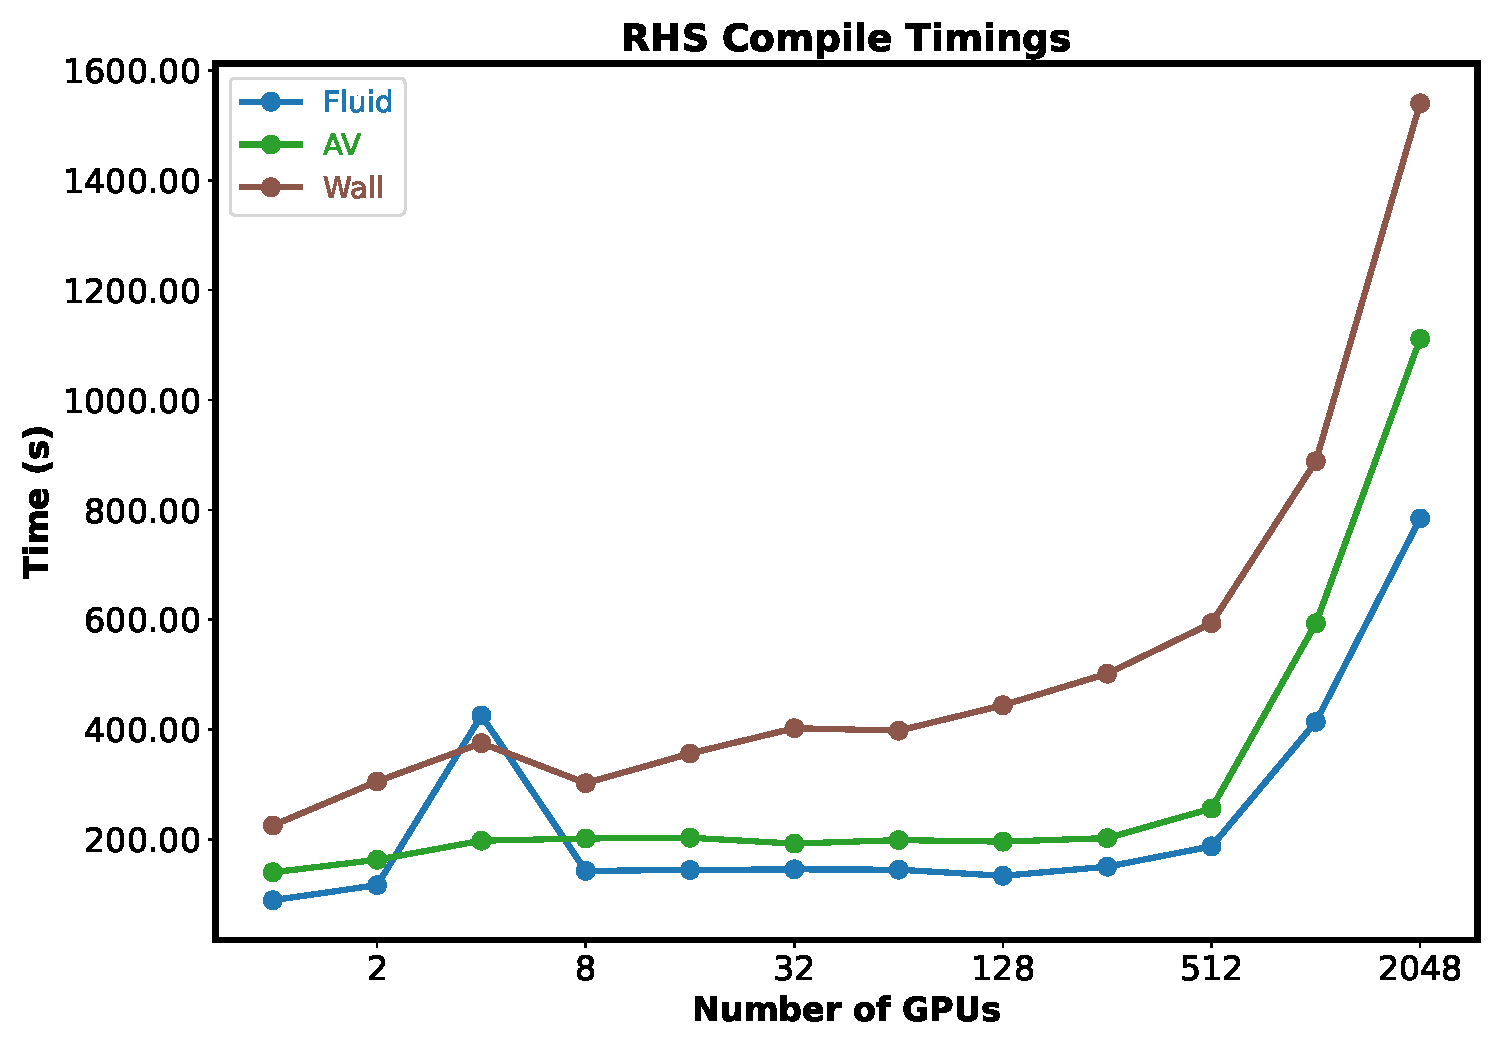
\includegraphics[width=\textwidth]{Figures/mtc/RHSCompileTimes_2048.pdf}
    \end{column}
    
    % Right Column
    \begin{column}{0.5\textwidth}
    \centering
      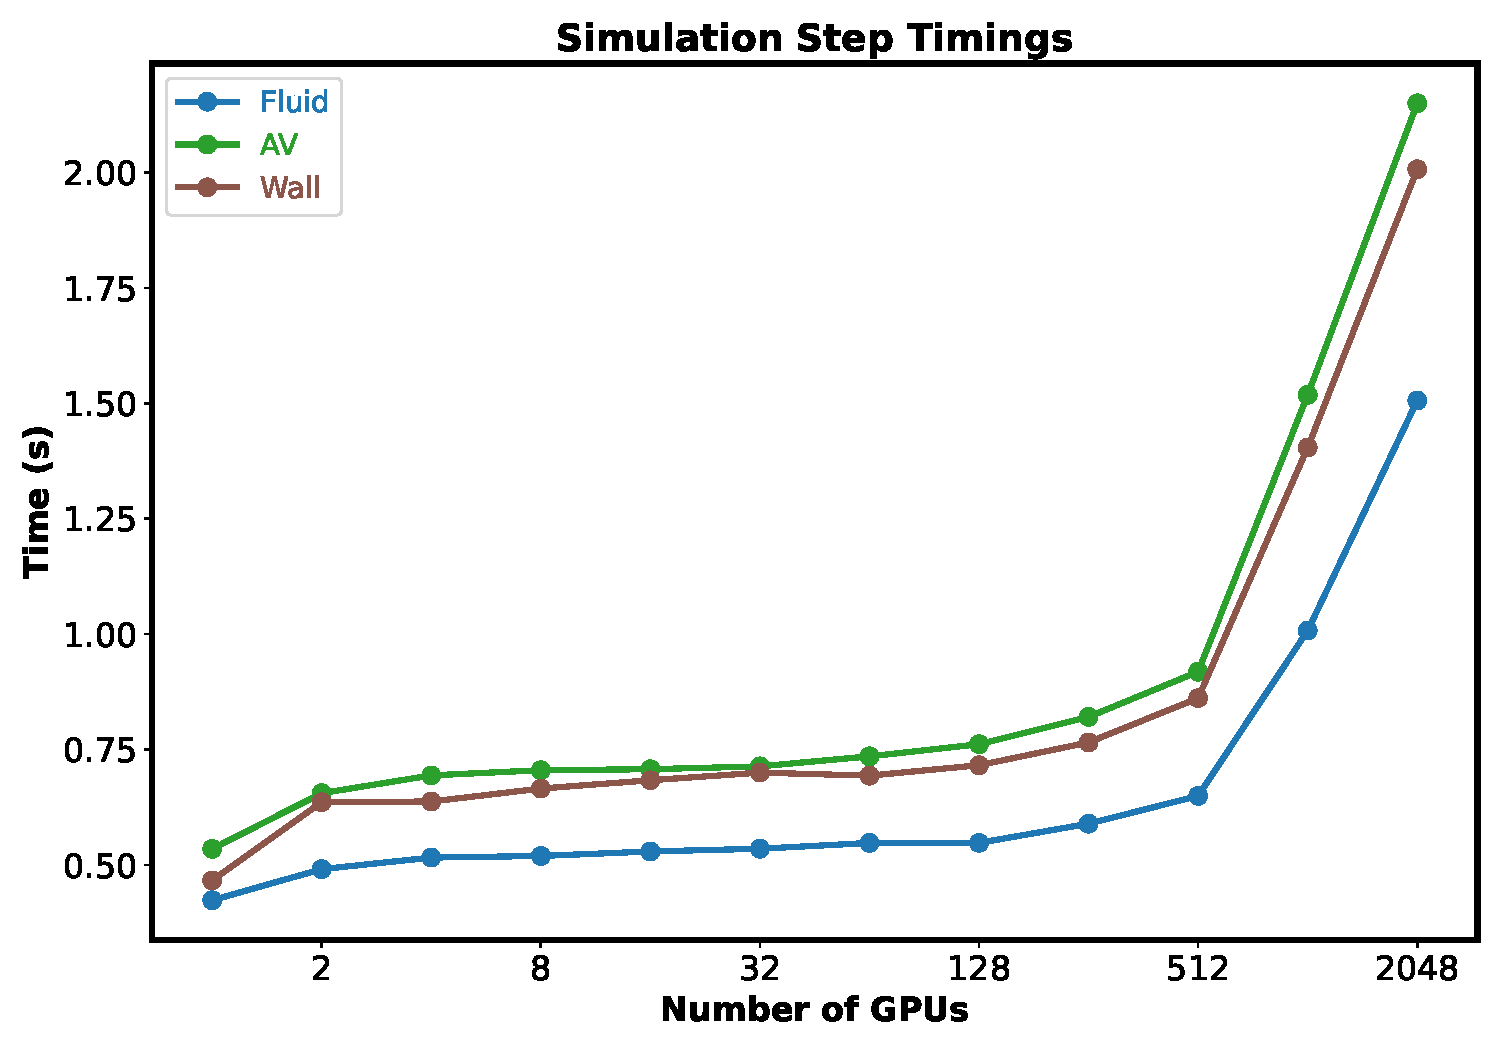
\includegraphics[width=\textwidth]{Figures/mtc/SimulationStepTimes_2048.pdf}
    \end{column}

  \end{columns}
  \begin{center}
  \begin{itemize}
  \item Prediction geometry, weak scaling with 24k $p=4$ Tets per MPI rank
  \item Compile and per-step timings for Fluid-only, Artificial Viscosity (AV), and Fluid-Wall-AV 
  \end{itemize}
  \end{center}
\end{frame}

\begin{frame}
    \centering
    \Large
    Challenges To Performance
\end{frame}

\begin{frame}\frametitle{Recall: DAG Splat Effect}
\vspace{5pt}
  \begin{minipage}{0.49\textwidth}		
    \begin{itemize}
    \item Unexpected DAG scaling vs. MPI ranks
    \item DAG \textit{splat}: function DAG inlining:
    \begin{itemize}
    \item Flux: BCs \& Interior boundaries (IEB)
    \item Temperature: Newton iterations
    %\item Function \texttt{make\_fluid\_state} (MFS)
    %\item Dependent vars (DV): Newton iters
    %\item BCs \& Interior boundaries (IEB)
    \end{itemize}
    \item 1D part: Particle board $\rightarrow$ pancakes
    \end{itemize}
    \begin{center}
    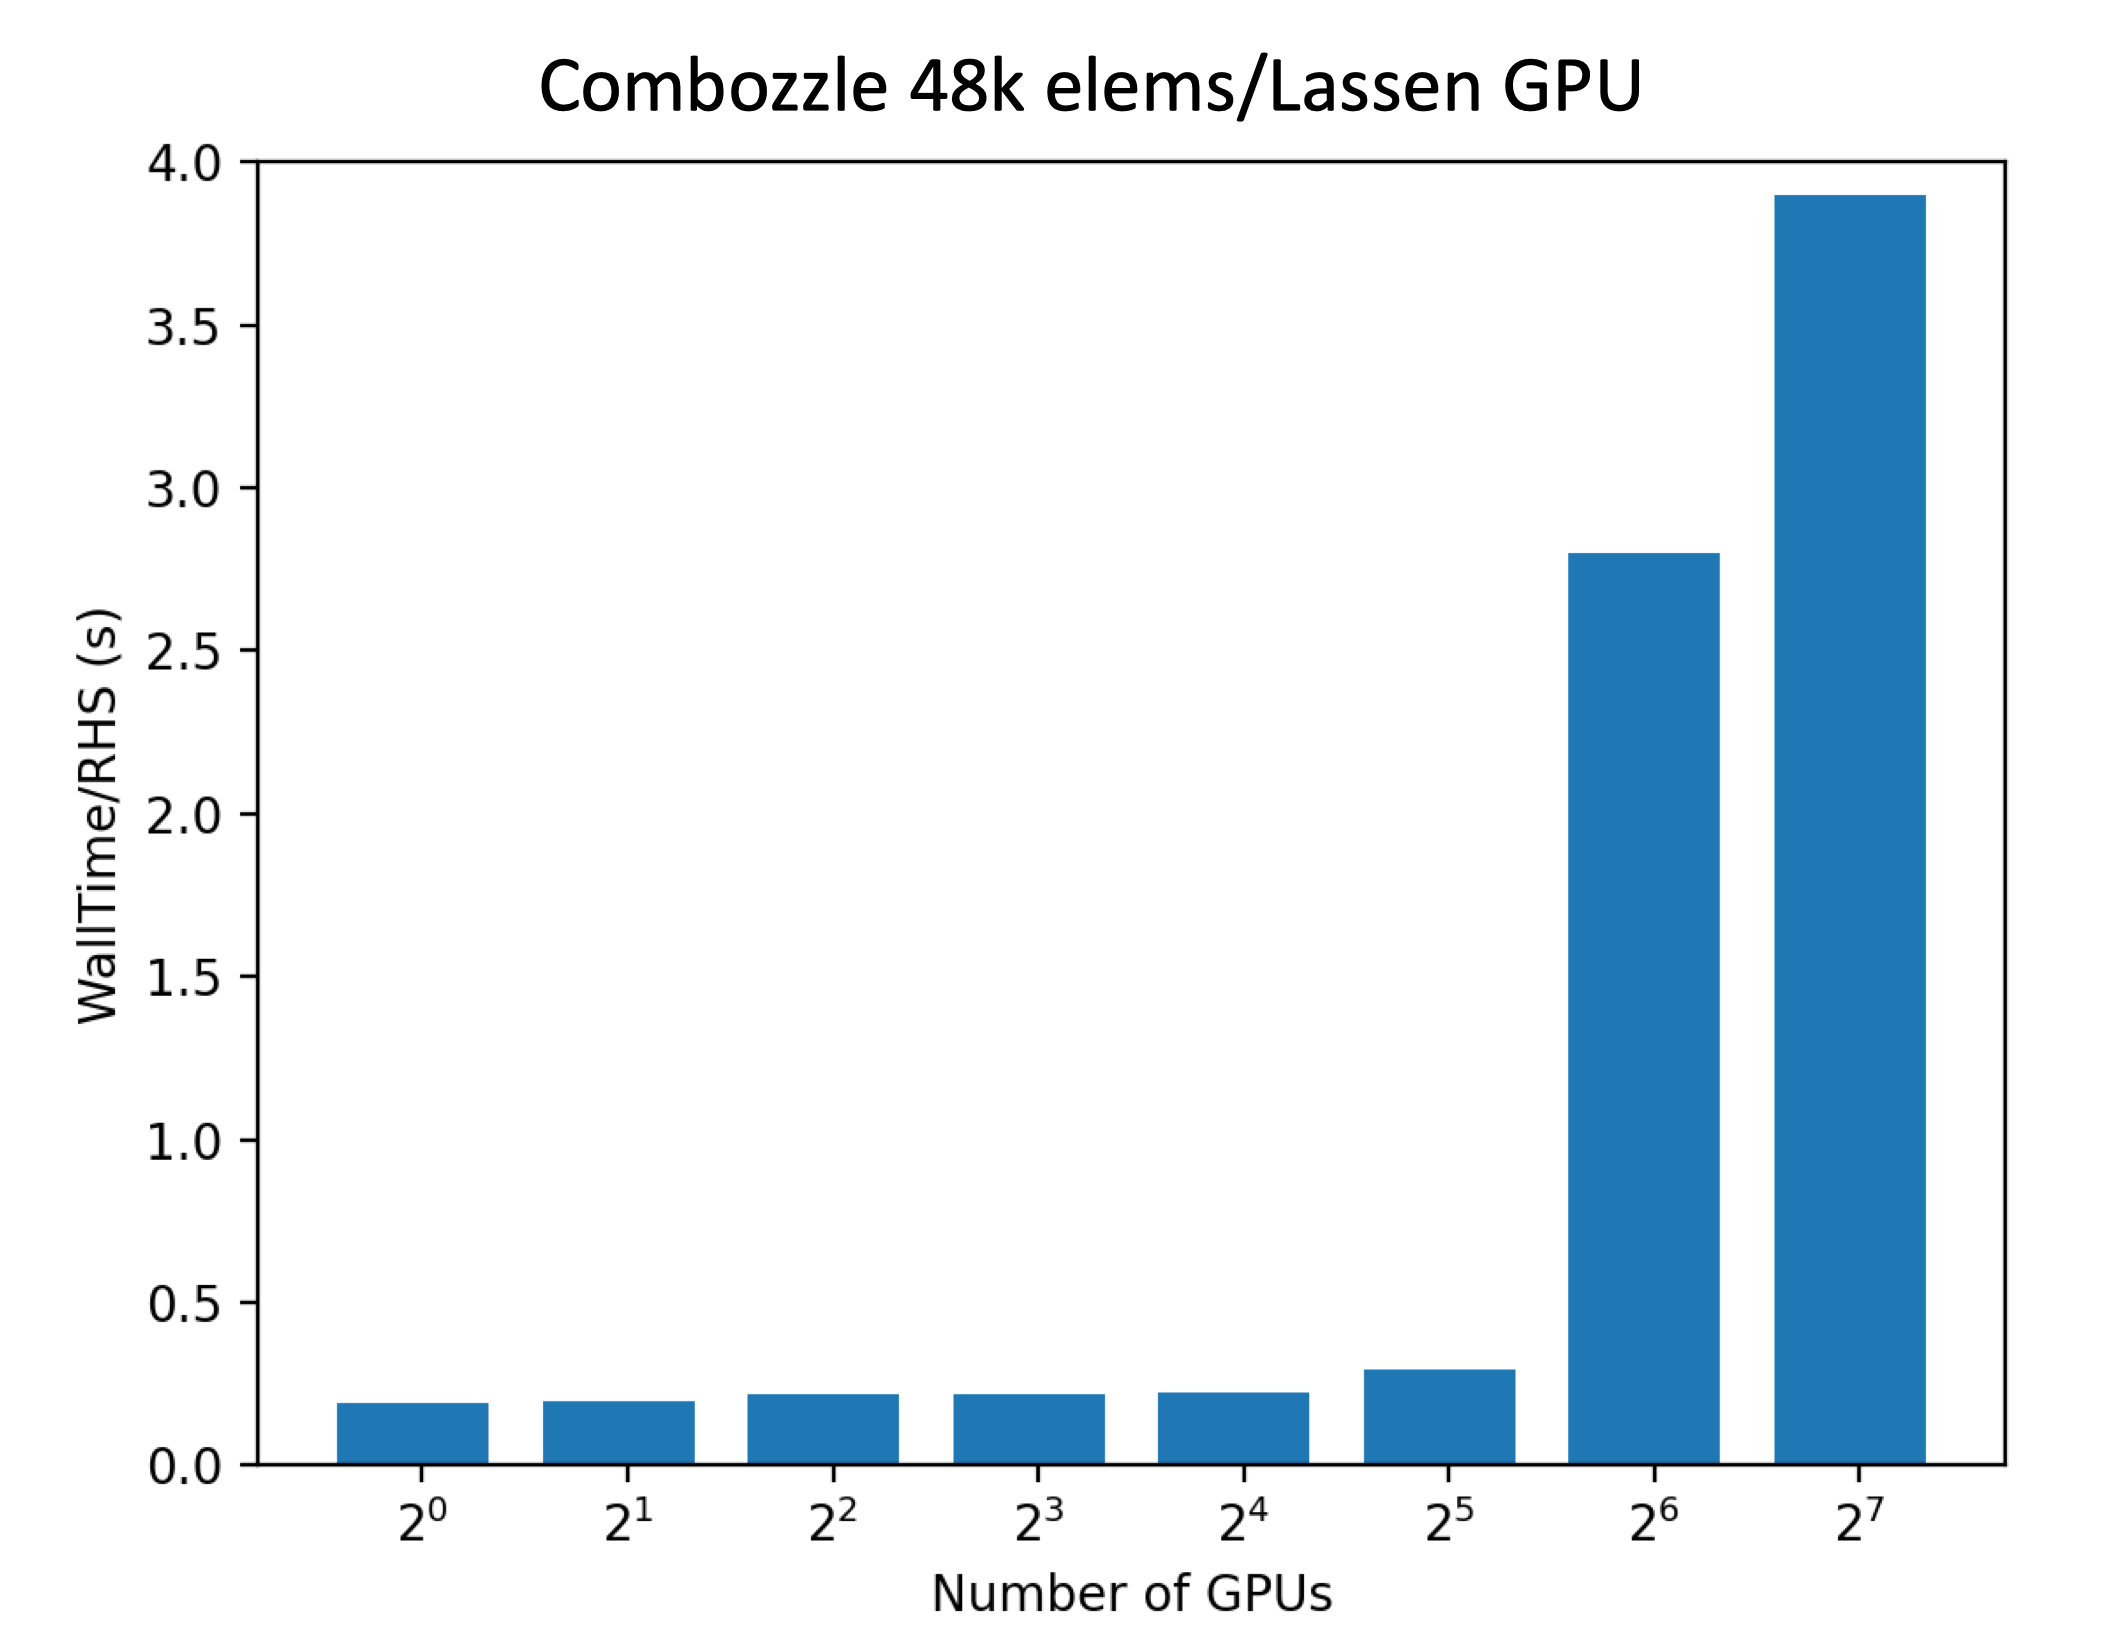
\includegraphics[width=.8\textwidth]{Figures/mtc/combozzle_weak_bad_partitioning.png}
    \end{center}
  \end{minipage}
  \begin{minipage}{0.49\textwidth}
    %\begin{figure}
      \centering
      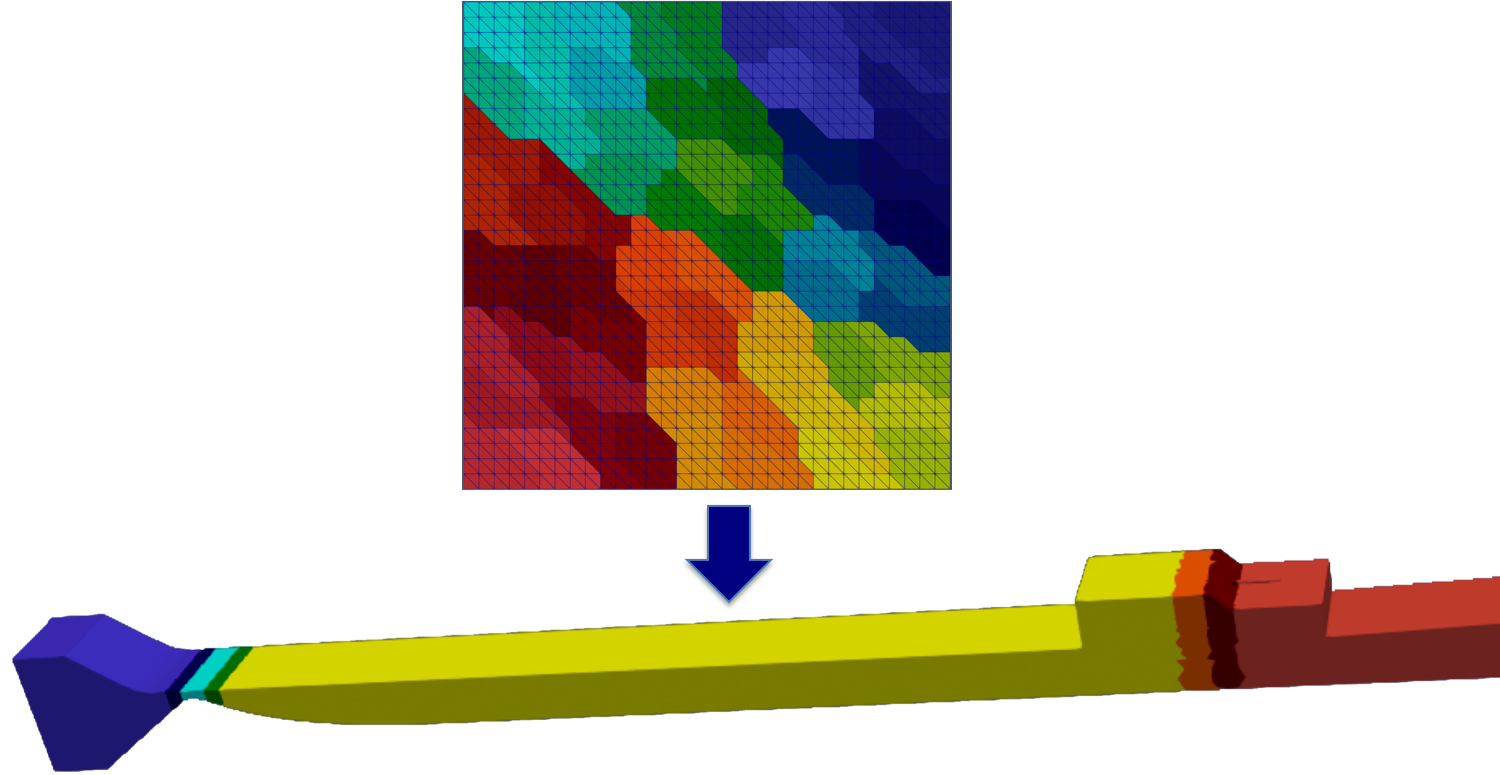
\includegraphics[width=.8\textwidth]{Figures/mtc/MetisTo1D.png} \\
      \vspace{10pt}
    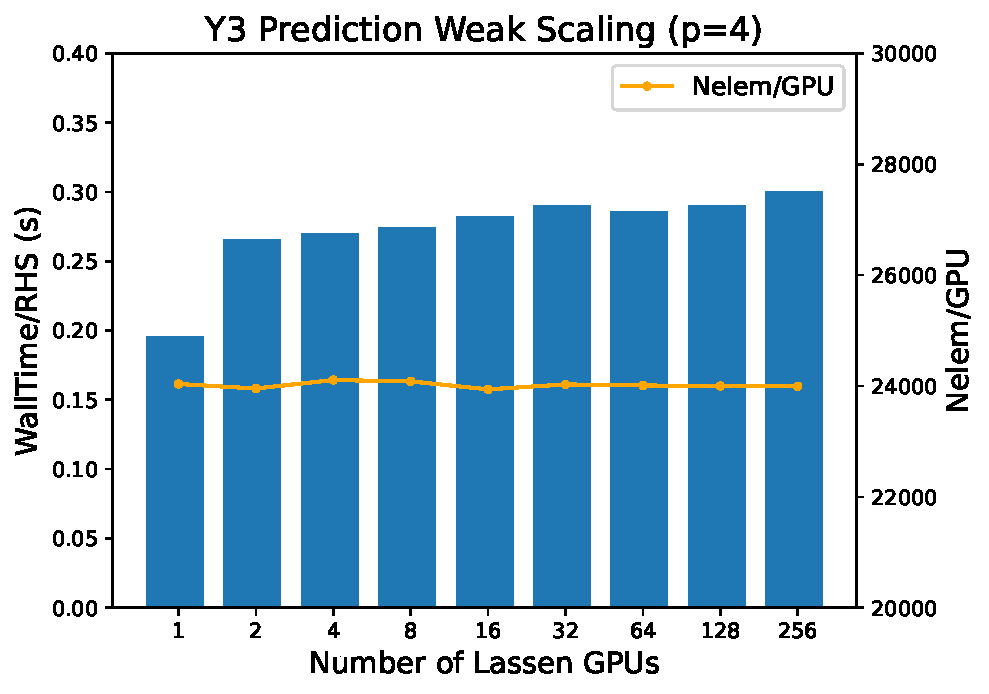
\includegraphics[width=.8\textwidth]{Figures/mtc/y3-prediction_weak_scaling.pdf}
    %\end{figure}		
  \end{minipage}
\end{frame}


\begin{frame}\frametitle{DAG Splat Rises Again: No Surprises}
    \begin{columns}[T]  % [T] is for top vertical alignment
    % Left Column
    \begin{column}{0.5\textwidth}
      % Top left: Text
      \begin{itemize}
      \item DAG Splat is the culprit for full machine scaling fail
      \item 1D Partitioning fails spectacularly at scale
      \item Pancakes $\rightarrow$ waffles
      \item Material-material interfaces contribute significantly to DAG
      \end{itemize}
      \vspace{20pt}
      \hspace{20pt}
      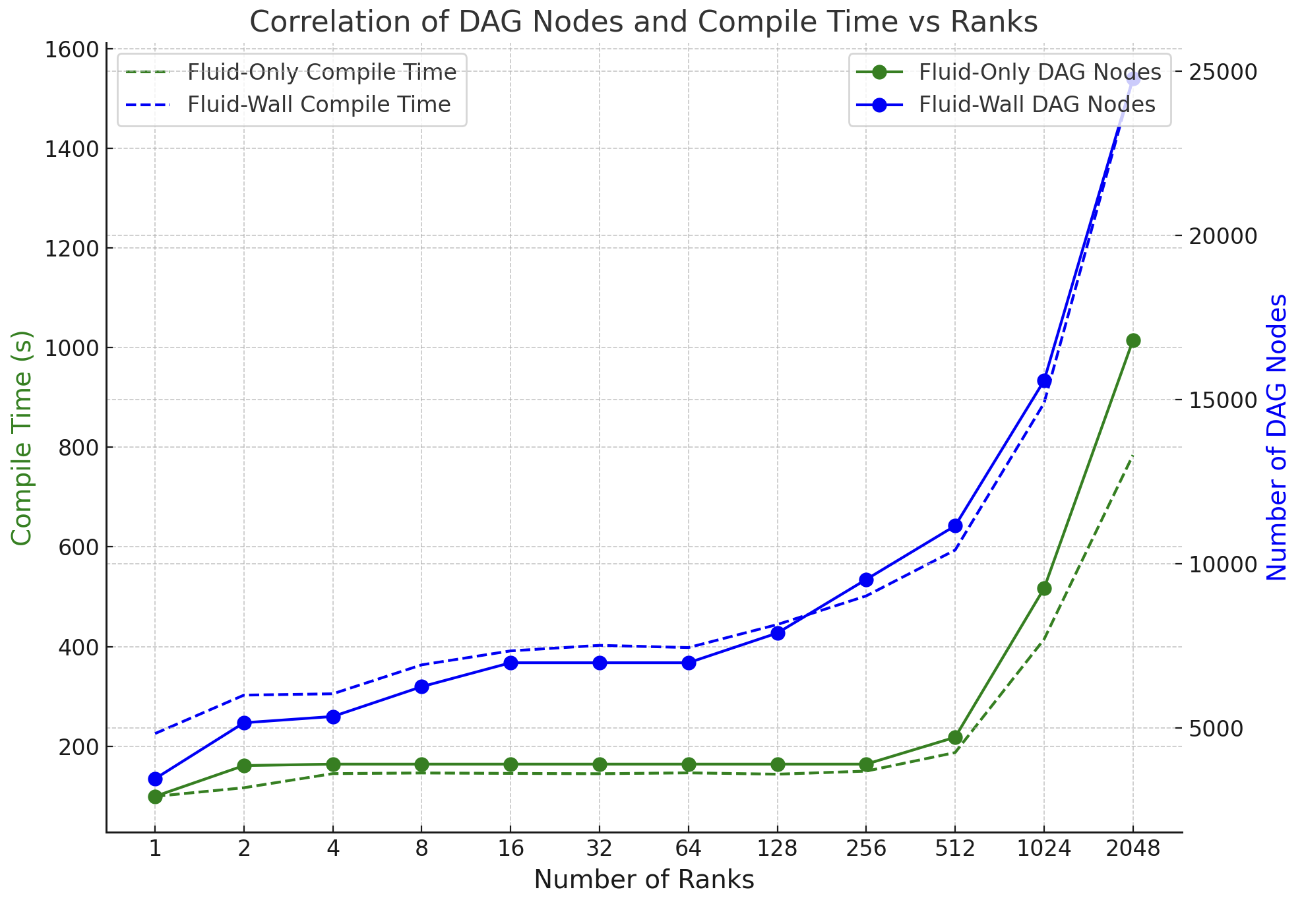
\includegraphics[width=.7\textwidth]{Figures/mtc/compile_times_dag_nodes.png}
    \end{column}
    
    % Right Column
    \begin{column}{0.5\textwidth}
      \vspace{-15pt}
      \hspace{20pt}
      % Top right: Startup Times
      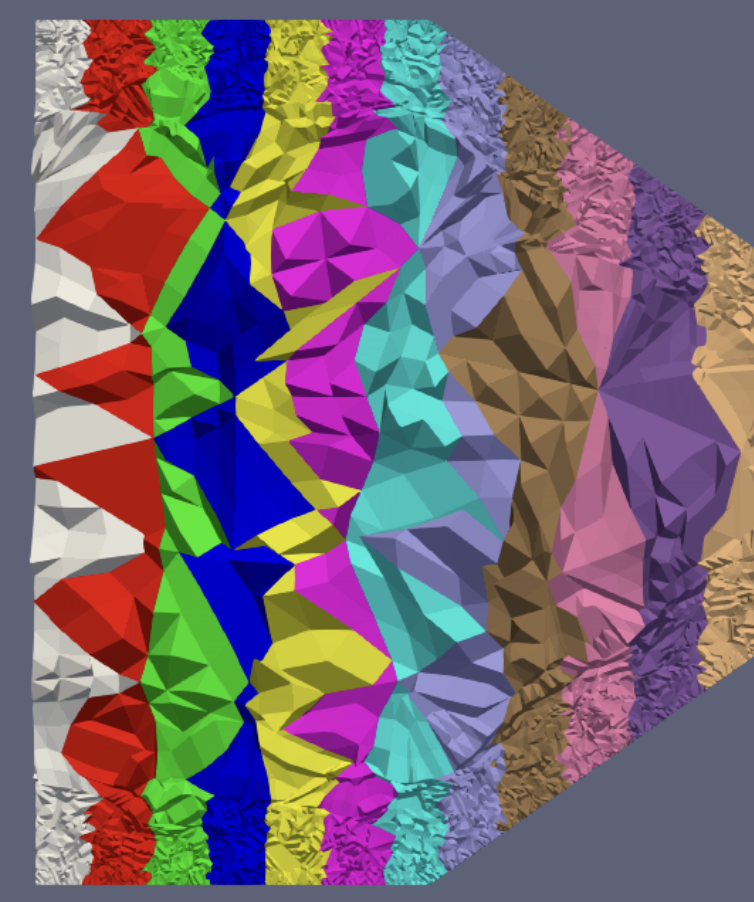
\includegraphics[width=.4\textwidth]{Figures/mtc/BadPartitioning2.png}
      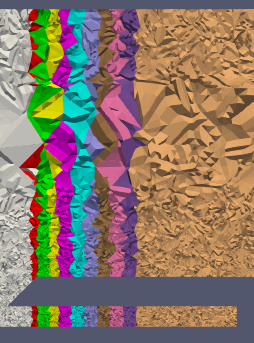
\includegraphics[width=.4\textwidth]{Figures/mtc/BadPartitioning.png}
      % Bottom right: Simulation Step Times
      \vfill
      \vspace{10pt}
      \hspace{20pt}
      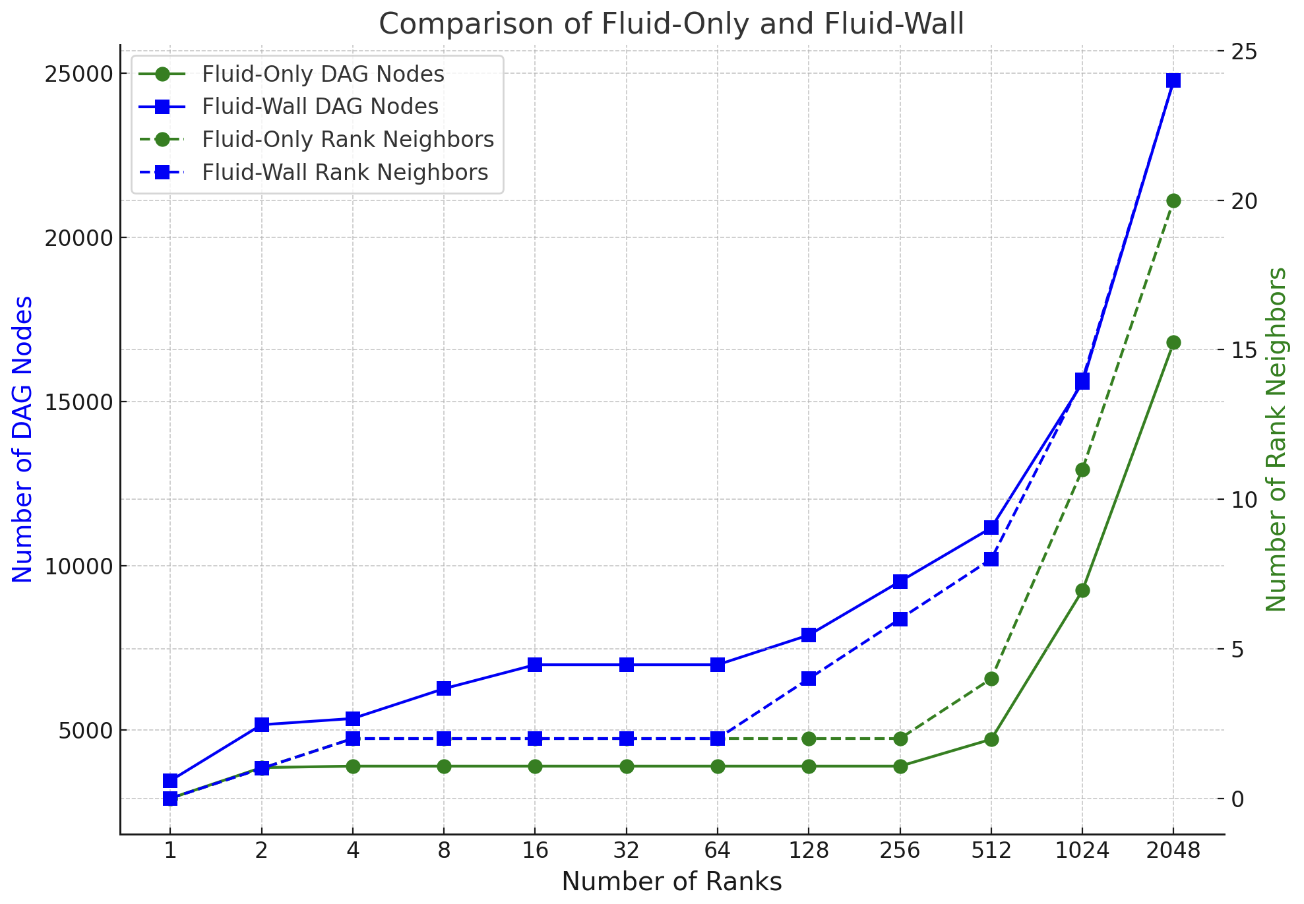
\includegraphics[width=.7\textwidth]{Figures/mtc/dag_nodes_rank_nbrs.png}
    \end{column}
  \end{columns}
\end{frame}

\begin{frame}\frametitle{What Makes Prediction DAGs So Big?}
\begin{columns}[T, onlytextwidth] % Aligns contents at the top
    \begin{column}{0.48\textwidth}
        \begin{itemize}
          \item Which features cause DAG explosion?
          \begin{itemize}
          \item Dependent var (DV) evals are expensive (mixtures)
          \item \texttt{make\_fluid\_state} (MFS): many DV evals (limiting)
          \end{itemize}
          \item Compile times grow faster than the DAG
        \end{itemize}
        \vspace{10pt}
        \centering
        %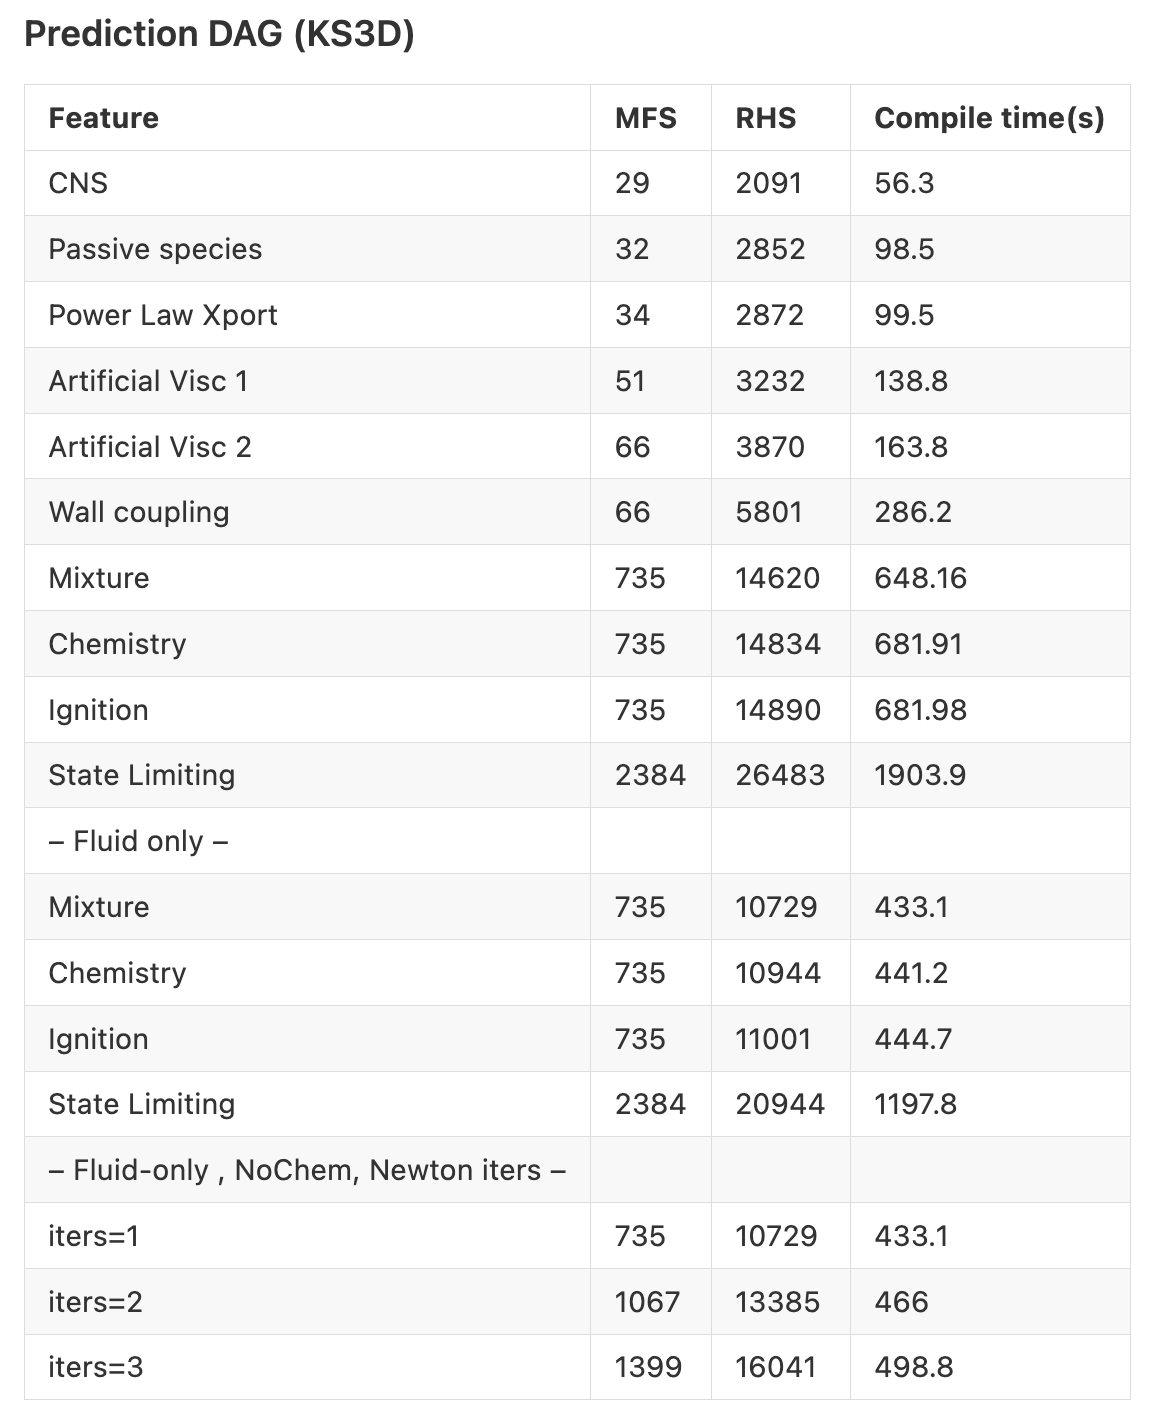
\includegraphics[width=.8\textwidth]{Figures/mtc/prediction_dag_table.png}
        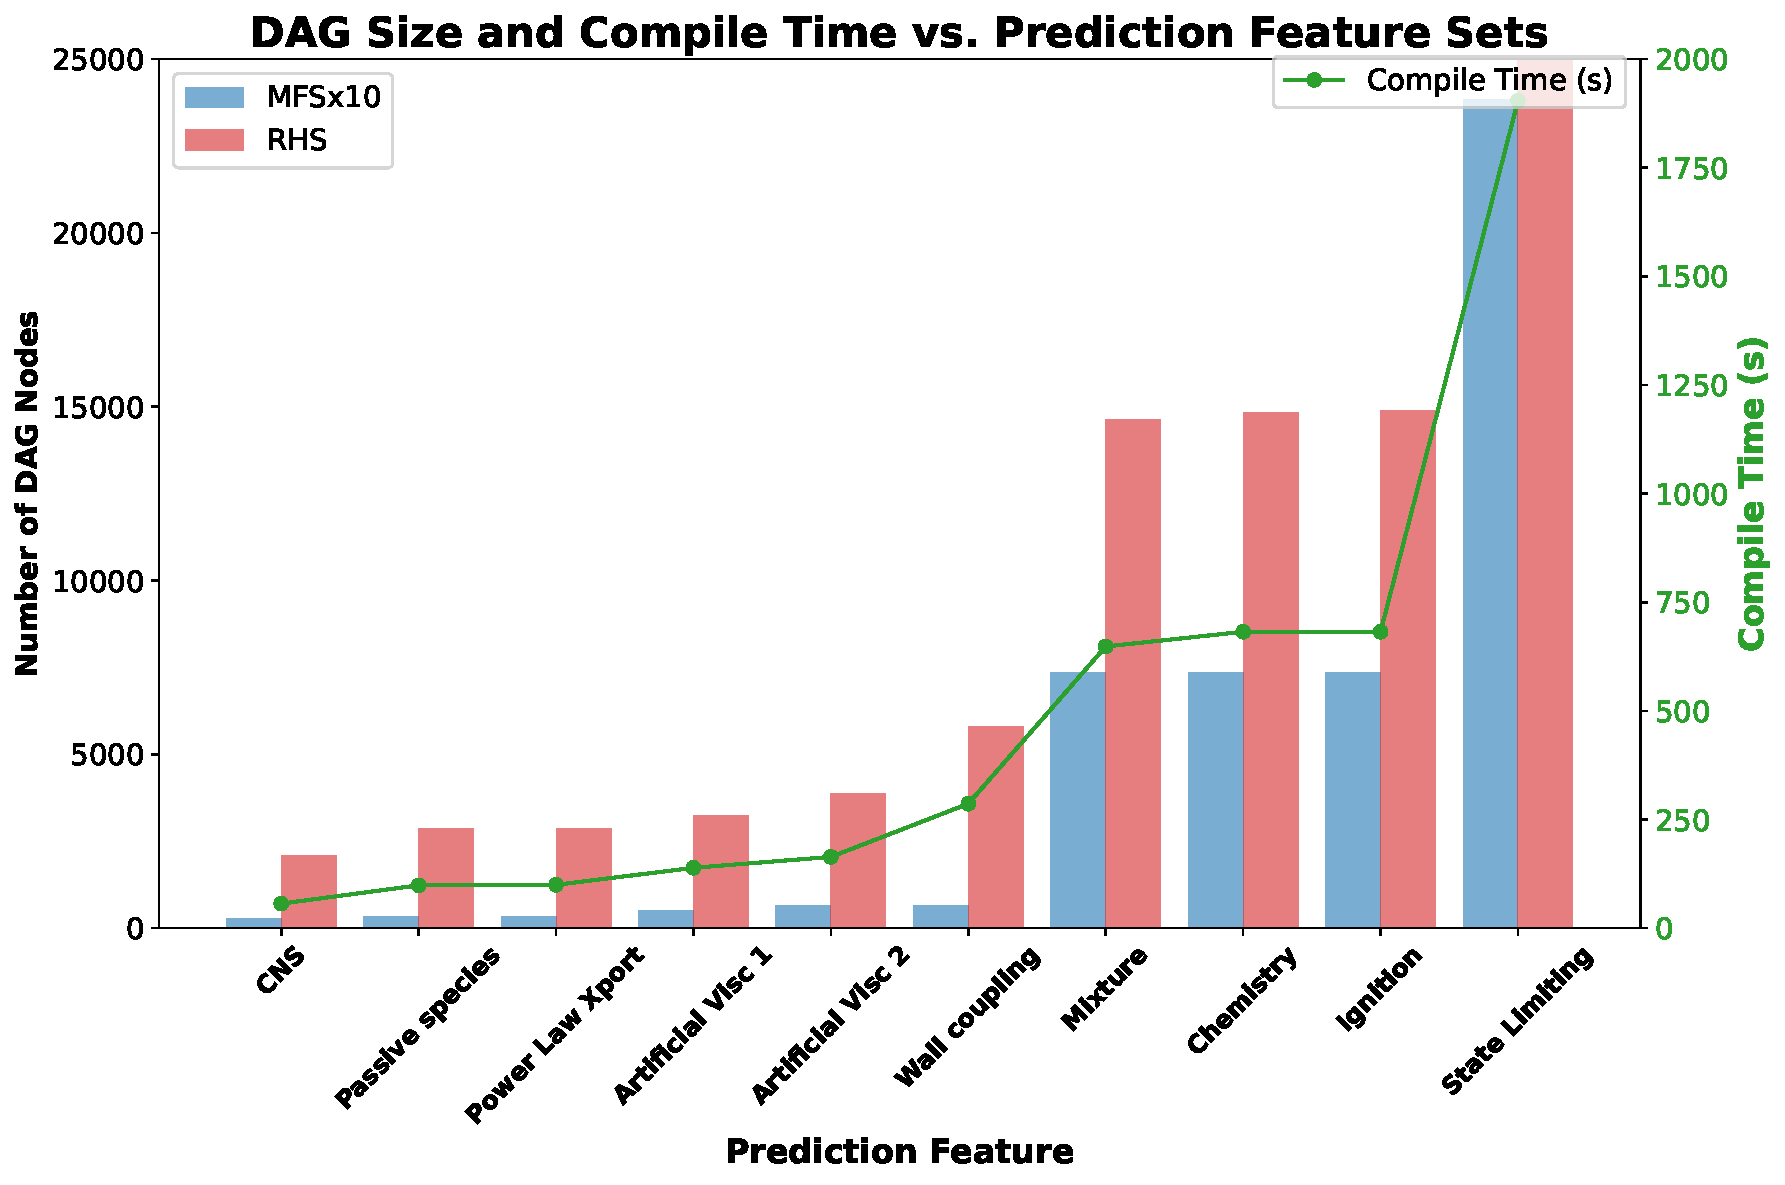
\includegraphics[width=\textwidth]{Figures/mtc/prediction_features_dag.pdf}
    \end{column}

    \begin{column}{0.48\textwidth}
        \centering
        \begin{tabularx}{\textwidth}{|X|X|X|X|X|}
            \hline
            \textbf{Gas} & \textbf{Vol} & \textbf{BC} & \textbf{IEB} & \textbf{Total} \\ \hline
            Single & 290 & 486 & 697 & 1473 \\ \hline
            Mixture & 1591 & 2500 & 3060 & 7151 \\ \hline
        \end{tabularx}        
        \vspace{5pt}
        $N_{\text{dag}} = 1591 + 2500(N_{\text{bc}}) + 3060(1 + N_{\text{pb}})$\\
        \vfill
        \vspace{20pt}
        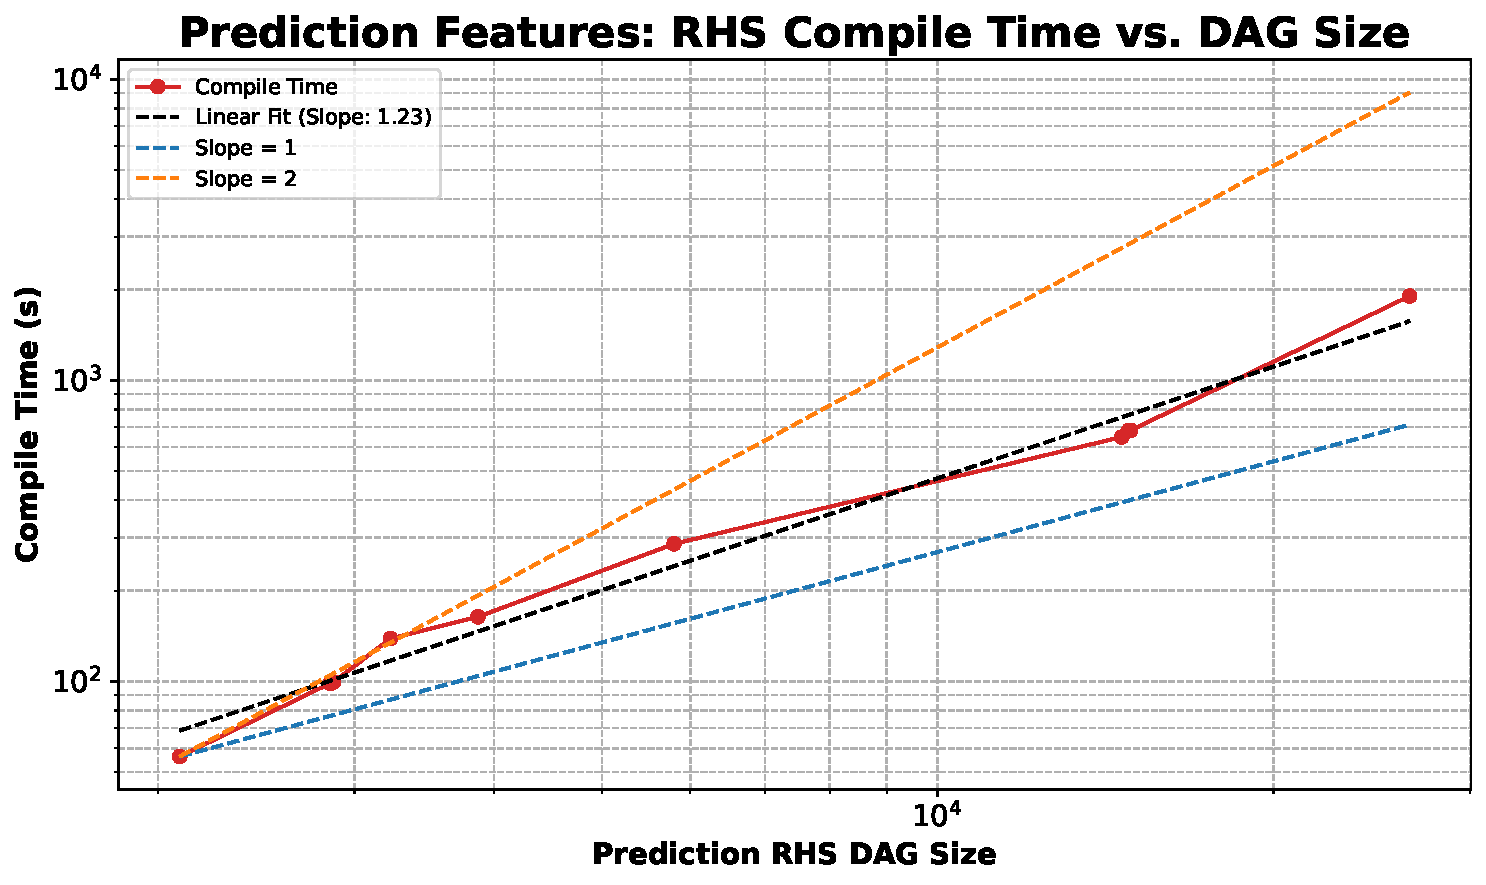
\includegraphics[width=\textwidth]{Figures/mtc/compile_dag_scaling.pdf}
    \end{column}
\end{columns}

\end{frame}

\begin{frame}\frametitle{Big DAG Part 2: Why So Many DV Evaluations?}
\begin{columns}[T, onlytextwidth] % Aligns contents at the top
    \begin{column}{0.48\textwidth}
        \begin{itemize}
          \item Good: Only $332$ nodes per Newton(7sp)
          \item Bad: $>8\times$\texttt{temperature} per RHS
          \begin{itemize}
          \item MFS performs the \texttt{temperature} evals
          \item \texttt{make\_operator\_states} (MOS) is only \textit{partly} responsible
          \item Where are the \texttt{temperature} evals in fluid RHS?:
          \begin{itemize}
          \item myRHS: $1\times$ volume
          \item MOS: $1\times$ quad, $1\times$ per BC ($\text{state}^{-}$), $2\times$ per IEB ($\text{state}^{\pm}$)
          \item $\nabla{T}$, $\nabla{\text{CV}}$: $\le1\times$ per BC ($\text{state}^+$)
          \item CNS: $\le1\times$ per \{inv, visc\} BC ($\text{state}^+$)
          \item Untracked: $\sim1$ superfluous calls?
          \end{itemize}
          \end{itemize}
          \item Worse: BC $\text{state}^+$ splat can't be eliminated (completely)
        \end{itemize}
        %\vspace{10pt}
        %\centering
        %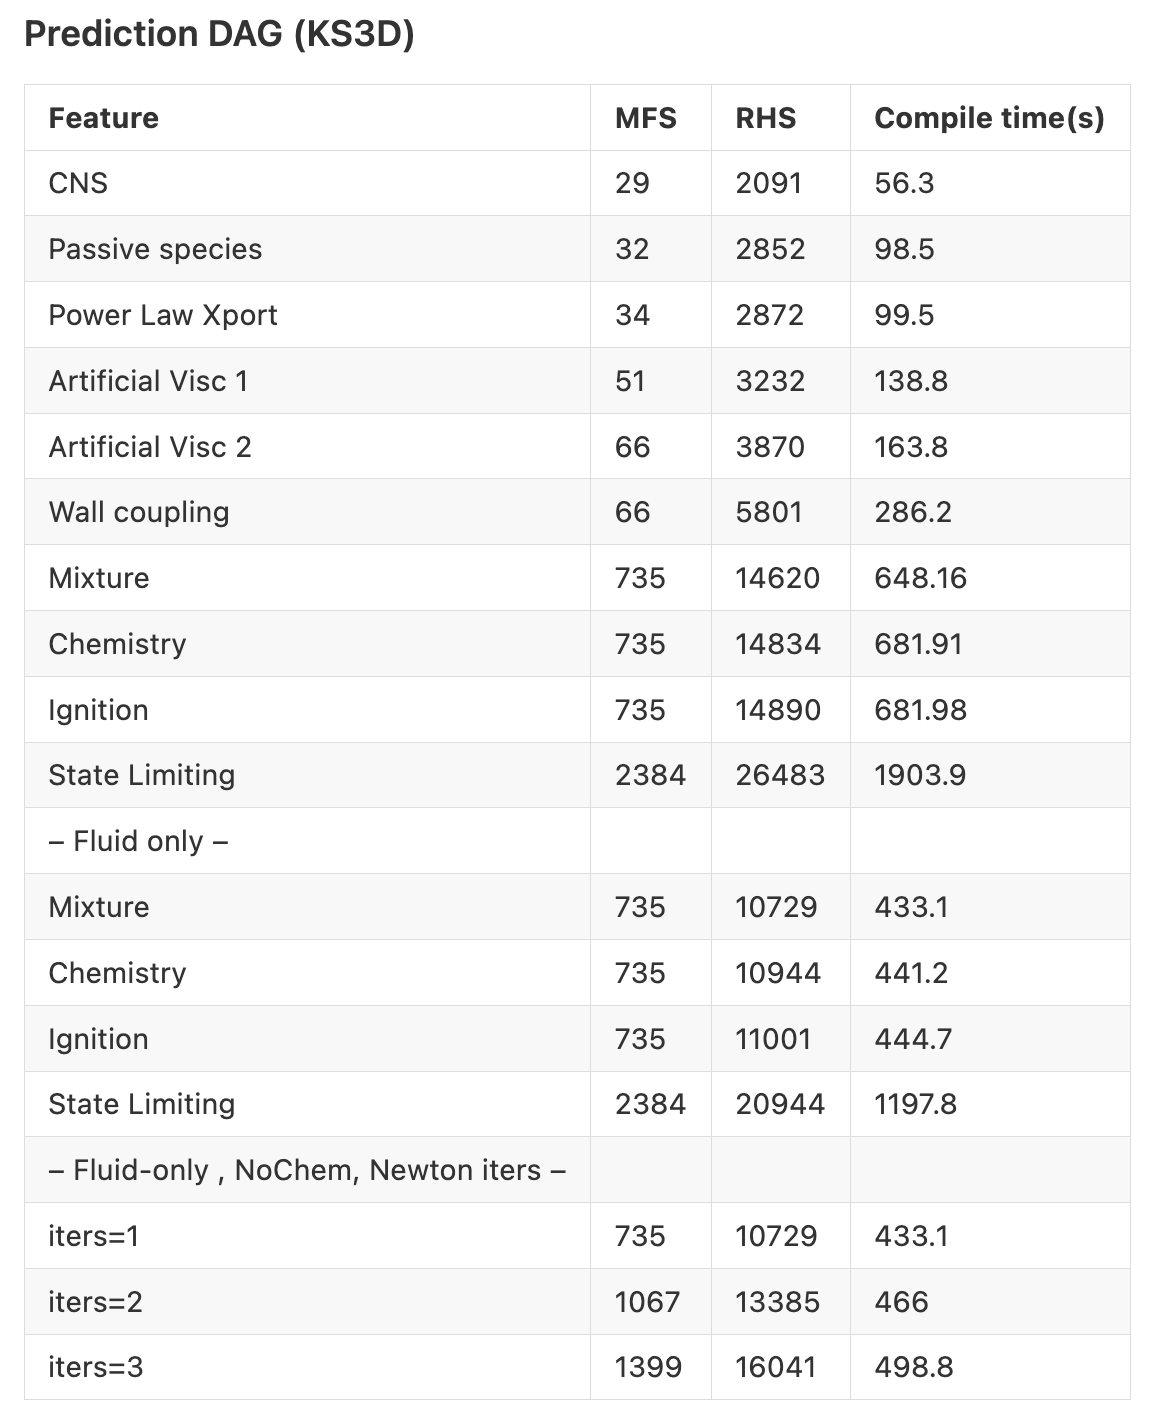
\includegraphics[width=.8\textwidth]{Figures/mtc/prediction_dag_table.png}
        %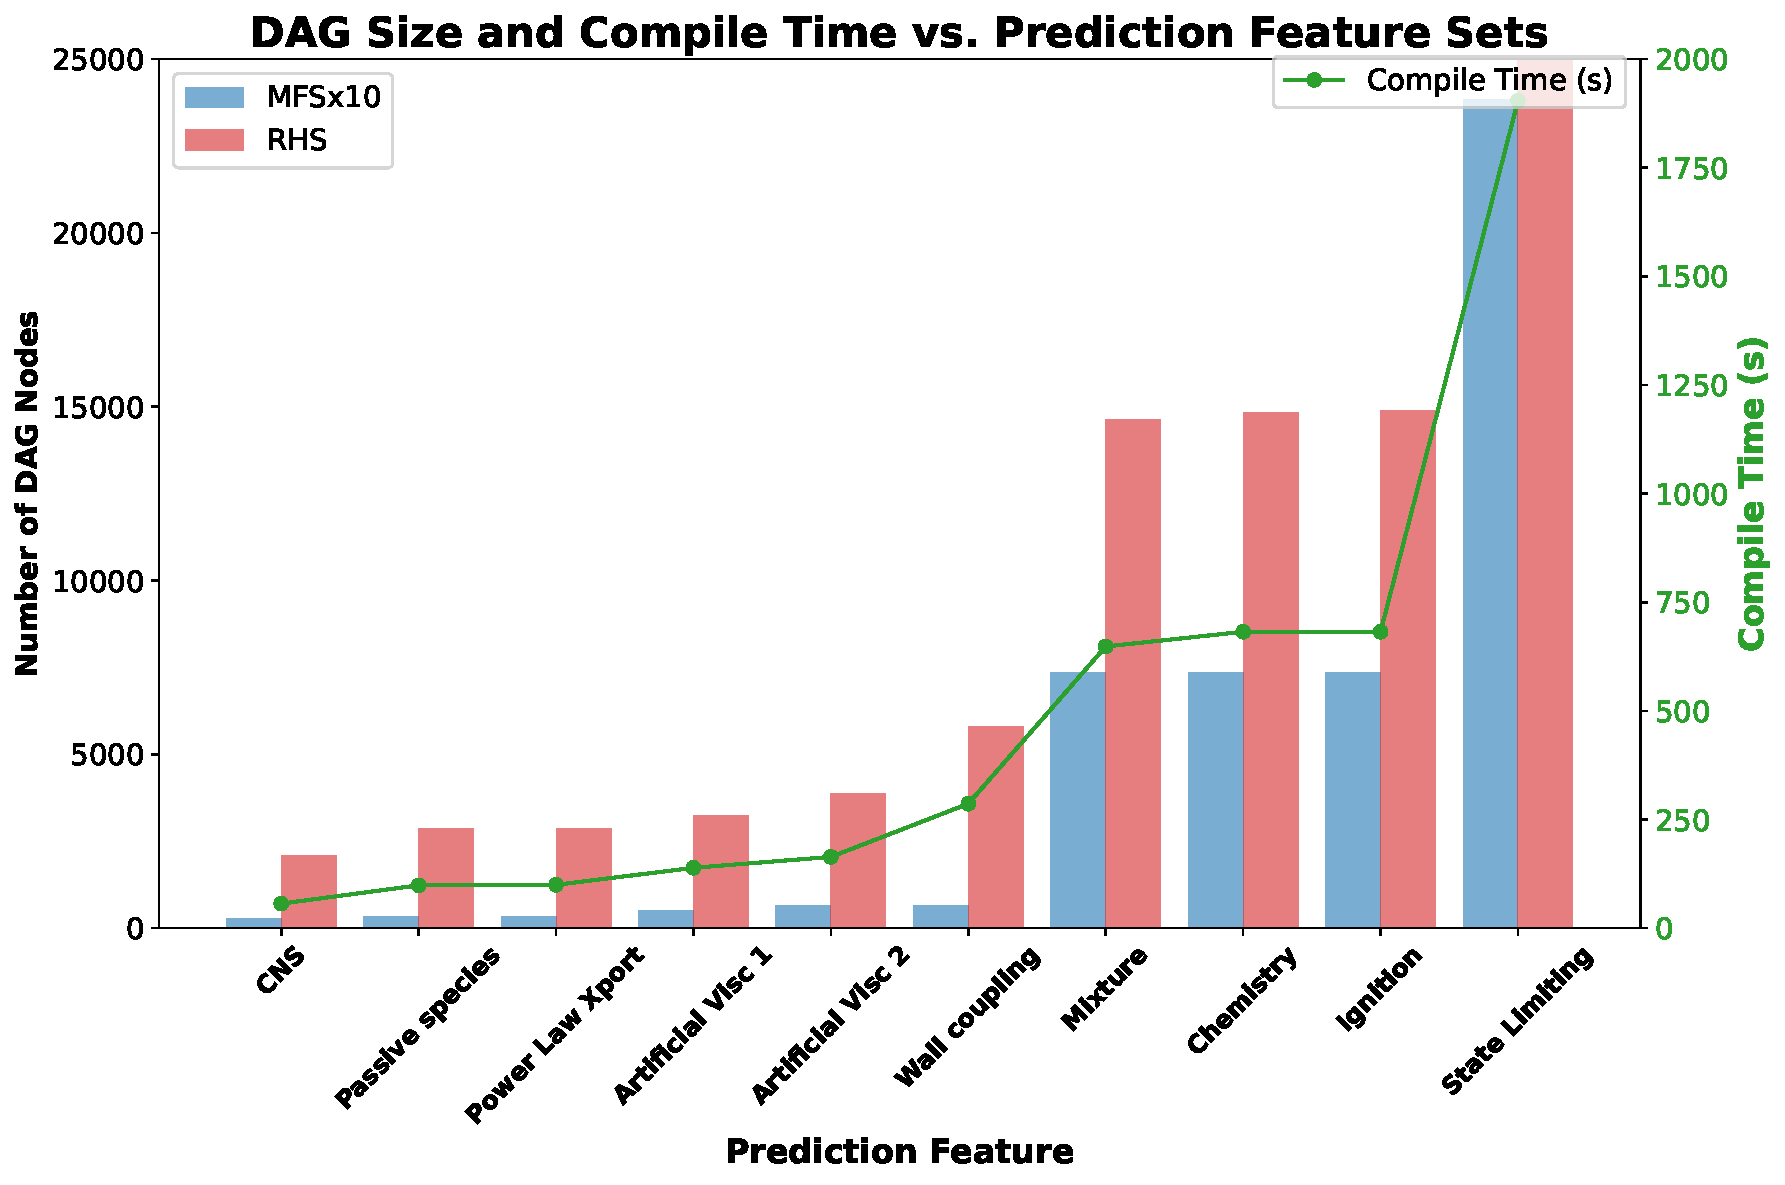
\includegraphics[width=\textwidth]{Figures/mtc/prediction_features_dag.pdf}
    \end{column}
    \begin{column}{0.48\textwidth}
        \vspace{40pt}
        \centering
        \textbf{DAG Counts for KS3D: Gas-only, 7sp}\\
        \vspace{3pt}
        \begin{tabularx}{\textwidth}{|X|X|X|X|X|}
            \hline
            \textbf{Newton} & \textbf{MFS} & \textbf{RHS} & \textbf{Cmp(s)} \\ \hline
            1 & 735 & 10729 & 433 \\ \hline
            2 & 1067 & 13385 & 466 \\ \hline
            3 & 1399 & 16041 & 499 \\ \hline
        \end{tabularx}        
    \end{column}
\end{columns}

\end{frame}

\begin{frame}
    \centering
    \Large
    Next Steps
\end{frame}

\begin{frame}\frametitle{Summary and Next Steps}
\begin{itemize}
\item \mirgecom{} has prediction-supporting performance, but we aren't satisfied
\item First: Eliminate DAG splat with extreme prejudice
\begin{itemize}
\item Matt is closing in on done with function outlining
\item Mike will eliminate extra temperature evaluations by refactoring
\item ``temperature splat'' not very impactful for 7sp, less urgent
\end{itemize}
\item Next: Detailed performance studies
\begin{itemize}
\item DG bakeoff: Scalar advection diffusion?
\begin{itemize}
\item Admits analytic exact solution
\item Exercises non-trivial operators essential to most conservation systems
\item Can craft performance model with relative ease
\end{itemize}
\item Evaluate on varied platforms: Tioga@LC, Delta@NCSA, Aurora@ANL
\end{itemize}
\end{itemize}
%\end{multicols}
\end{frame}

% NO
%
%======================================================================
\begin{frame}\frametitle{}

\vspace*{0.2in}

\begin{center}


\includegraphics[width=0.35\textwidth]{../ceesd-logo-2.pdf}

\vspace*{0.35in}
\cPI{\huge Questions?}

\vspace*{0.5in}
\begin{minipage}{0.6\textwidth}
This material is based in part upon work supported by the Department of Energy, National Nuclear Security Administration, under Award Number DE-NA0003963. 
\end{minipage}



\end{center}


\end{frame}
%======================================================================


%\begin{frame}\frametitle{Symbolic Infrastructure: Fluid Domain Example}
%  \begin{center}
%  %Evolution equation:
%  Compressible Navier--Stokes for reactive mixtures:
%  \begin{equation*}
%    \frac{\partial\mathbf{Q}}{\partial{t}} + \nabla \cdot (\mathbf{F}^I - \mathbf{F}^V) - \mathbf{S} = 0
%  \end{equation*}
%  % With chemistry source terms:
%  % \begin{equation*}
%  %  \mathbf{S} = [ 0, 0, 0, 0, 0, W_k\dot{\omega_k} ]
%  %\end{equation*}
%    Where state vector $\mathbf{Q}$, fluxes $\mathbf{F}^I$, $\mathbf{F}^V$ , and sources $\mathbf{S}$ are given by:
% \begin{equation*}
%      \begin{bmatrix}
%        \rho\\\rho{E}\\\rho\vec{v}\\\rho{Y}_\alpha\end{bmatrix},\quad
%      \begin{bmatrix} \rho\vec{v}\\(\rho{E} +
%        p)\vec{v}\\\rho(\vec{v} \otimes \vec{v}) +
%        p\delta_{ij}\\\rho{Y}_\alpha\vec{v}\end{bmatrix}, \quad
%       \begin{bmatrix} 0\\(\mathbf{\tau} \cdot \vec{v} - \mathbf{q})\\\mathbf{\tau}\\-\mathbf{J}_\alpha\end{bmatrix},\quad
%       \begin{bmatrix} 0\\0\\0\\W_\alpha\dot{\omega}_\alpha\end{bmatrix}
% \end{equation*}
% $\tau = \mu\left(\nabla\vec{v} + (\nabla\vec{v})^T\right) + \left(\mu_b - \frac{2\mu}{3}\right)\left(\nabla \cdot \vec{v}\righ%t)$\\
%\vspace{5pt}
%$\mathbf{J}_\alpha = -\rho D_{(\alpha)} \nabla(Y_\alpha)$ \quad and \quad $\mathbf{q} = -\kappa\nabla{T} + h_\alpha\mathbf{J}_\%alpha$\\
%\vspace{10pt}
%    The mixture gas model (EOS) provides $\rightarrow~~(p,T,e,\mu,\kappa,D_{\alpha}, \omega_\alpha, h_\alpha)(\mathbf{Q})$
%  \end{center}
%  \begin{tikzpicture}[remember picture, overlay]
%    \fill <2> [fill=white, opacity=0.8] (current page.south west) + (0.5,0.5) rectangle (12.5,7.5);
%    \node <2> [inner sep=0pt] at (current page.center) {
%      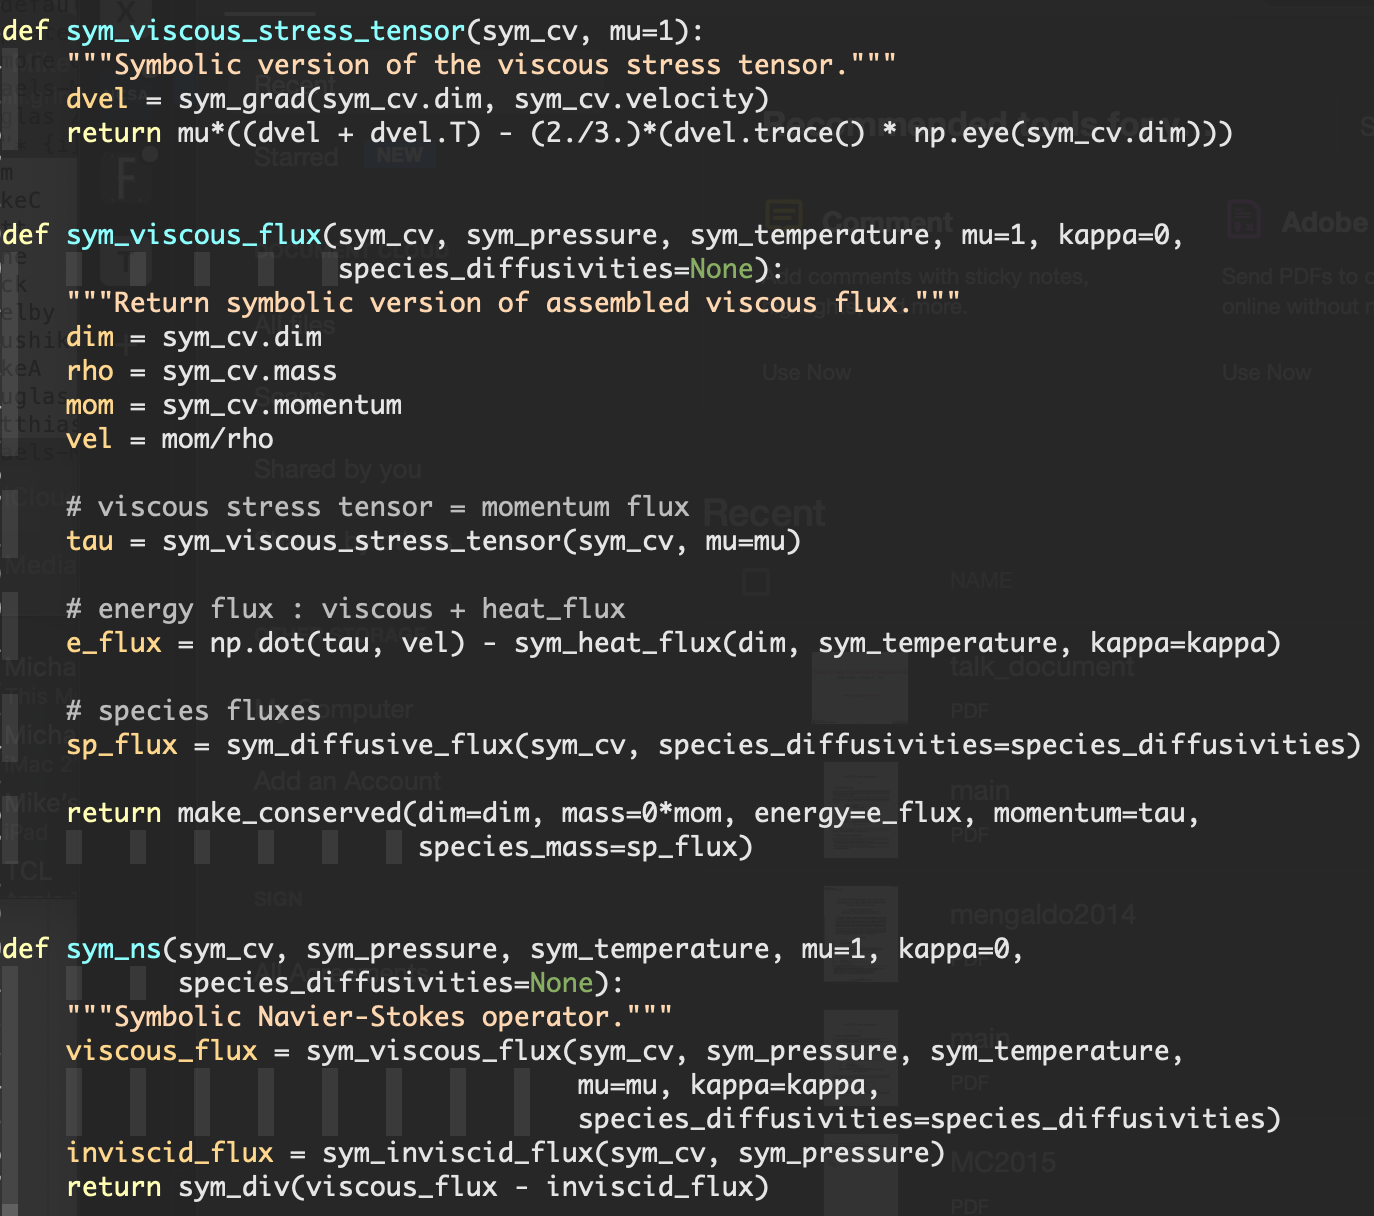
\includegraphics[width=.5\textwidth]{Figures/mtc/SymbolicInfrastructureCode.png}
%    };
%  \end{tikzpicture}
%\end{frame}
%
%\begin{frame}\frametitle{Component Testing With Symbolic Infrastructure}
%% \center{What's it good for?}
%\begin{itemize}
%\item Fluid component verification testing
%\item Specify analytic test functions and 
%\item Evaluate convergence of MIRGE components to exact/analytic solution
%\end{itemize}
%\begin{center}
%  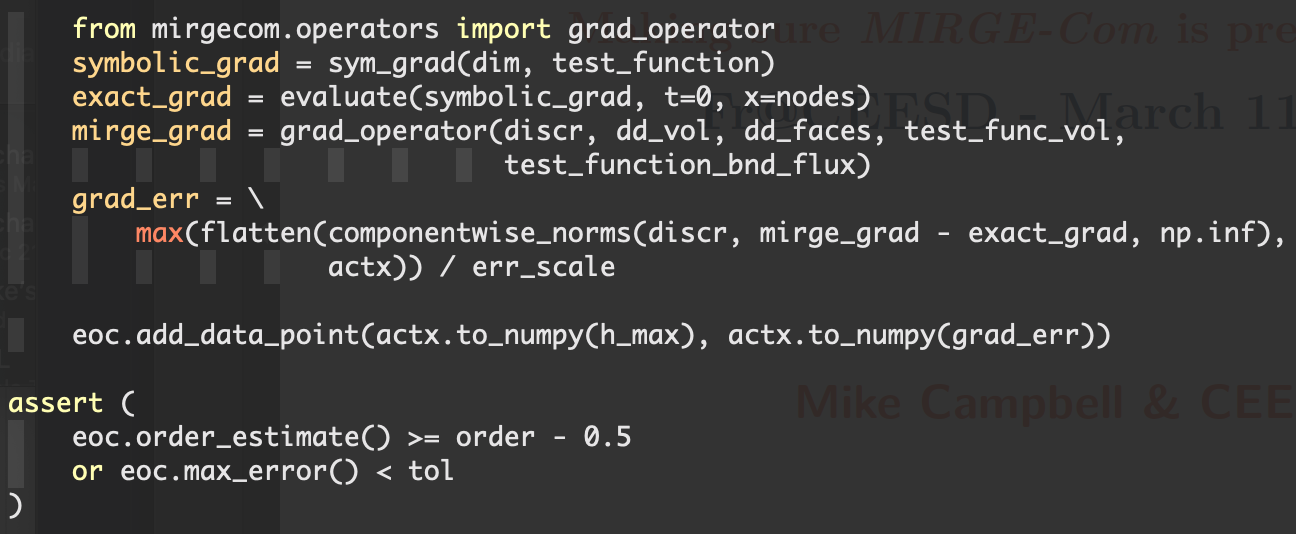
\includegraphics[width=.6\textwidth]{Figures/mtc/ComponentVerifCode.png}
%\end{center}
%\begin{itemize}
%\vspace{-10pt}
%\item and ... method of manufactured solutions (MMS)
%\end{itemize}
%\end{frame}


%\begin{frame}\frametitle{Monitoring Daily Y3 Tests on Lassen}
%\begin{minipage}[t][0.3\textheight][t]{\textwidth}
%\begin{center}
%https://github.com/illinois-ceesd/timing
%\end{center}
%\begin{multicols}{2}
%\begin{itemize}
%\item Data on key capabilities collected nightly
%\item Intended to track performance vs. code/features
%\item $\Delta$'s indicate change in performance
%\columnbreak
%\item New this cycle:
%\begin{itemize}
%\item Multi-case/comparitive plotting
%\item Tracking parallel cases
%\end{itemize}
%\end{itemize}
%\end{multicols}
%\end{minipage}\vfill
%\begin{center}
%  % 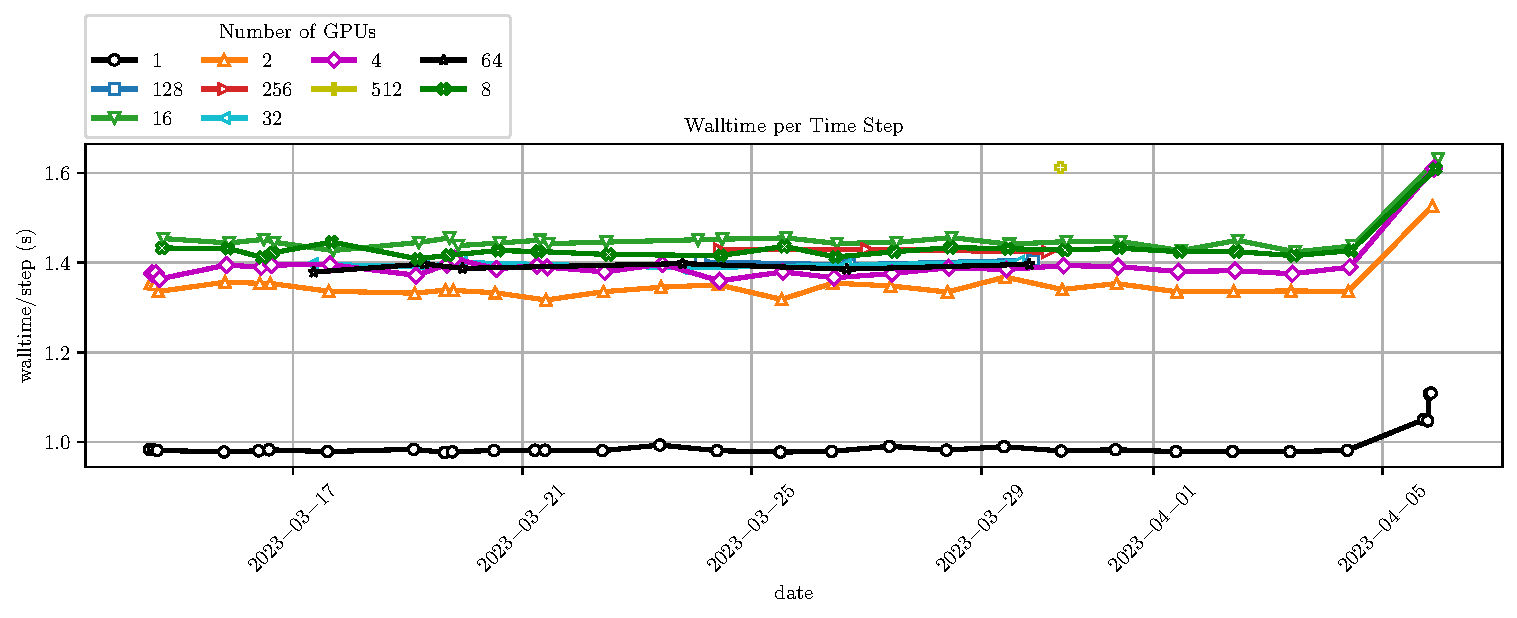
\includegraphics[width=.8\textwidth]{Figures/mtc/y3-prediction-parallel-20230405.pdf}
%  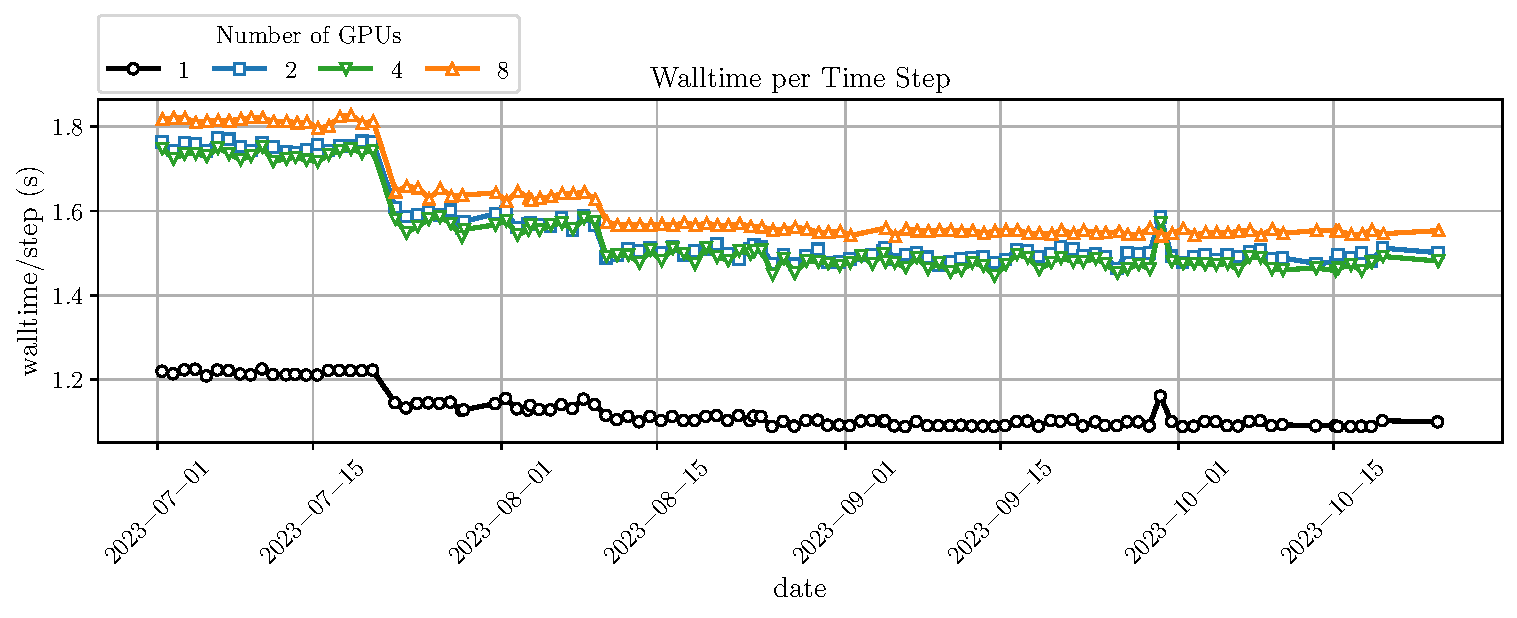
\includegraphics[width=.8\textwidth]{Figures/mtc/parallel_history_2nodes.pdf}
%\end{center}
%\end{frame}

%\begin{frame}\frametitle{CNS Verification with MMS}
%  \begin{multicols}{2}
%  \begin{itemize}
%  \item Integrated MMS: Roy Solution
%  \item 2,3 dimensions, sub/super-sonic
%  \item Exact boundaries
%  \item Exercises all CNS equations (single gas)
%  \end{itemize}
%  \begin{center}
%  \vspace*{-5pt}
%  \tiny{Roy MMS components}
%  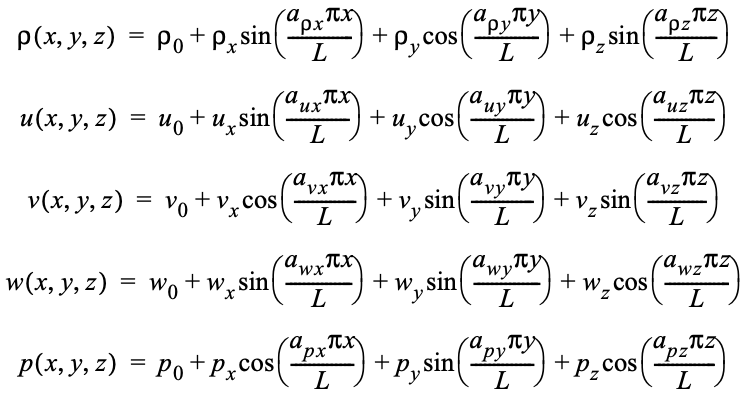
\includegraphics[width=.4\textwidth]{Figures/mtc/RoySoln.png}
%  \end{center}
%  \columnbreak
%  \vspace*{-35pt}
%  \begin{center}
%  \tiny{Pressure contours for 3D subsonic Roy MMS.}
%  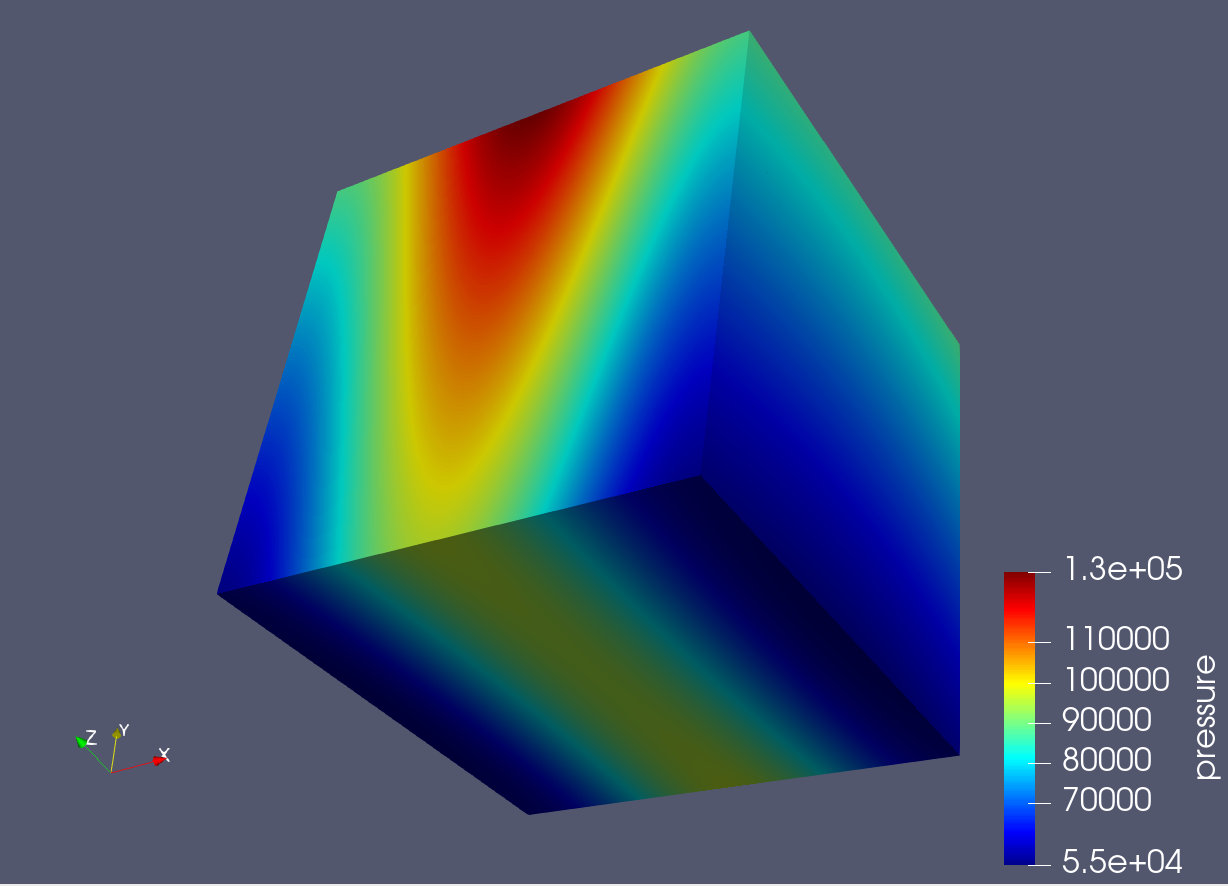
\includegraphics[width=.3\textwidth]{Figures/mtc/RoyPressure3D.png}\\
%  \vspace*{10pt}
%  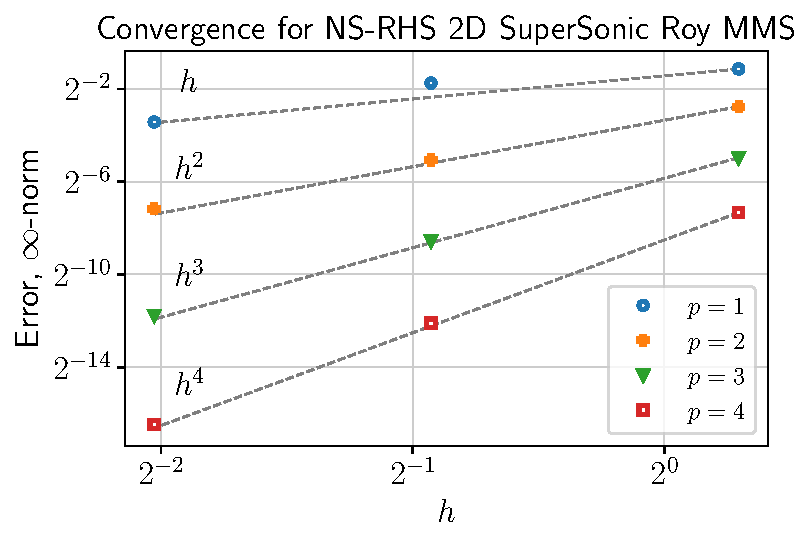
\includegraphics[width=.35\textwidth]{Figures/mtc/roy_convergence.pdf}
%  \end{center}
%  \end{multicols}
%  \begin{center}
%  \vspace*{-10pt}
%  \begin{minipage}{.8\textwidth}
%  \paper{\sPI{C.~Roy, T.~Smith, and C.~Ober}, ``Verification of a Compressible CFD Code using the Method of Manufactured Solutions,'' \textit{AIAA} Paper 2002-3110 (2002)}
%  \end{minipage}
%  \end{center}
%\end{frame}

%\begin{frame}\frametitle{Thermochemistry Verification in \mirgecom}
%\begin{center}
% Autoignition co-verification
%\end{center}
%\begin{itemize}
%   \item Ethylene/air mixture $(1500\mathtt{K}, \rho=\mathtt{const})$
%   \item \pyrometheus-predicted profiles match \textit{Cantera}
%   \item \pyrometheus{} with implicit time integration with \textit{CVODE}
%   \item \mirgecom{} with RK4, inviscid, quiescent
%\end{itemize}
%\begin{multicols}{2}
%    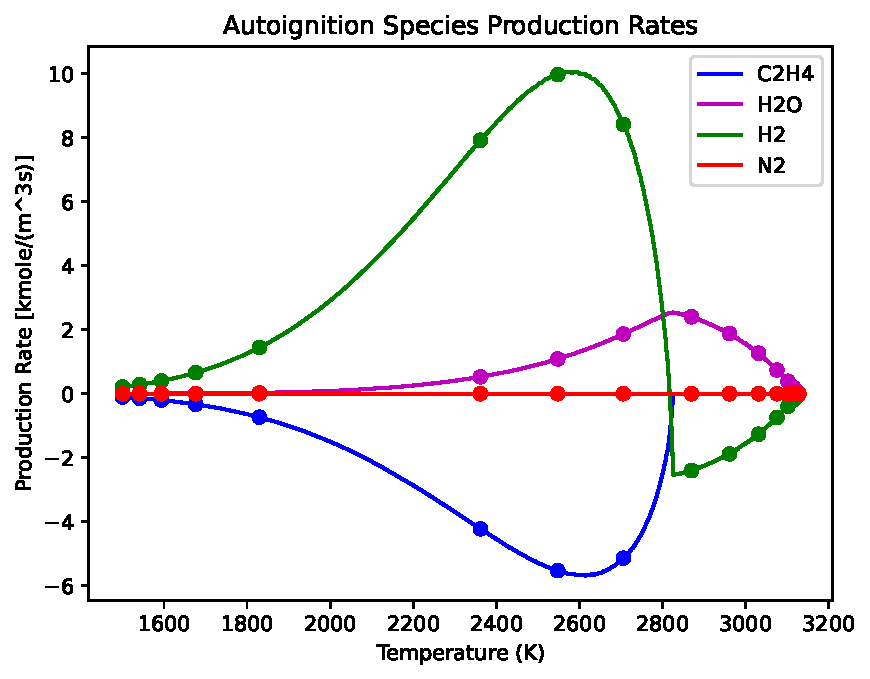
\includegraphics[width=.4\textwidth]{Figures/mtc/autoignition_rates.pdf}\\
%    \columnbreak
%    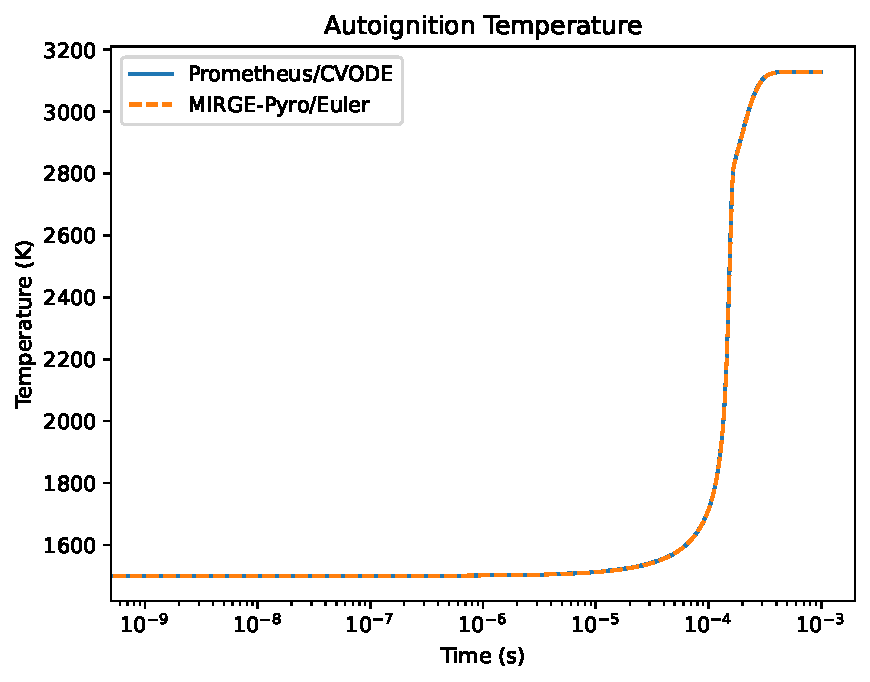
\includegraphics[width=.4\textwidth]{Figures/mtc/autoignition_temperature.pdf}
%  \end{multicols}
%\end{frame}

%\begin{frame}\frametitle{Performance Monitoring on Lassen}
%\begin{minipage}[t][0.3\textheight][t]{\textwidth}
%\begin{center}
%https://github.com/illinois-ceesd/timing
%\end{center}
%\begin{multicols}{2}
%\begin{itemize}
%\item Data on key capabilities collected nightly
%\item Intended to track performance vs. code/features
%\item $\Delta$'s indicate change in performance
%\columnbreak
%\item New this cycle:
%\begin{itemize}
%\item Multi-case/comparitive plotting
%\item Tracking parallel cases
%\end{itemize}
%\end{itemize}
%\end{multicols}
%\end{minipage}\vfill
%\begin{center}
%  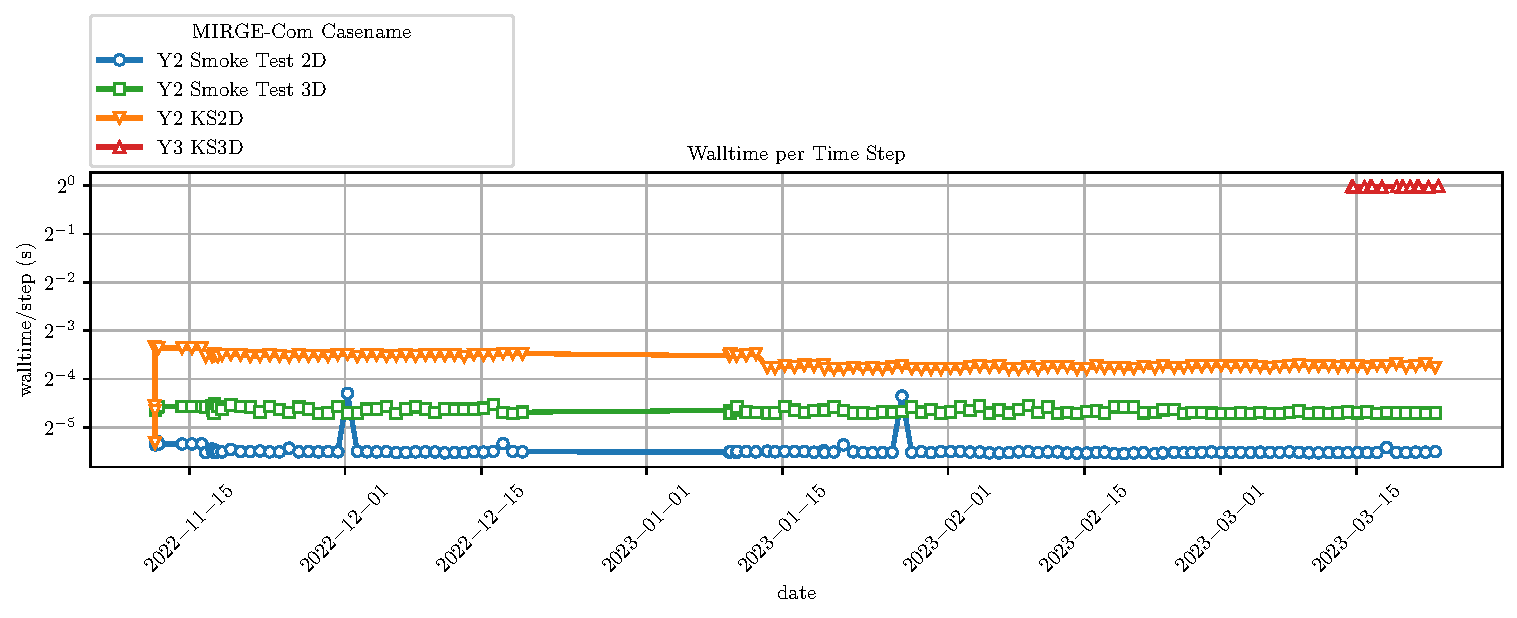
\includegraphics[width=.8\textwidth]{Figures/mtc/multicase_step.pdf}
%\end{center}
%\end{frame}

%\begin{frame}\frametitle{Performance Monitoring on Lassen}
%\begin{minipage}[t][0.3\textheight][t]{\textwidth}
%\begin{center}
%https://github.com/illinois-ceesd/timing
%\end{center}
%\begin{multicols}{2}
%\begin{itemize}
%\item Data on key capabilities collected nightly
%\item Intended to track performance vs. code/features
%\item $\Delta$'s indicate change in performance
%\columnbreak
%\item New this cycle:
%\begin{itemize}
%\item Multi-case/comparitive plotting
%\item Tracking parallel cases
%\end{itemize}
%\end{itemize}
%\end{multicols}
%\end{minipage}\vfill
%\begin{center}
%  %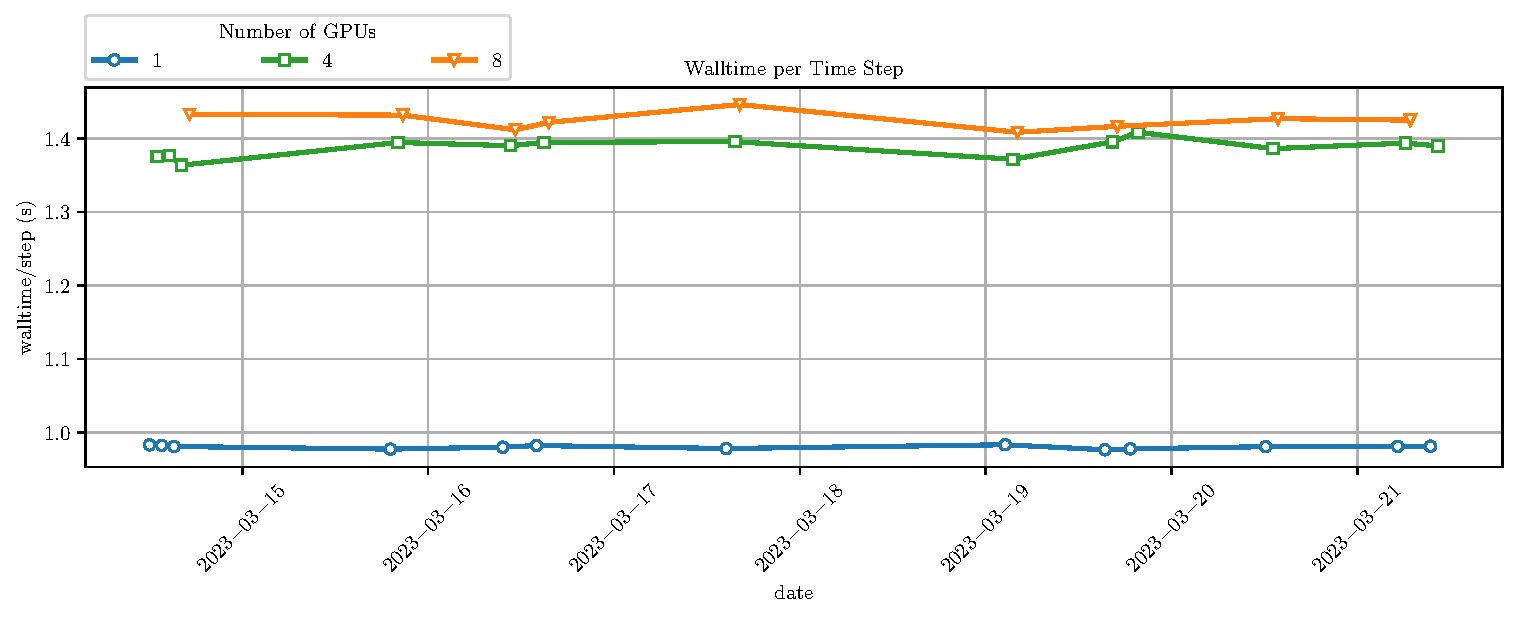
\includegraphics[width=.8\textwidth]{Figures/mtc/prediction-scaling-tracking.pdf}
%  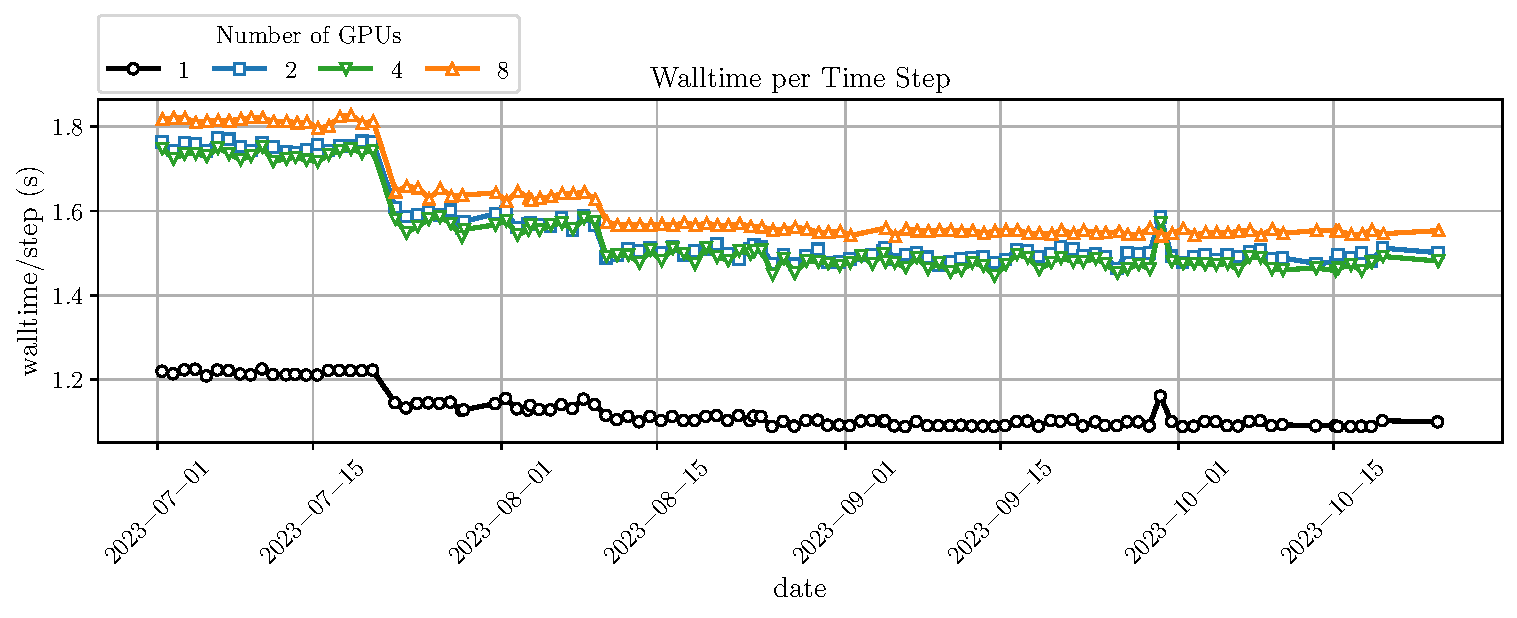
\includegraphics[width=.8\textwidth]{Figures/mtc/parallel_history_2nodes.pdf}
%\end{center}
%\end{frame}


%\begin{frame}\frametitle{Performance \& Scalability - Mesh Scale Testing}
%\begin{minipage}[t][0.45\textheight][t]{\textwidth}
%\begin{center}
%New: prediction-enabling performance
%\end{center}
%\begin{multicols}{2}
%  \begin{itemize}\setlength{\itemsep}{0.02in}
%  \item Linear with number of elements
%  \item Small problems are expensive (performance floor, enqueue times)
%  \item Should strong scale in linear regime
%  \end{itemize}
%  \columnbreak
%  \begin{itemize}\setlength{\itemsep}{0.02in}
%  \item Do not exceed device memory
%    \begin{itemize}
%    \item OOM: Resolved SVM/Unified mem
%    \item Acute performance drag
%    \end{itemize}
%  \item Mem growth: garbage collection \prj{\tiny}{M.~Diener}
%  %\item Memory growth during stepping eventually leads to OOM
%  %\item OOM errors resolved through SVM/Unified memory % \prj\tiny{07c, M.~Diener}
%  %\item Exceeding device mem now spills over (expensively) to host mem
%  %\item Mem growth: resolved through garbage collection
%  \end{itemize}
%%\item Absolute performance could be better
%%\item Recent focus: memory growth
%%\end{itemize}
%\end{multicols}
%\end{minipage}
%\vfill
%\vspace{-30pt}
%\begin{minipage}[t][0.45\textheight][t]{\textwidth}
%\centering
%%Grid Scaling\\
%%\end{center}
%%\begin{center}
%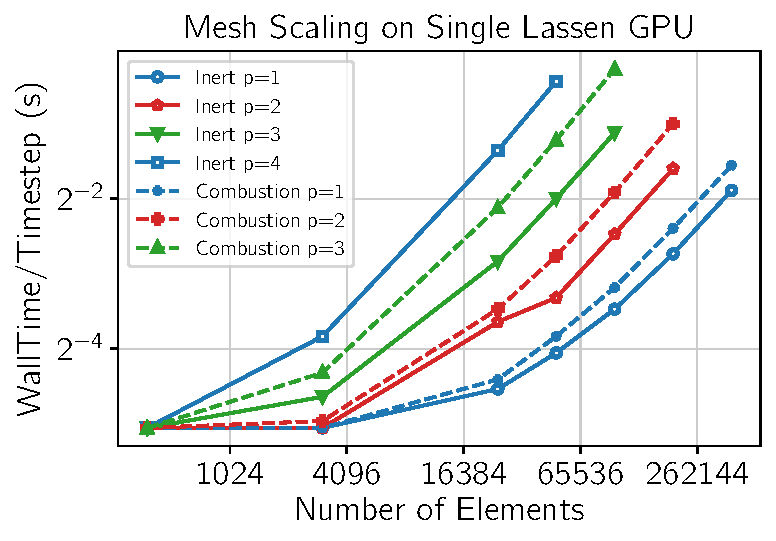
\includegraphics[width=.4\textwidth]{Figures/mtc/combozzle_gridscale.pdf}\hspace{30pt}
%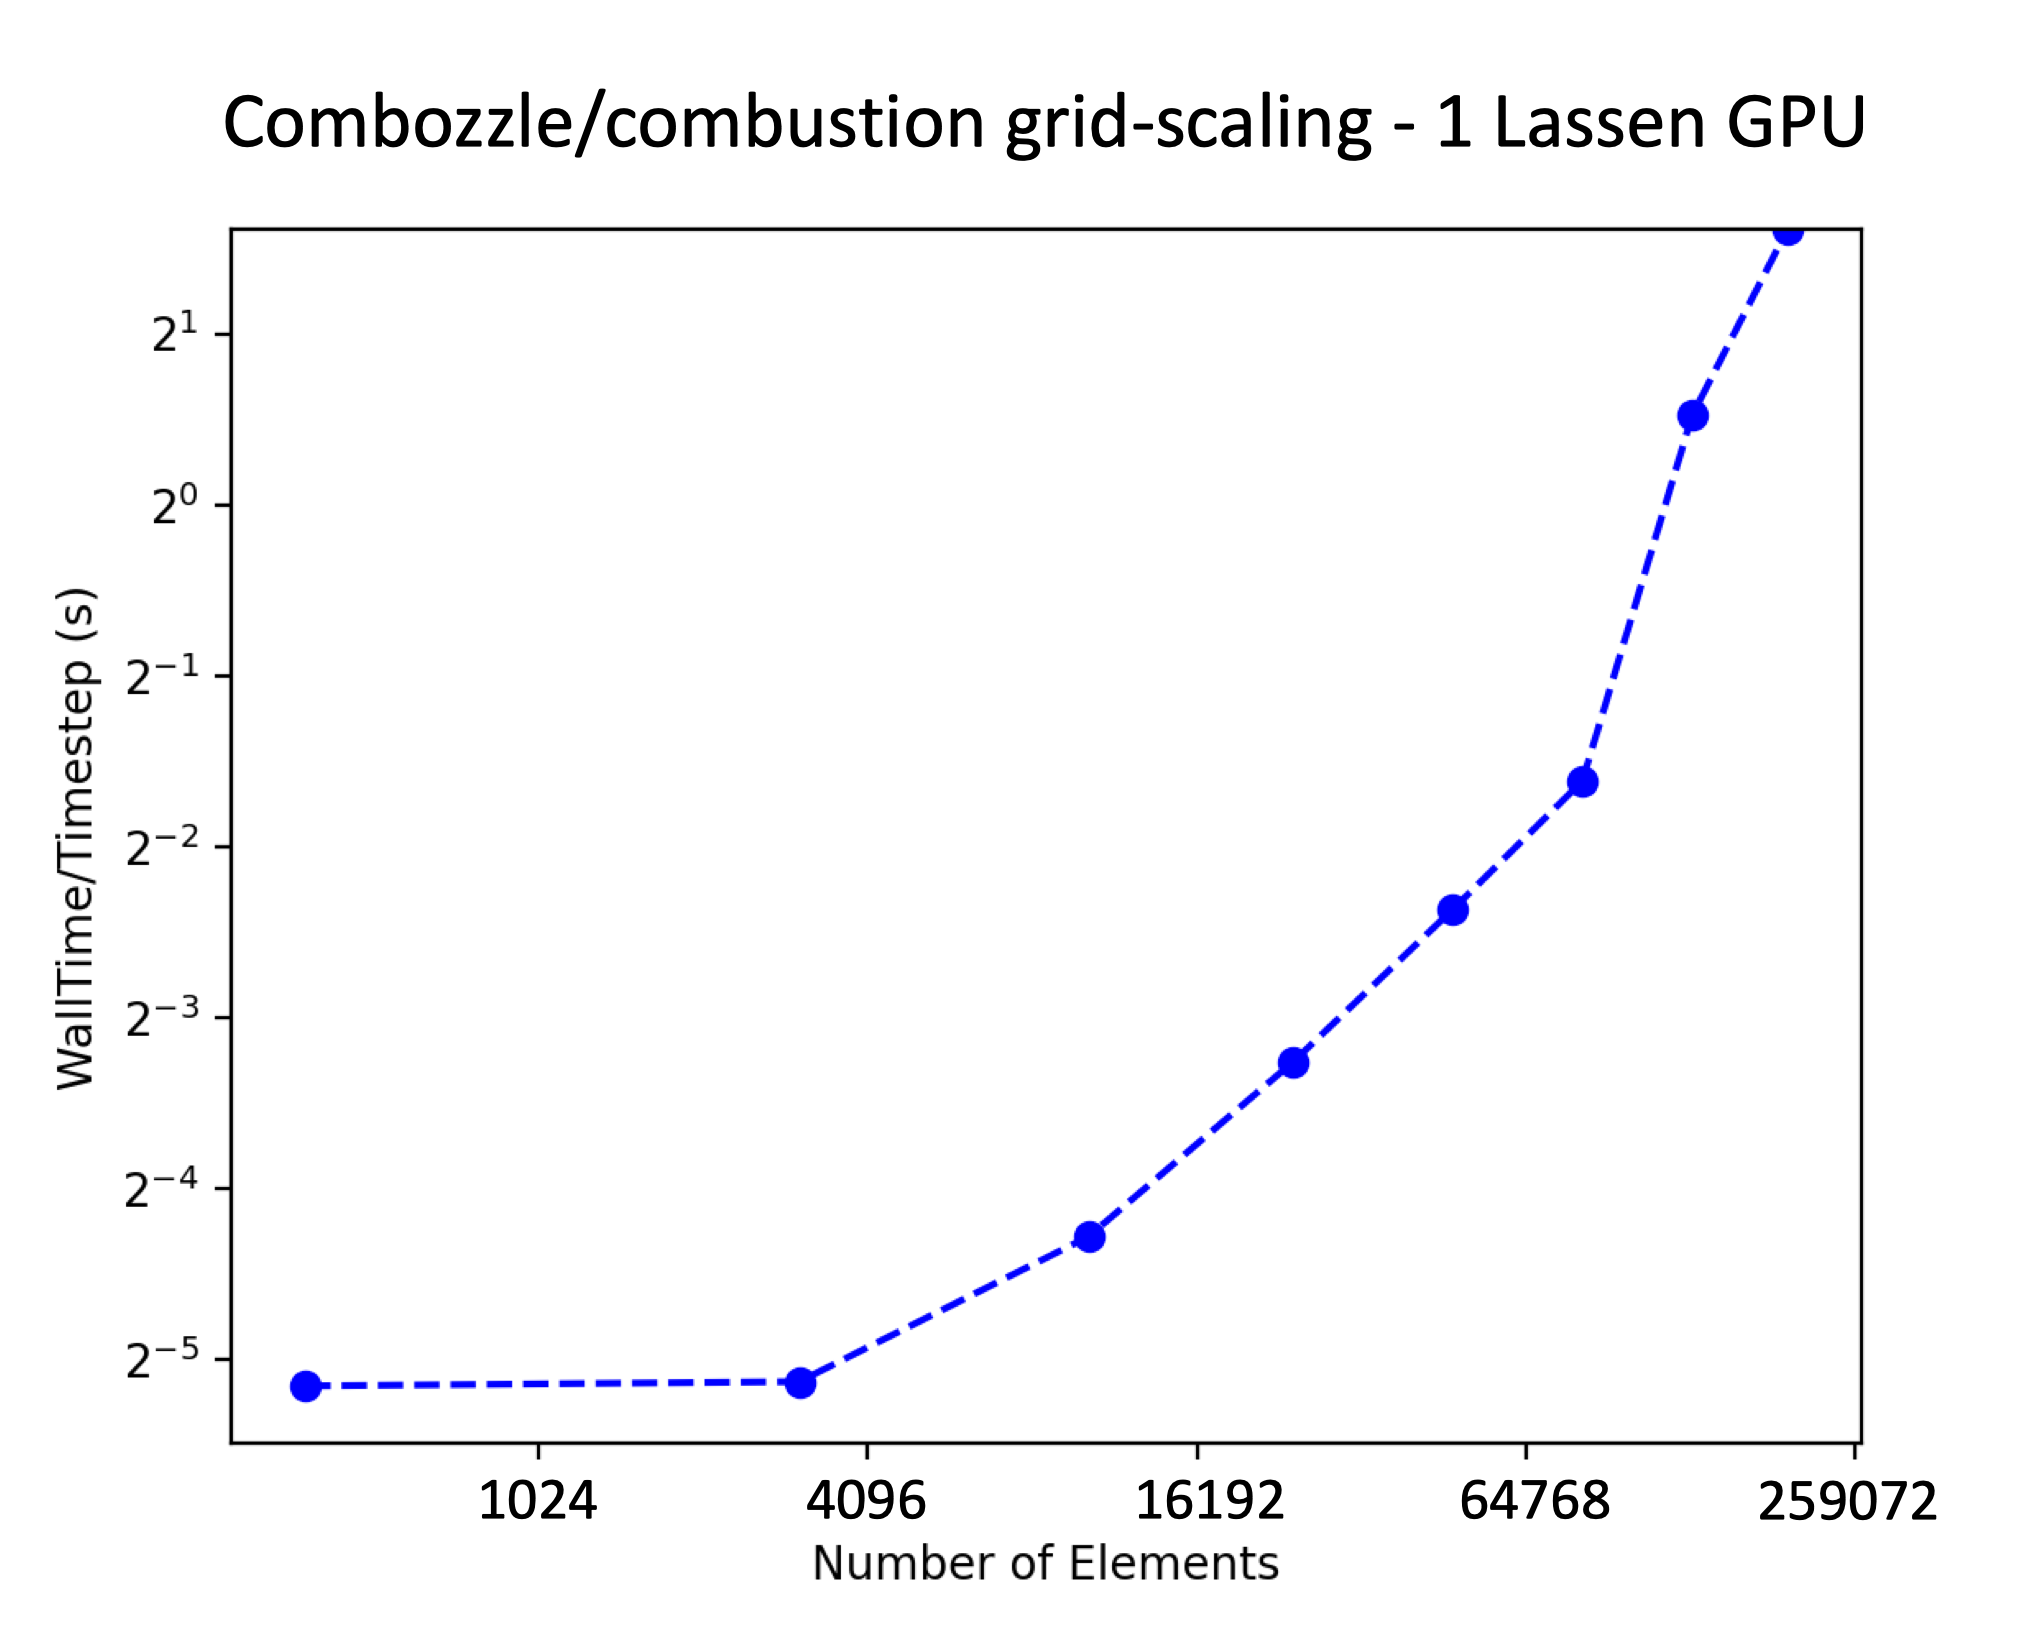
\includegraphics[width=.4\textwidth]{Figures/mtc/comboz_gridscale_svm.png}
%\end{minipage}
%\end{frame}

%\item Computational performance: Speed or FLOPS
%% VS. the machine itself, vs. expectation
%\item Parallel performance: Scalability or efficiency
%\begin{itemize}
%\item Strong scaling: Fixed problem size, scaling resources
%\item Weak scaling: Fixed work/resource, scaling problem size with resource
%\item Mesh scaling: Scaling work, fixed resource
%\end{itemize}
%\item I/O and memory performance: Bandwidth, bytes/second
%\item Cost performance
%\begin{itemize}
%\item Energy efficiency
%\item Total time to solution (TTS)
%\item FLOPS/Fidelity
%\item Usability/Productivity
%\end{itemize}
%\item Why should we care about scalability? (enables prediction!)
%\begin{itemize}
%\item Weak scaling out to prediction-scale
%\item Versatility, portability, and resource options
%\end{itemize}

%\begin{frame}\frametitle{Recall: DAG Splat Effect}
%  \begin{minipage}{0.45\textwidth}		
%    \begin{itemize}
%    \item Fluid-only prediction-like physics (no wall model, boundaries)
%    \item 3D, periodic, 3rd order elements
%    \item Weak scaling with 48k elements/GPU (1 rank/GPU)
%    \end{itemize}
%    \begin{center}
%    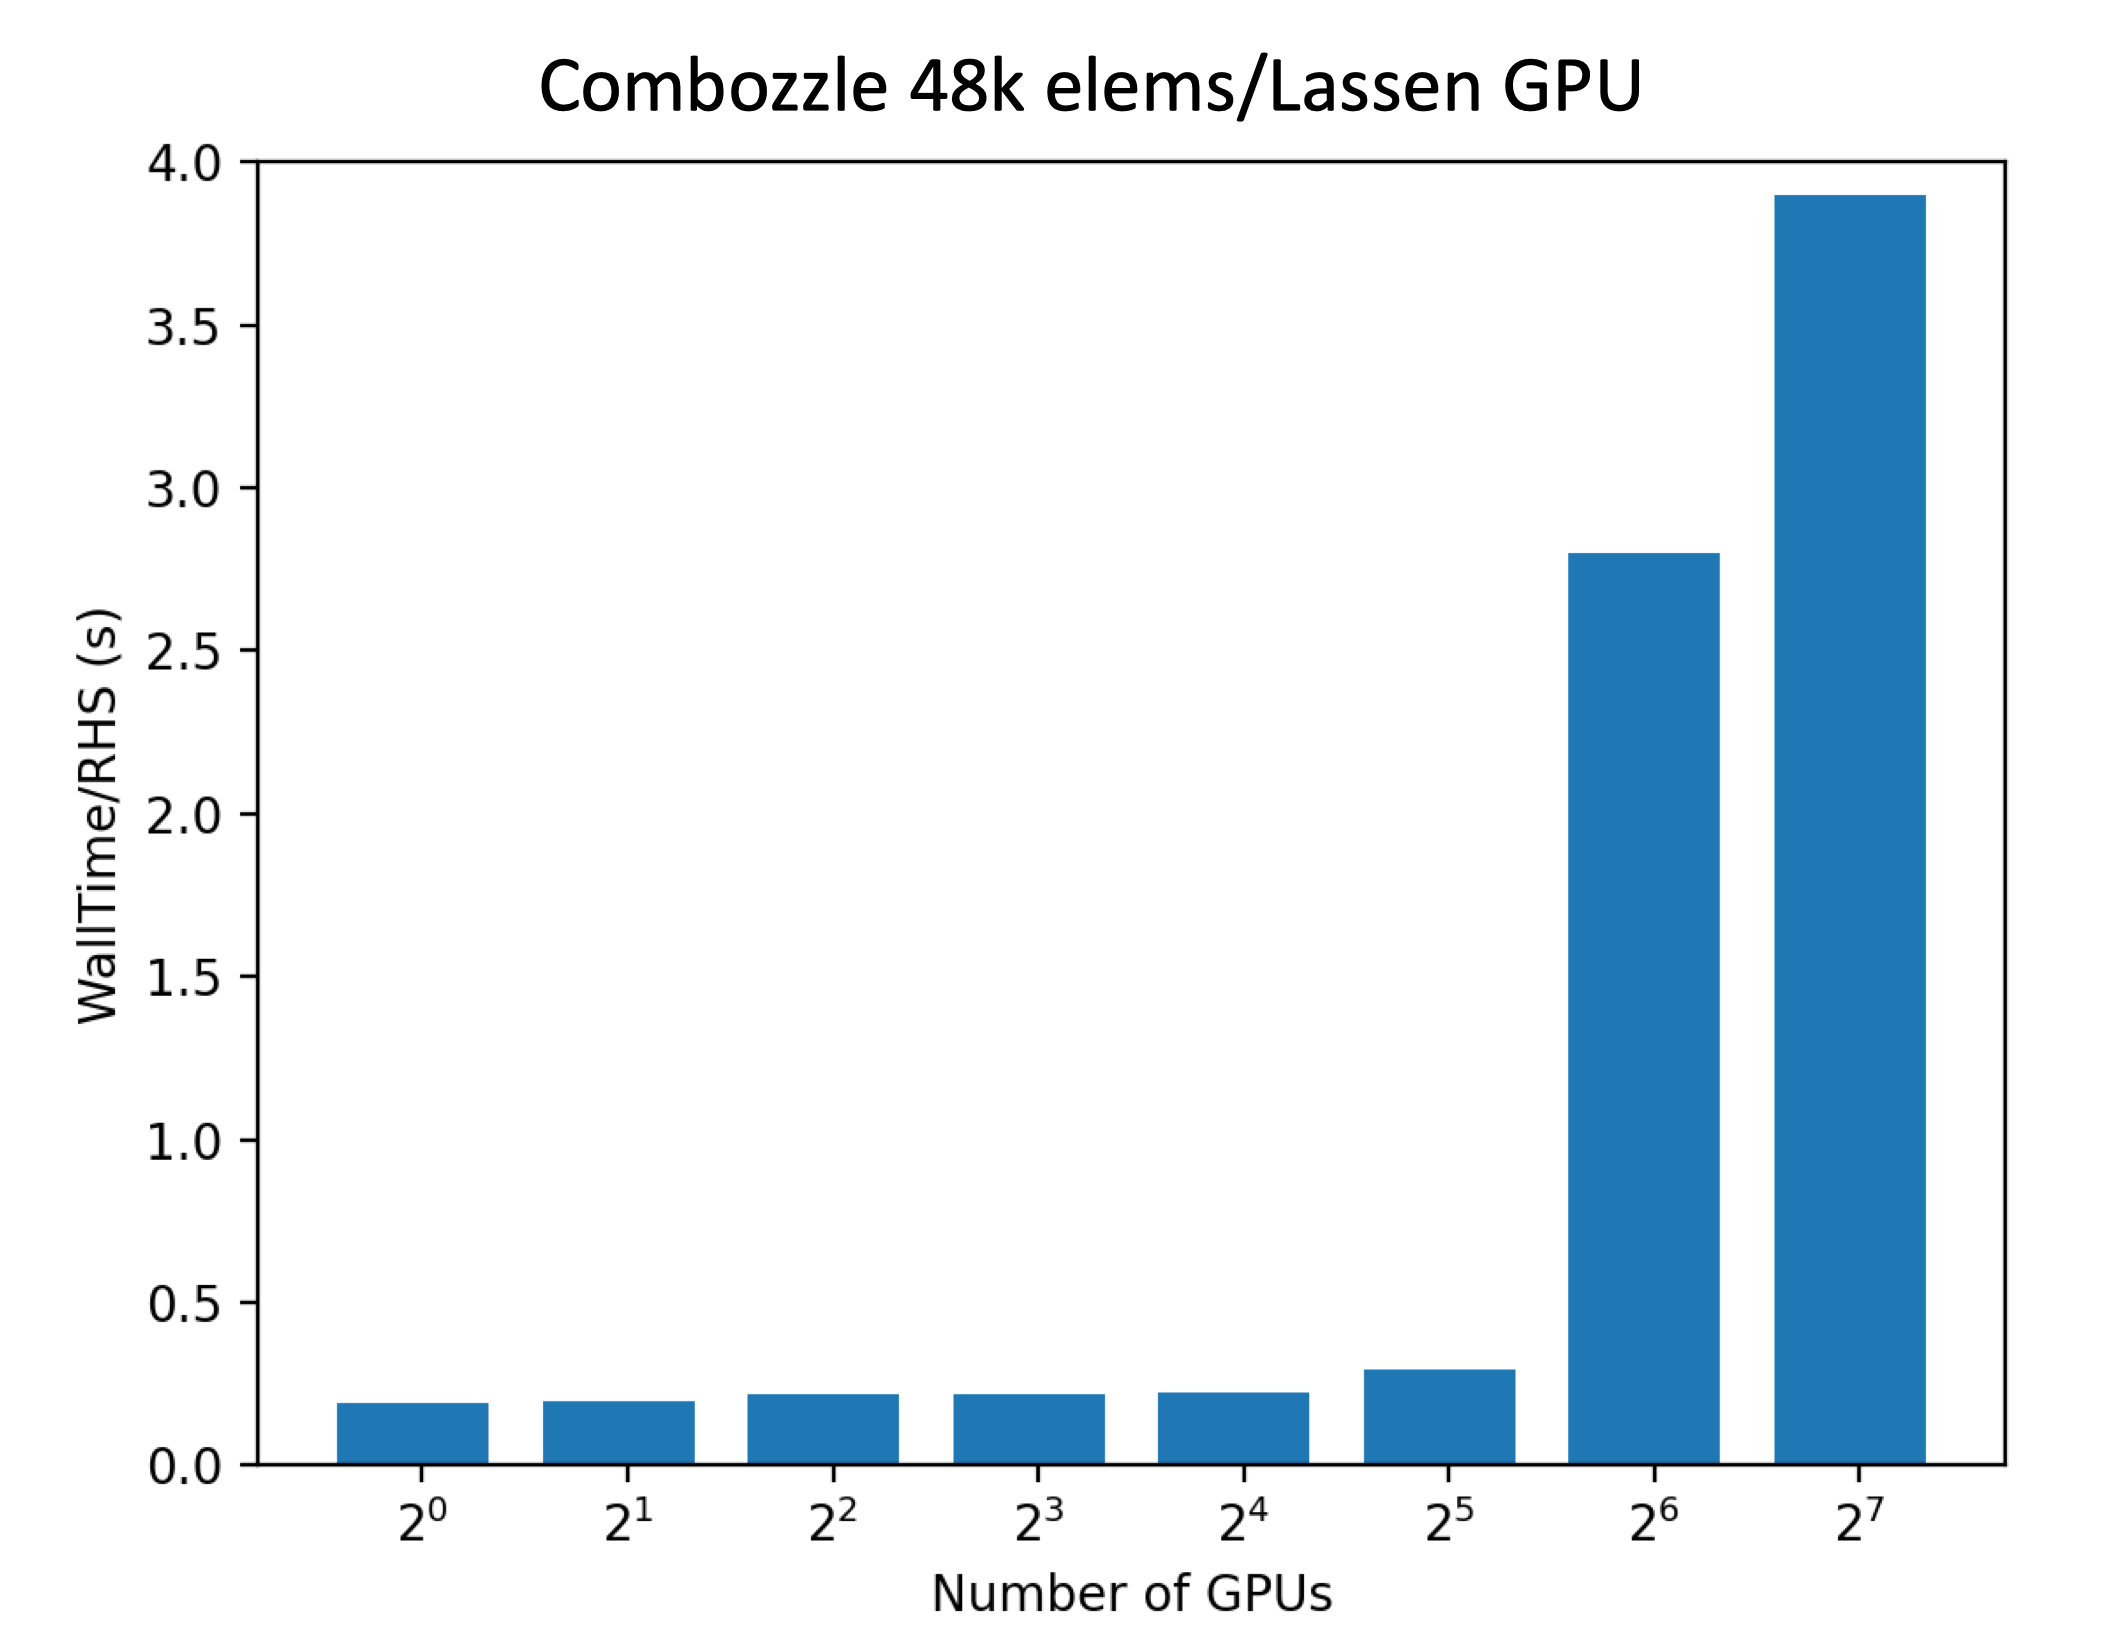
\includegraphics[width=.8\textwidth]{Figures/mtc/combozzle_weak_bad_partitioning.png}
%    \end{center}
%  \end{minipage}
%  \begin{minipage}{0.5\textwidth}
%    \begin{figure}
%      \centering
%      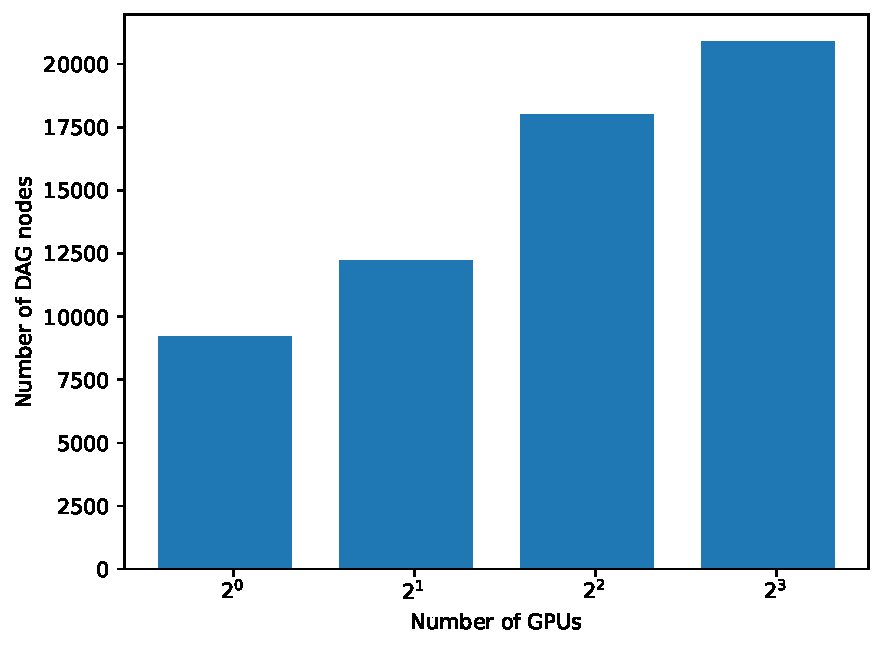
\includegraphics[width=.6\textwidth]{Figures/mtc/dag_scaling.pdf} \\
%      \vspace{2pt}
%      \begin{itemize}
%      \item Anomalous behavior > 32 GPU
%      \item Surprising DAG scaling
%      \item DAG splat (function DAG inlining):
%      \begin{itemize}
%      \item Flux \& DV DAG at each boundary; BCs and inter-element (IEB)
%      \item Function \texttt{make\_fluid\_state} (MFS): Limiting, DV
%      \item Mixture temperature update DAG at every Newton iteration
%      \end{itemize}
%      \end{itemize}
%    \end{figure}		
%  \end{minipage}
%\end{frame}

%\begin{frame}\frametitle{Recall: Addressing DAG Splat}
%  \begin{minipage}{0.45\textwidth}		
%  %\vspace{10pt}
%    \begin{itemize}
%    \item DAG splat mitigation:
%    \begin{itemize}
%    \item 1D part; particle board $\rightarrow$ pancakes
%    \item Unlocks prediction-scale: 25M elems (6B DOFs)/512 GPUs
%    \end{itemize}
%    \item DAG splat solutions:
%    \begin{itemize}
%    \item Application: refactor MFS 
%    \item Infrastructure: function outlining \prj{\tiny}{M.~Smith}
%    \end{itemize}
%    \end{itemize}
%    \begin{center}
%    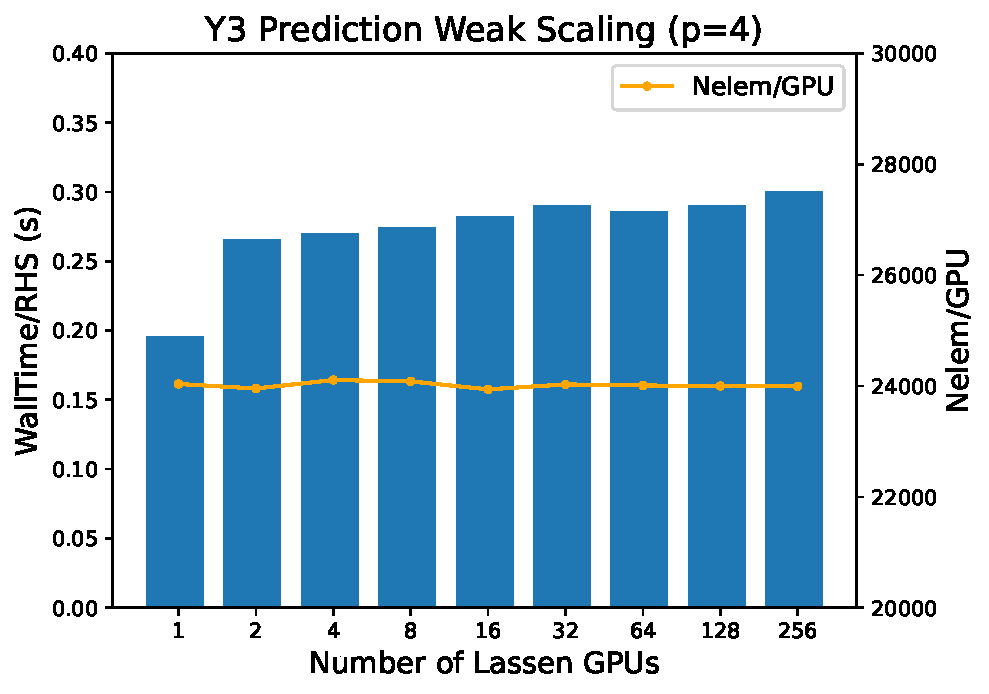
\includegraphics[width=.8\textwidth]{Figures/mtc/y3-prediction_weak_scaling.pdf}
%    \end{center}
%  \end{minipage}
%  \begin{minipage}{0.5\textwidth}
%    \begin{figure}
%      \centering
%      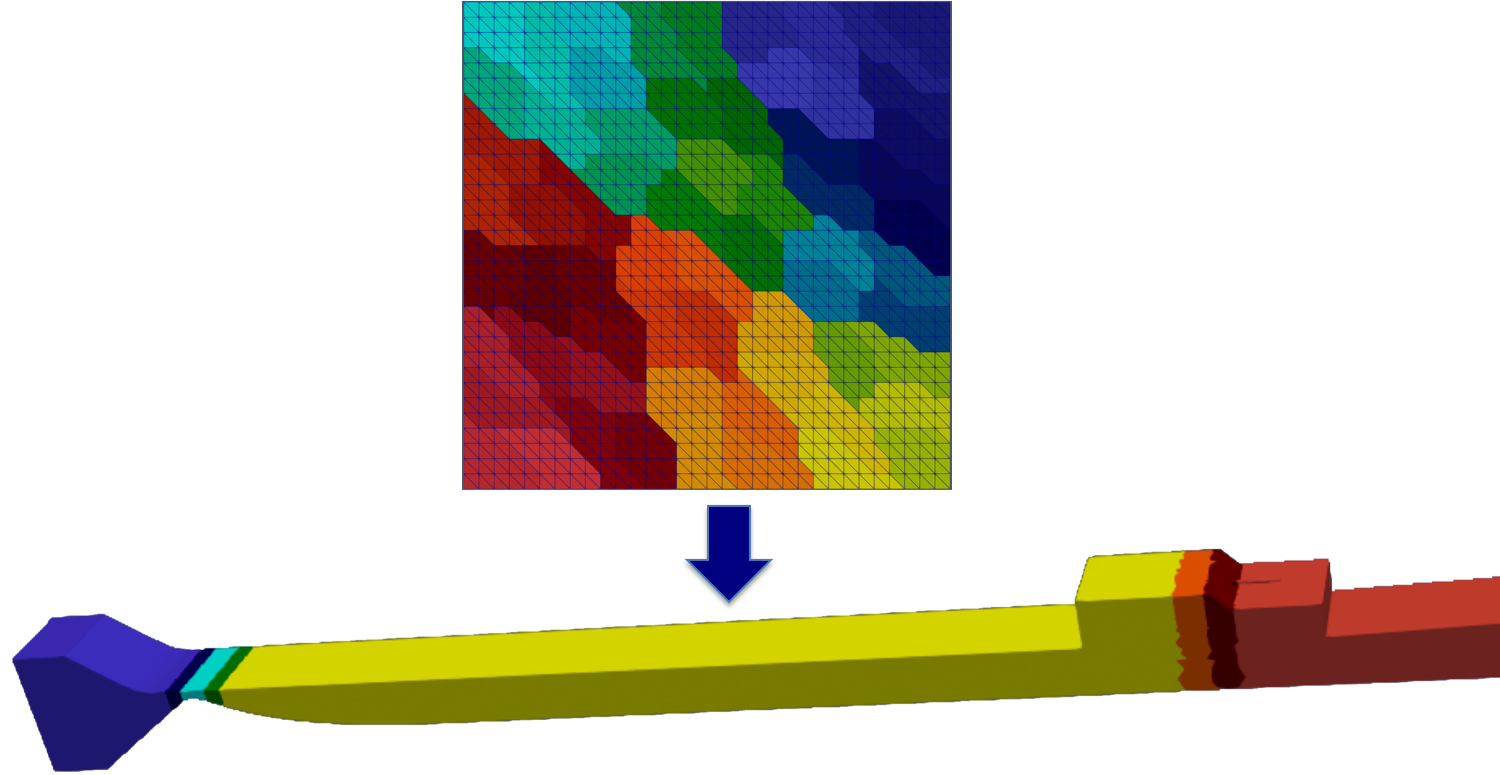
\includegraphics[width=.8\textwidth]{Figures/mtc/MetisTo1D.png} \\
%      \vspace{10pt}
%      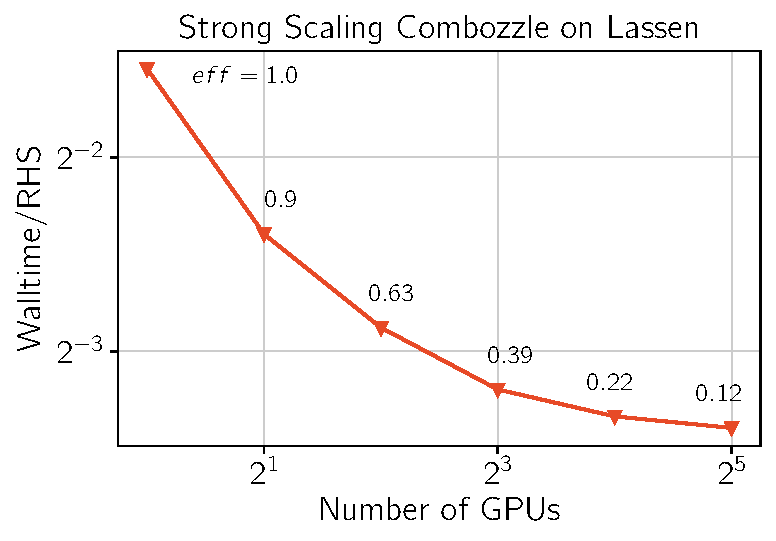
\includegraphics[width=.8\textwidth]{Figures/mtc/combozzle_strong_scaling2.pdf}
%    \end{figure}		
%  \end{minipage}
%\end{frame}

%\begin{frame}\frametitle{DAG Splat Effect}
%\begin{minipage}[t][0.4\textheight][t]{\textwidth}
%\begin{center}
%New: prediction-enabling performance
%\end{center}
%\begin{multicols}{2}
%\begin{itemize}
%\item DAG Splat: DAG for each boundary
%\item Limits weak scaling - DAG for each neighbor
%\columnbreak
%\item Mitigation: Metis $\to$ 1D decomp
%\item Real fix: Function calls in the DAG (aka function outlining)
%\end{itemize}
%\end{multicols}
%\end{minipage}\vfill
%\vspace{-20pt}
%\begin{minipage}[t][0.4\textheight][t]{\textwidth}
%\centering
%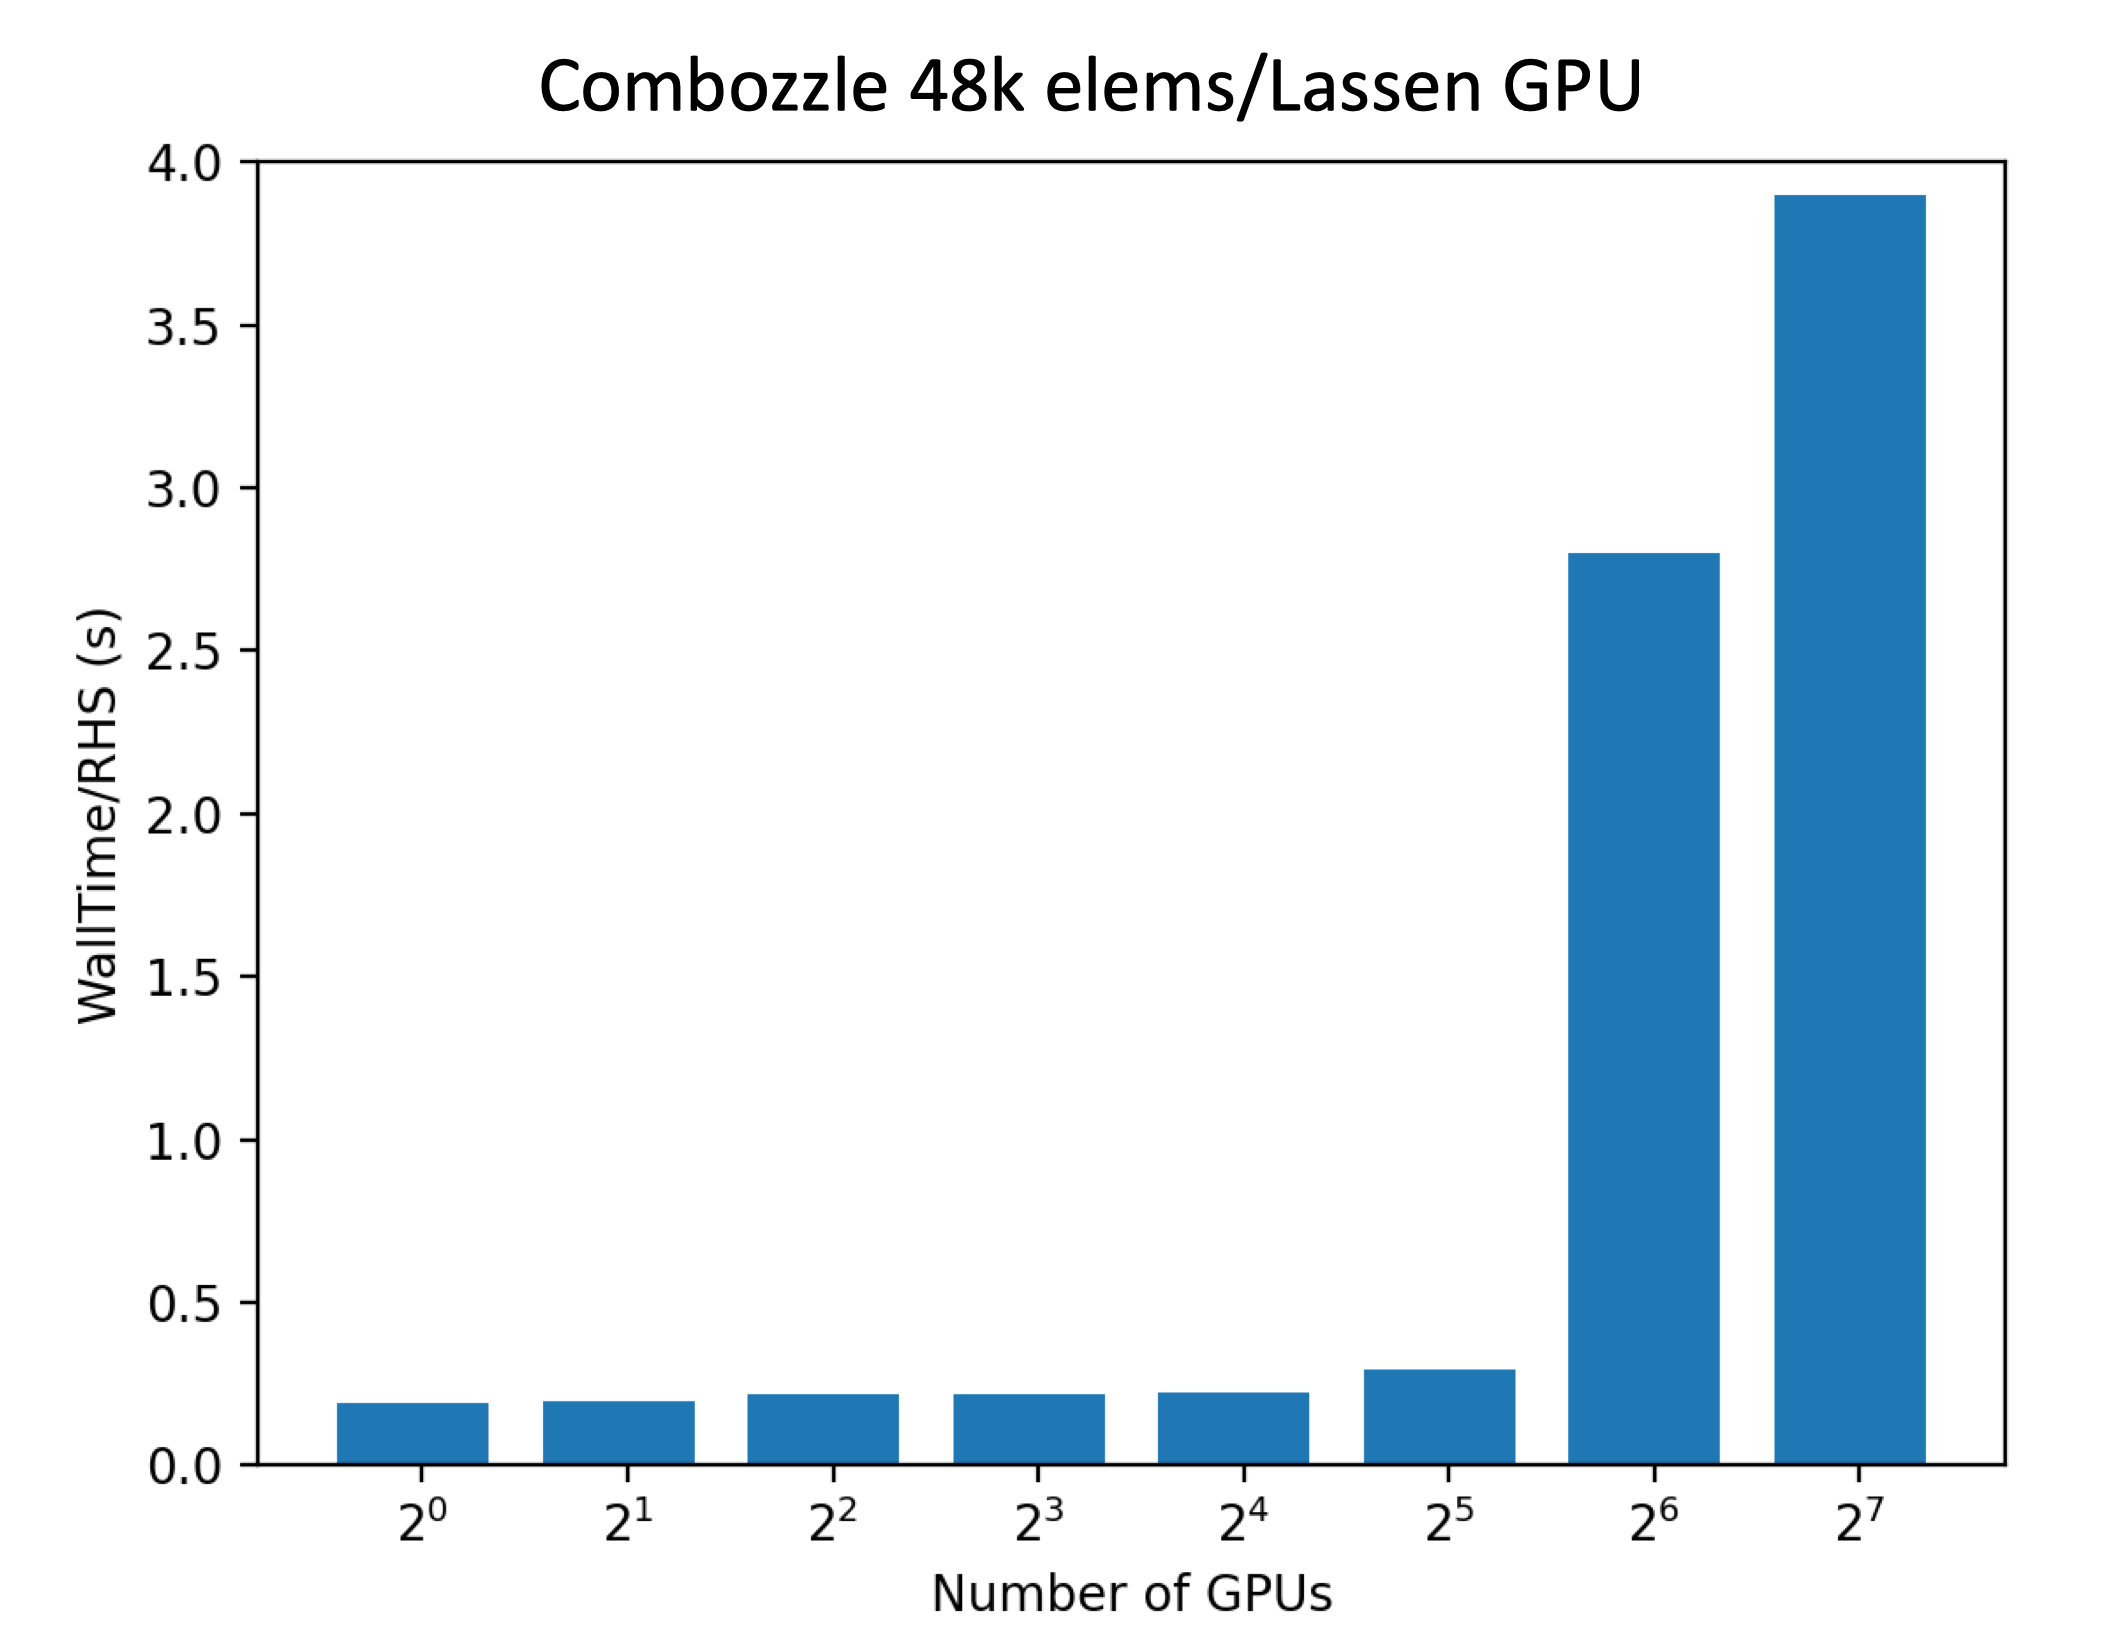
\includegraphics[width=.4\textwidth]{Figures/mtc/combozzle_weak_bad_partitioning.png}\hspace{30pt}
%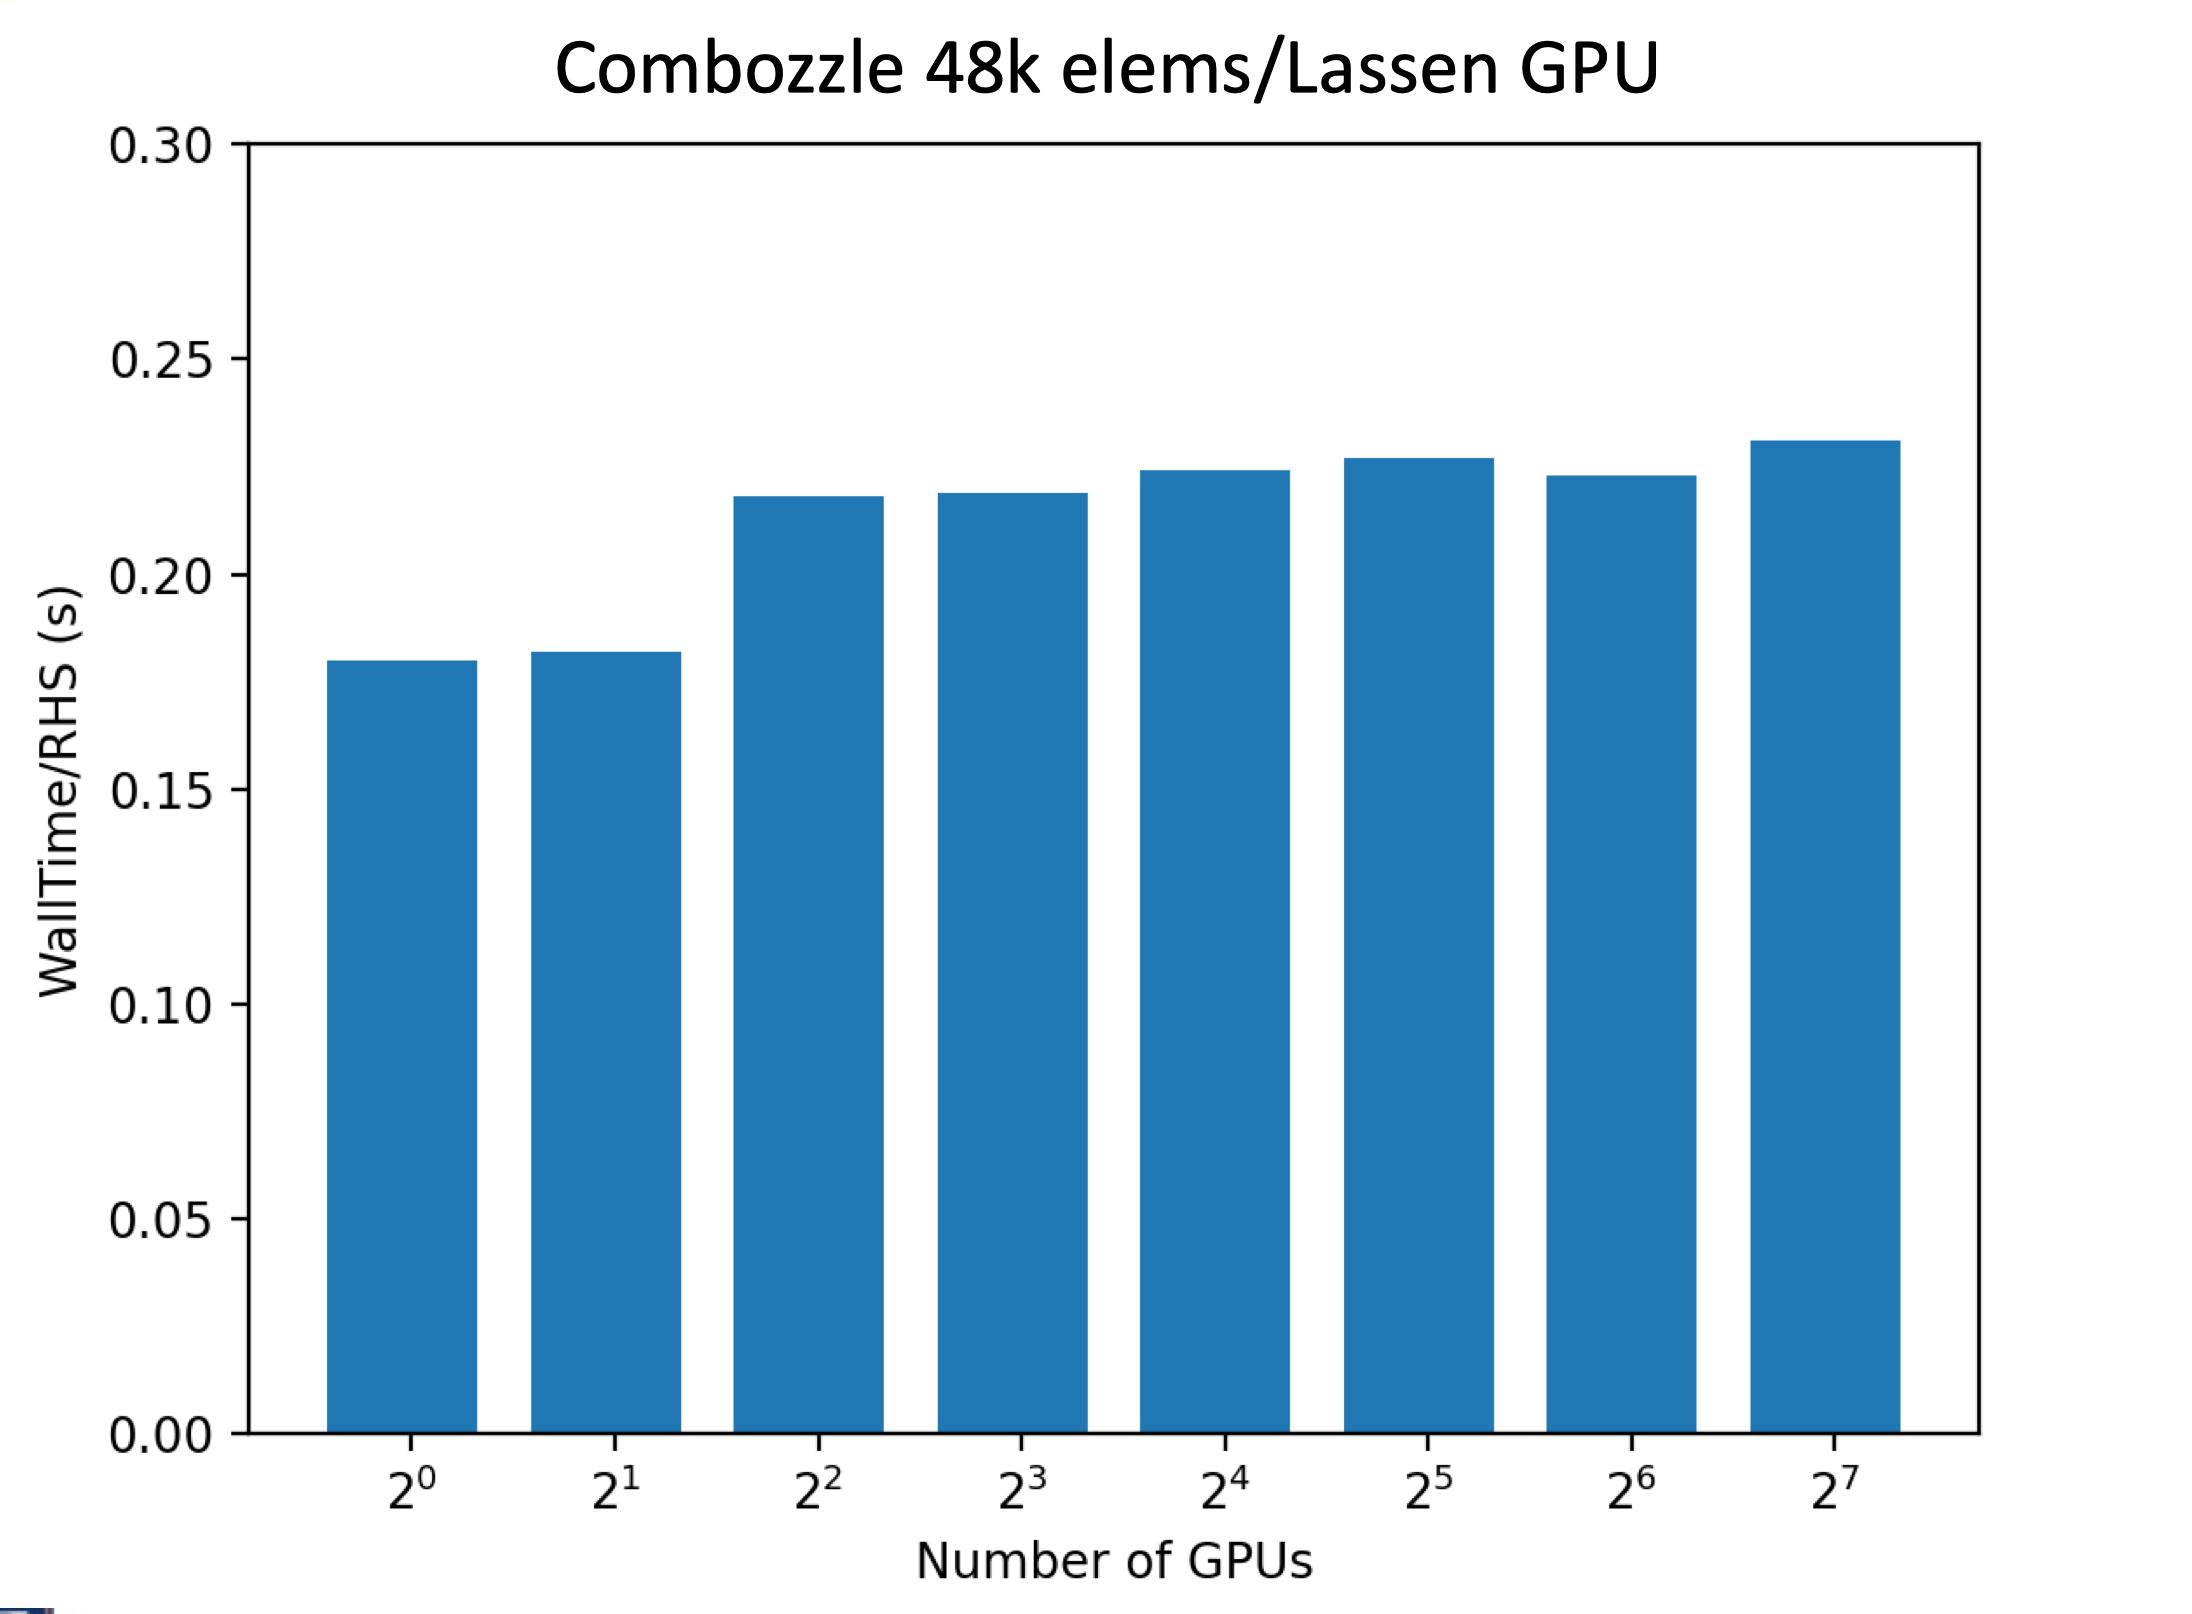
\includegraphics[width=.4\textwidth]{Figures/mtc/combozzle_weak_sliced_partitioning.png}
%\end{minipage}
%\end{frame}

%\begin{frame}\frametitle{DAG Splat Mitigation}
%\begin{minipage}[t][0.4\textheight][t]{\textwidth}
%\begin{center}
%New: prediction-enabling performance
%\end{center}
%\begin{multicols}{2}
%\begin{itemize}
%\item DAG Splat: DAG for each boundary
%\item Limits weak scaling - DAG for each neighbor
%\columnbreak
%\item Mitigation: Metis $\to$ 1D decomp
%\item Real fix: Function calls in the DAG (a.k.a. outlining)   %\prj\tiny{Kaushik Kulkarni}
%\end{itemize}
%\end{multicols}
%\end{minipage}\vfill
%%\vspace{-100pt}
%\begin{minipage}[t][0.4\textheight][t]{\textwidth}
%\centering
%%\includegraphics[width=.9\textwidth]{Figures/mtc/1dpart_bal.png}\\
%\includegraphics[width=.9\textwidth]{Figures/mtc/1dpartshiny.png}\\
%%\vspace{-50pt}
%\begin{center}
%Y2 Domain Decomposition
%\end{center}
%\end{minipage}
%\end{frame}

%\begin{frame}\frametitle{Scaling with 1D Partitioning}
%\begin{minipage}[t][0.4\textheight][t]{\textwidth}
%\begin{center}
%New: prediction-enabling performance
%\end{center}
%\begin{multicols}{2}
%\begin{itemize}
%\item DAG Splat: DAG for each boundary
%\item Limits weak scaling - DAG for each neighbor
%\columnbreak
%\item Mitigation: Metis vs. 1D decomp
%\item Real fix: Function calls in the DAG (a.k.a. outlining)  \prj\tiny{M.~Smith}% \prj\tiny{Kaushik Kulkarni}
%\end{itemize}
%\end{multicols}
%\end{minipage}\vfill
%\vspace{-20pt}
%\begin{minipage}[t][0.4\textheight][t]{\textwidth}
%\centering
%%\includegraphics[width=.48\textwidth]{Figures/mtc/y2ks3d_weak.png}
%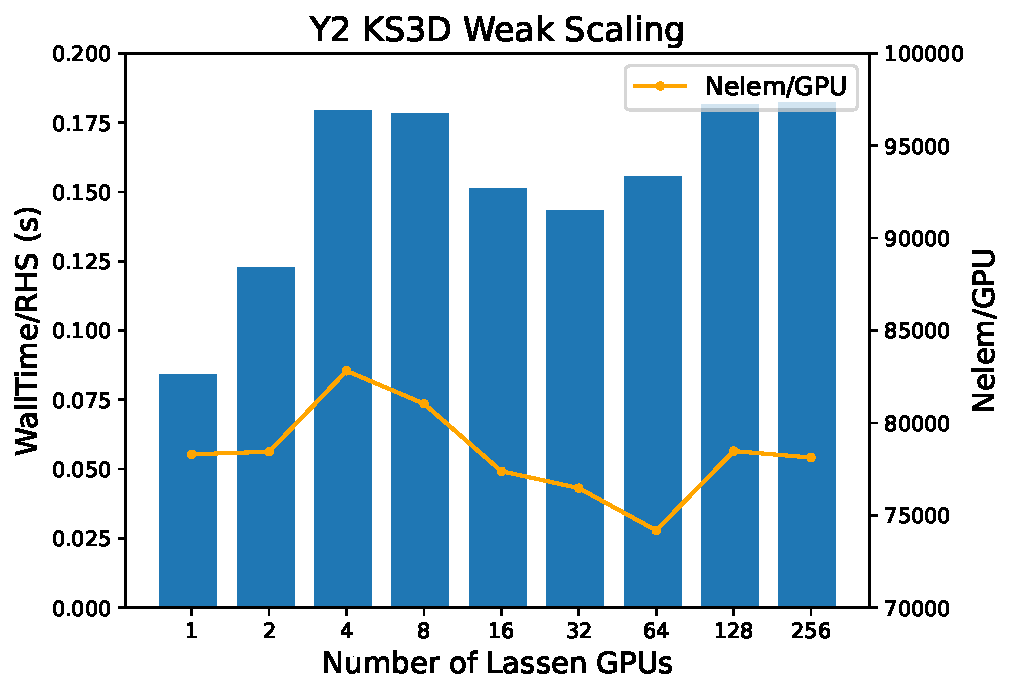
\includegraphics[width=.48\textwidth]{Figures/mtc/y2-prediction_weak_scaling.pdf}
%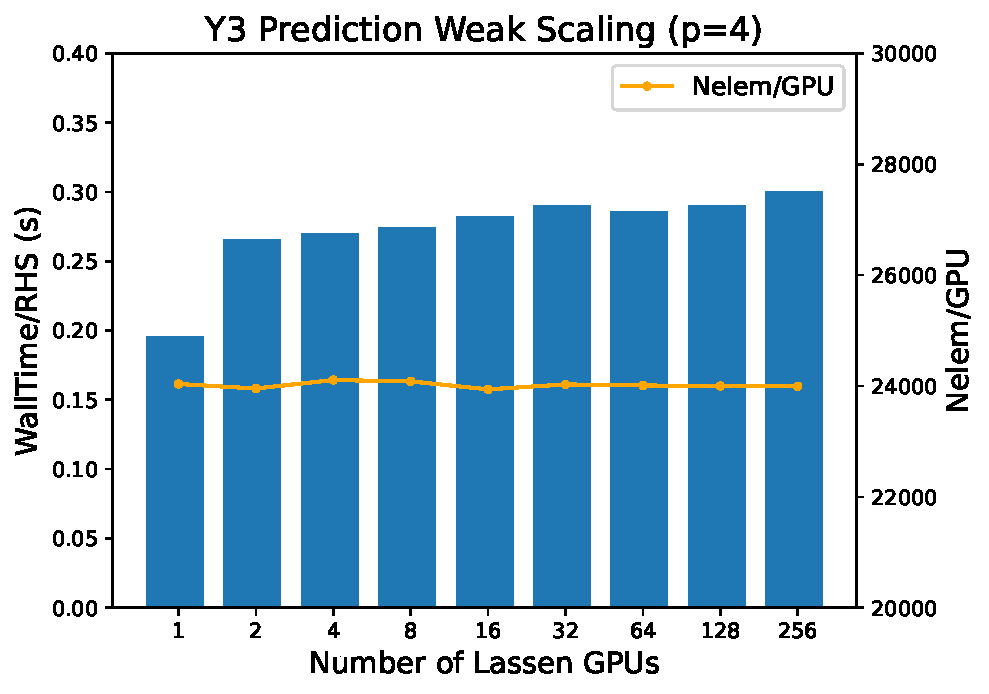
\includegraphics[width=.48\textwidth]{Figures/mtc/y3-prediction_weak_scaling.pdf}
%\end{minipage}
%\end{frame}


%\newcommand{\softwaredeps}{
%  \input{./Figures/software.tikz}
%}

%\begin{frame}\frametitle{Flowchart Example}
%
%% Define styles for the flowchart
%\tikzstyle{startstop} = [rectangle, rounded corners, minimum width=3cm, minimum height=1cm,text centered, draw%=black, fill=red!30]
%\tikzstyle{io} = [trapezium, trapezium left angle=70, trapezium right angle=110, minimum width=3cm, minimum he%ight=1cm, text centered, draw=black, fill=blue!30]
%\tikzstyle{process} = [rectangle, minimum width=3cm, minimum height=1cm, text centered, draw=black, fill=orang%e!30]
%\tikzstyle{decision} = [diamond, minimum width=3cm, minimum height=1cm, text centered, draw=black, fill=green!%30]
%\tikzstyle{arrow} = [thick,->,>=stealth]
%% Draw the flowchart
%\begin{tikzpicture}[node distance=2cm]
%
%\node (start) [startstop] {Start};
%\node (in1) [io, below of=start] {Input};
%\node (pro1) [process, below of=in1] {Process 1};
%\node (dec1) [decision, below of=pro1] {Decision 1};
%\node (pro2a) [process, left of=dec1, xshift=-2cm] {Process 2a};
%\node (pro2b) [process, right of=dec1, xshift=2cm] {Process 2b};
%\node (out1) [io, below of=dec1] {Output};
%\node (stop) [startstop, below of=out1] {Stop};
%
%\draw [arrow] (start) -- (in1);
%\draw [arrow] (in1) -- (pro1);
%\draw [arrow] (pro1) -- (dec1);
%\draw [arrow] (dec1) -- node[anchor=east] {yes} (pro2a);
%\draw [arrow] (dec1) -- node[anchor=west] {no} (pro2b);
%\draw [arrow] (pro2a) |- (out1);
%\draw [arrow] (pro2b) |- (out1);
%\draw [arrow] (out1) -- (stop);
%
%\end{tikzpicture}
%\end{frame}
%\begin{frame}\frametitle{Flowchart 1}
%\begin{tikzpicture}[
%    % Define arrow style
%    arr/.style={-Stealth, thick},
%    % Define box styles
%    source/.style={draw, rounded corners, fill=blue!20, align=center, minimum height=2em},
%    process/.style={draw, rounded corners, fill=orange!30, align=center, minimum height=2em},
%    file/.style={draw, tape, tape bend top=none, fill=blue!20, align=center, minimum height=2em},
%    database/.style={draw, cylinder, shape border rotate=90, aspect=0.25, fill=blue!20, align=center, minimum %height=2em}
%]

%% Place nodes
%\node[source] (sms) {Serial Mesh\\Source\\(gmsh, meshmode)};
%\node[file, below=0.5cm of sms] (nrestart) {N restart\\pkl files};
%\node[process, right=1cm of nrestart] (meshdist) {meshdist};
%\node[process, right=1cm of meshdist] (mirgecom) {MIRGE-Com\\(M-ranks)};
%\node[file, below=0.5cm of mirgecom] (mrestart) {M restart\\pkl files};
%\node[process, left=1cm of mrestart] (redist) {redist};
%\node[file, left=1cm of redist] (nviz) {N viz vtk files};
%\node[database, below=0.5cm of nrestart] (vizproc) {Visualization\\Processing};
%
% Connect nodes with arrows
%\draw[arr] (sms) -- (nrestart);
%\draw[arr] (nrestart) -- (meshdist);
%\draw[arr] (meshdist) -- (mirgecom);
%\draw[arr] (mirgecom) -- (mrestart);
%\draw[arr] (mrestart) -- (redist);
%\draw[arr] (redist) -- (nviz);
%\draw[arr] (nviz) -- (vizproc);
%\draw[arr] (nrestart.south) -- ++(0,-0.5) -| (vizproc);
%\draw[arr] (redist.south) -- ++(0,-0.5) -| (meshdist);
%
%% Add more nodes and connections as necessary to match the provided flowchart
%
%\end{tikzpicture}
%
%\end{frame}
